\documentclass[conference]{IEEEtran}
\IEEEoverridecommandlockouts
% The preceding line is only needed to identify funding in the first footnote. If that is unneeded, please comment it out.
%\usepackage{latex8}
\usepackage{times}
\usepackage{amssymb}
\usepackage{amsmath}
\usepackage{graphicx}
\usepackage{epstopdf}
\usepackage{subfigure}
\usepackage[compress]{cite}
\usepackage{algorithm}
\usepackage{algorithmic}
\usepackage{titlesec}
\usepackage{multirow}
\usepackage{tabularx}
\usepackage{booktabs}
\usepackage{threeparttable}
\usepackage[normalem]{ulem}
\usepackage{url}
\usepackage{CJK}
%\usepackage{amsthm}
\pagestyle{plain}
\usepackage{geometry}
\usepackage{tikz}
\geometry{left=1.5cm,right=1.5cm,top=1.5cm,bottom=1.55cm}


%%\geometry{left=1.40cm,right=1.40cm,top=1.33cm,bottom=2.1cm}
%%\linespread{0.986}
%\setlength{\abovedisplayskip}{1 mm}
%\setlength{\belowdisplayskip}{0.5 mm}
%%\setlength{\abovecaptionskip}{0.0pt}
%%\setlength{\belowcaptionskip}{0.0pt}
%%\titlespacing{\section}{0pt}{4pt}{0 pt}
%%\titlespacing{\subsection}{0pt}{2pt}{0pt}
%%\titlespacing{\subsubsection}{0pt}{2pt}{0pt}
\usepackage[colorlinks,linkcolor=red,anchorcolor=blue]{hyperref}

\newcommand{\songti}{\CJKfamily{song}}

\newcommand{\rev}[1]{\uwave{#1}}
%\newcommand{\rev}[1]{#1}
%\renewcommand{\algorithmicrequire}{\textbf{Input:}}
%\renewcommand{\algorithmicensure}{\textbf{Output:}}

\newcommand{\del}[1]{\sout{#1}}  %revise the text
%\newcommand{\del}[1]{}

\newcommand{\note}[1]{{\sffamily\itshape\bfseries\uline{#1}}}

\newcommand{\addNewNodeCost}{100}
\newcommand{\transformExistedNodeCost}{100000}
\newcommand{\addNodeComputaionCost}{3}
\newcommand{\addEdgeBandwithCost}{1}
\newcommand{\RelativeCostbetweenComputingBandwidth}{3}
\newcommand{\SubstrateNewtorkRunTimeInterval}{300}
\newcommand{\unitTimeInterval}{1}
\newcommand{\requestAppearProbability}{0.5}
\newcommand{\RequestPerTimeAppearNum}{1}
\newcommand{\VNRequestsDuration}{1}
\newcommand{\PossionMean}{5}
\newcommand{\VNRequestsContinueTimeMinimum}{1}
\newcommand{\VNRequestsContinueTimeMaximum}{100}
\newcommand{\VNRequestsContinueTimeAverage}{50}
\newcommand{\VNRequestsContinueTimeExponentialMean}{15}
\newcommand{\SubStrateNodeSize}{30}
\newcommand{\SubStrateNodeComputationMinimum}{20}
\newcommand{\SubStrateNodeComputationMaximum}{50}
\newcommand{\SubStrateNodenodeProbability}{0.75}
\newcommand{\SubStrateEdgeBandwithMinimum}{50}
\newcommand{\SubStrateEdgeBandwithMaximum}{100}
\newcommand{\VirtualNodeSizeMinimum}{3}
\newcommand{\VirtualNodeSizeMaximum}{10}
\newcommand{\VirtualNodeComputationMinimum}{1}
\newcommand{\VirtualNodeComputationMaximum}{5}
\newcommand{\VirtualNodenodeProbability}{0.5}
\newcommand{\VirtualEdgeBandwithMinimum}{5}
\newcommand{\VirtualEdgeBandwithMaximum}{10}
\newcommand{\SubStrateFacilityNodeFailDuration}{12}
\newcommand{\ExperimentTimes}{36}


\newcommand{\MyProblemAbrreviation}{EVSNR }
\newcommand{\CSLIs}{Conflicting SRLG(Shared Risk Link Group) Link Inclusion Set of graph $G^*$ }
\newcommand{\CEs}{$\mathbb{CSLE}^*$ }
\newcommand{\CIs}{$\mathbb{CSLI}^*$ }



\newtheorem{theorem}{Theorem}
\newtheorem{lemma}{Lemma}
\newtheorem{definition}{Definition}



\begin{document}
%\begin{CJK*}{GBK}{song}

\title{Survivable embedded Virtual Network Design to Survive a Facility Node Failure\\
%{\footnotesize \textsuperscript{*}Note: Sub-titles are not captured in Xplore and should not be used}
\thanks{Identify applicable funding agency here. If none, delete this.}
}

\author{\IEEEauthorblockN{Kun Xie$^1$}
\IEEEauthorblockA{\textit{College of Computer Science and Electronic Engineering} \\
\textit{Hunan University}\\
Chang Sha, China \\
kun.xie@stonybrook.edu}
\and
\IEEEauthorblockN{Heng Tao}
\IEEEauthorblockA{\textit{College of Computer Science and Electronic Engineering} \\
\textit{Hunan University}\\
Chang Sha, China\\
franztaoheng@gmail.com}
\and
\IEEEauthorblockN{3\textsuperscript{rd} Given Name Surname}
\IEEEauthorblockA{\textit{dept. name of organization (of Aff.)} \\
\textit{name of organization (of Aff.)}\\
City, Country \\
email address}
\and
\IEEEauthorblockN{4\textsuperscript{th} Given Name Surname}
\IEEEauthorblockA{\textit{dept. name of organization (of Aff.)} \\
\textit{name of organization (of Aff.)}\\
City, Country \\
email address}
\and
\IEEEauthorblockN{5\textsuperscript{th} Given Name Surname}
\IEEEauthorblockA{\textit{dept. name of organization (of Aff.)} \\
\textit{name of organization (of Aff.)}\\
City, Country \\
email address}
}

\maketitle
\vspace{-3em}
%\vspace{-0.6in}
\begin{abstract}
Ensuring transmission survivability is a crucial problem for high-speed networks. Path protection is a fast and capacity-efficient approach for increasing the availability of end-to-end connections. The emerging SDN infrastructure makes it feasible to provide diversity routing in a practical network. For more robust path protection, it is desirable to provide an alternative path that does not share any risk resource with the active path. We consider finding the SRLG-Disjoint paths, where a Shared Risk Link Group (SRLG) is a group of network links that share a common physical resource whose failure will cause the failure of all links of the group. Since the traffic is carried on the active path most of time, it is useful that the weight of the shorter path of the disjoint path pair is minimized, and we call it  Min-Min SRLG-Disjoint routing problem. The key issue faced by SRLG-Disjoint routing is the trap problem, where the SRLG-disjoint backup path (BP) can not be found after an active path (AP) is decided. Based on the min-cut of the graph, we  design an  efficient algorithm that can  take advantage of existing search results to quickly look for the SRLG-Disjoint path pair. Our performance studies demonstrate that our algorithm can outperform other approaches with a higher routing performance while also at a much faster speed.
\end{abstract}


\begin{IEEEkeywords}
NFV, VNE, Survivability
\end{IEEEkeywords}

\section{Introduction}
\label{sec:Introduction}
why network virtualization is significant.

network virtualization has gained significant attention in recent years as an effective means to share substrate network (SN) infrastructure among several virtual network (VN) service providers so as to improve the utilization of the substrate resources \cite{armbrust2009above,yu2008rethinking}. In the network virtualization environment, provisioning a VN is a promising way to support distributed applications and services which require the coordination of multiple geographically distributed facilities (e.g. storage arrays or computer clusters). With the maturity of the optical network technology and their high-bandwidth and low-latency characteristics, we will be able to deploy a federated computing and networking system (FCNS) \cite{zhang2013effective,papagianni2013optimal}, which interconnects a large number of facility nodes with optical network managed or controlled integratedly, to enable such large scale distributed applications.

Network virtualization is a promising technology to reduce the operating costs and management complexity of networks, and it is receiving an increasing amount of research interest\cite{chowdhury2009network}. Survivability is bound to become a more prominent issue as infrastructure providers move toward virtualizing their networks over cheaper commodity hardware\cite{bhatia2008trellis}. we are concerned with critical virtual nodes and embedding them as an entire infrastructure with survivability guarantees. Fault tolerance is provided in data centers \cite{guo2009bcube} through excessive redundant nodes and links organized in a special way. These works provide Survivability but do not customize survivability guarantees to embedded VInfs. However, such slice is not used as a back-up, but as a monitoring tool, and as a way to debug
the network in the case of failure.\cite{wang2008virtual} considered the use
of virtualized router as a management primitive that can be used to migrate routers for maximal reliability.

what is VN

In network virtualization, the primary entity is the Virtual Network (VN). A VN is a combination of active and passive network elements (network nodes and network links) on top of a Substrate Network (SN). Virtual nodes are interconnected through virtual links, forming a virtual topology. By virtualizing both node and link resources of a SN, multiple virtual network topologies with widely varying characteristics can be created and co-hosted on the same physical hardware.
Each VN request consists of a collection of virtual (task) nodes connected together by a set of virtual links to form a virtual topology; it also has certain resource requirement, such as computing resources for the nodes and bandwidth resources for the links. Such VN request could be represented by a task graph. To establish the VN, one needs to embed task nodes onto facility nodes, and virtual edges onto one or more substrate paths\cite{yu2008rethinking} , as well as allocating sufficient substrate resources which should not violate the computing/ bandwidth capacity limits of facility node/substrate link.



why node failure happern

With infrastructure rapidly becoming virtualized, shared and dynamically changing, it is essential to have strong reliability support from the physical infrastructure, since a single physical server or link failure affects several shared virtualized entities. Providing survivability is often linked with over-provisioning both computational and network capacities, and employing load balancing for additional robustness. Such highly survivable systems are good for applications where large discontinuity may be tolerable, e.g. restart of network flows while rerouting over link or node failures, or partial job restarts at node failures. A higher level of fault tolerance is required at applications where some failures have a substantial impact on the current state of the system. For instance, virtual networks with servers which perform admission control, scheduling, load balancing, bandwidth broking, AAA or other NOC operations that maintain snapshots of the network state, cannot tolerate total failures. In master slave/ worker architectures, e.g. MapReduce, failures at the master nodes waste resources at the slaves/workers, we do not talk about the capacity requirement and geographical location requirement of virtual node, and the bandwidth capacity requirement of virtual link in this paper.

what situation happen

In the multi-tenant network virtualization environment, one challenging problem raised is how to efficiently embed VN requests with various constraints. This is of utmost importance for increasing the utilization of SN resources and infrastructure providers’ revenue \cite{koponen2014network}. Survivable virtual network embedding deals with failures in the substrate and virtual network. The challenges to be considered are link and node failures, which have to be backed up before the failure or recovered after failure. Failures can occur at different layers in the network. For example at the physical layer, a fiber cut
may cause a physical dis-connectivity. In\cite{markopoulou2004characterization}, it is shown that 20 \% of all failures in an IP backbone are resulting from
maintenance activities. About 53 \% of the unplanned link failures are due to router-related \cite{markopoulou2004characterization}. In a network, single
and also multiple failures can occur. The single failure case happens more often than multiple simultaneous failures. The study \cite{markopoulou2004characterization} states that about 70 \% of the unplanned link failures are single link failures. A study \cite{gill2011understanding} about network-related failures in data centers found out that link failures happen about ten times more than node failures per day. Usually node failures are due to maintenance \cite{gill2011understanding}.


why survivable eVN is paramount

However, with network virtualization gaining momentum, the survivability challenges in VNE should also be well investigated. In a large networked computing system, hardware and software failures of facility nodes and communication resources (e.g., links and switching nodes) are norm instead of exception, such as power outages caused by virus attack, disk failures, misconfiguration or fiber cut \cite{xu2012survivable,rahman2010survivable,rahman2013svne,guo2011shared,chen2010resilient}. Such failures will force the virtual node (links) assigned to it to be migrated/re-embeded to another facility node at a geographically different location (link disjoint substrate path). This means that, in order to survive from the disruptions due to such failures, one must reserve redundant facility nodes and bandwidth on fiber links such that after any failure when virtual network request had been embedded in substrate network, there are adequate remaining computing and networking resources to migrate/remap the eVN request. In most case, failure occur when VN had been embedded into SN. Accordingly, the problem of minimizing the resources, including computing and communication resources, reserved for VN request to tolerate substrate failures, (hereafter called Survivable eVN problem, SeVN) is both critical and challenging. Actually, SeVN problem is quite different with the protection approach
in IP over WDM network by investigating facility node failure caused virtual node failure problem and employing node migration induced VN remapping as an unique recovery strategy.


why happen Survivable embeded Virtual Network Request

The software-defined NFV architecture further offers agile traffic steering and joint optimization of network functions and resources.
%When a survivable request of virtual network is coming, survivable virtual network requests are associated with node's service functions.
In any real virtual networks, any nodes of virtual network  are deployed with a service function and the corresponding physical node could run some various service functions. After virtual network VN is embedded into substrate network, a running node of physical network could fail multiple virtual network so that we should obtain survivable eVN to be embedded into substrate network so that recovery from the failure even though one or multiple nodes of virtual network failed because these virtual node corresponding substrate node fail. The augmented nodes of survivable embedded virtual network are embedded into substrate network ultimately, the augmented nodes have specific service functions similarly as shown in Fig.\ref{fig:VNmapSN}.

\begin{figure*}
  \centering
  % Requires \usepackage{graphicx}
  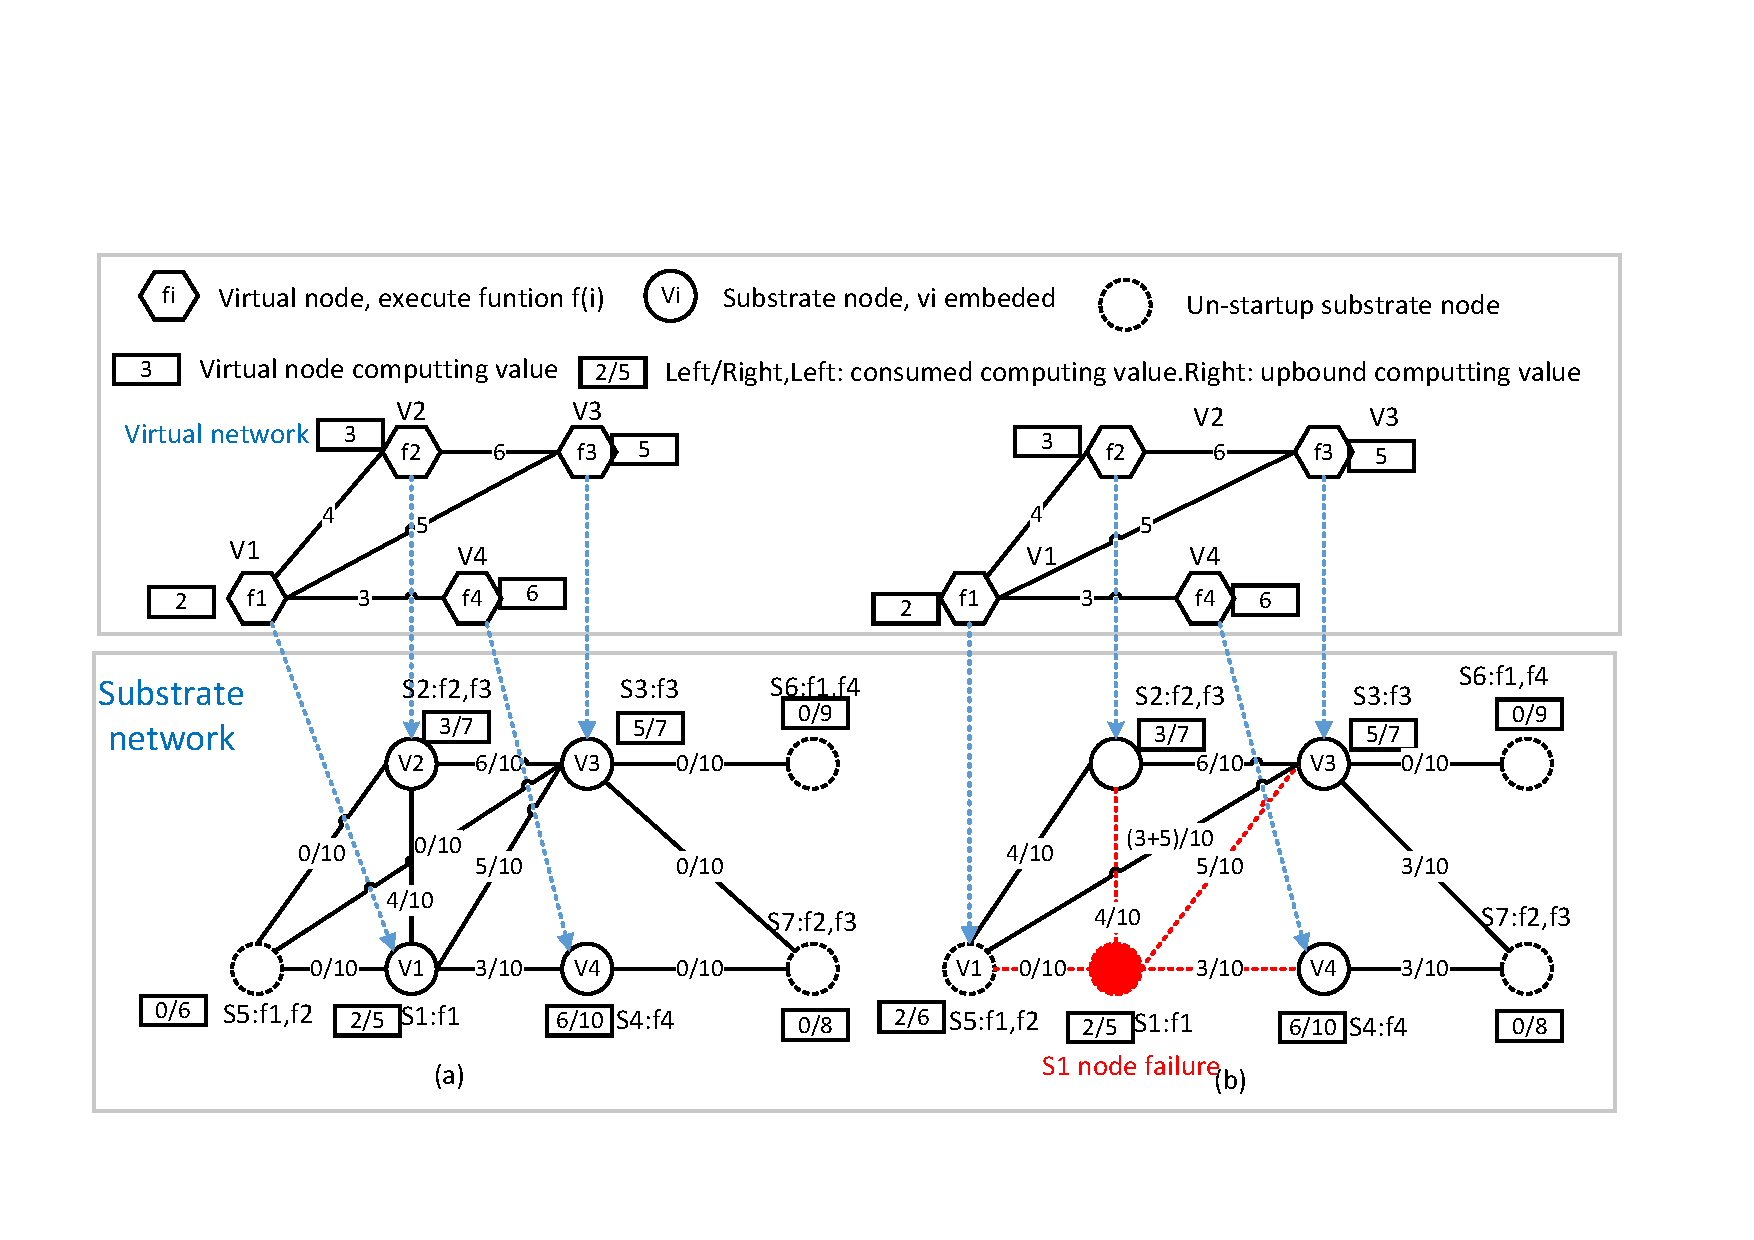
\includegraphics[width=5in]{Fig/VNmapSN}\\
  \caption{function virtual network (VN) embedding and one node failure}\label{fig:VNmapSN}
\end{figure*}

proactive or reactive type

There are two main survivability methods: protection and restoration \cite{ramamurthy2003survivable}. Failure protection is done in a proactive way to reserve the backup resources before any failure happens. Reactive mechanisms, which are called restoration mechanisms, react after the failure occurs and start the backup restoring mechanism. However, some data loss is possible in the reactive case. There exist two kinds of backups for the protection scheme: dedicated backup or shared backup. In shared backup, the resources for the backup may be shared with other backups. In the dedicated case the backup resources are not shared for other backups.


To survive a substrate link failure, pre-computed alternative paths inVN are used in general and the bandwidths are allocated before or after a failure. For instance, the reactive detour solution is employed after a substrate link failure in \cite{rahman2010survivable}, while authors in \cite{rahman2013svne,guo2011shared} propose a proactive backup approach (considering the backup resources sharing) to avoid service disruption in reactive restoration approach and improve the substrate resource utilization.


FD  FI

In terms of SeVN capable of recovering/re-embedding the task nodes after a facility node failure, there are two basic approaches: Failure Dependent Protection (FDP \cite{yu2010survivable} and Failure Independent Protection (FIP) \cite{yeow2011designing}, and the differences between them are as follows. In FIP, a host (facility) node is assigned and dedicated to backup all working host (facility) nodes. That is, no matter which working host node fails, the affected task node will be migrated to the only one backup host node. On the other hand, with FDP, each working host node can have a different backup host node under different failure scenarios. In fact, after a failure, even an unaffected task node may be migrated from a working host node to its corresponding backup host node, as a result of re-embedding the entire task graph. In other words, FDP could provide more flexibility in survivable VN designing by allowing task nodes migrating freely after failure, so FIP could be considered as a special case of FDP and FDP is expected to use fewer resources at the cost of more task nodes migrations after a failure.


Guarantying integration of topological structure of virtual network request is more important than node migration cost when facility node failure.


serive type

Through synchronization\cite{bressoud1996hypervisor,cully2008remus} and migration techniques\cite{clark2005live,wang2008virtual} on virtual machines and routers, we suppose that every virtual network have specific service functions, in addition that fault tolerant can be introduced at the virtualization layer\cite{yeow2011designing}. \cite{qu2016delay}

node cost larger than edge cost

As nodes often represent expensive components (servers) and edges represent less expensive interconnections (links) \cite{armbrust2009above,yu2010survivable}, most attention has been devoted to node faults, i.e., the removal of nodes (and their incident edges), rather than edge faults where only edges are removed.

The node failure type we focus in this paper is independent node failures. multiple independent or dependent failure nodes problem could be discussed in the future.


%
%\begin{table}
%\centering
%\begin{tabular}{cc}
%\hline
%Term & Description \\
%$G(V,E,S)$ & $G(V,E,S)$ denotes the Virtual Network, consisting of nodes V, links E and service functions\\
%$B(V,S)$ & $B(V,S)$ denotes the Backup nodes set, consisting of nodes V and service functions S which is corresponding to every nodes \\
%\hline
%\end{tabular}
%\caption{terminology used throughout this paper}\label{tab:term}
%\end{table}

The organization of this paper is as follow. In the next section, we briefly describe the background, notations and define survivability in Sec.\ref{sec:ProblemFormulation}. Finally, we evaluate and validate the ideas through simulation in Sec.\ref{sec:Evaluation}.

%\section{Related work}
Network virtualization is a promising technology to reduce the operating costs and management complexity of networks, and it is receiving an increasing amount of research interest\cite{chowdhury2009network}. Survivability is bound to become a more prominent issue as infrastructure providers move toward virtualizing their networks over cheaper commodity hardware\cite{bhatia2008trellis}. we are concerned with critical virtual nodes and embedding them as an entire infrastructure with Survivability guarantees. Fault tolerance is provided in data centers \cite{guo2009bcube} through excessive redundant nodes and links organized in a special way. These works provide Survivability but do not customize Survivability guarantees to embedded VInfs. However, such slice is not used as a back-up, but as a monitoring tool, and as a way to debug
the network in the case of failure.\cite{wang2008virtual} considered the use
of virtualized router as a management primitive that can be used to migrate routers for maximal reliability.

\subsection{Types and characteristics of failures} Survivable virtual
network embedding deals with failures in the substrate and
virtual network. The challenges to be considered are link and
node failures, which have to be backed up before the failure
or recovered after failure. Failures can occur at different layers
in the network. For example at the physical layer, a fiber cut
may cause a physical dis-connectivity. In\cite{markopoulou2004characterization}, it is shown
that 20 \% of all failures in an IP backbone are resulting from
maintenance activities. About 53 \% of the unplanned link
failures are due to router-related \cite{markopoulou2004characterization}. In a network, single
and also multiple failures can occur. The single failure case
happens more often than multiple simultaneous failures. The
study \cite{markopoulou2004characterization} states that about 70 \% of the unplanned link failures
are single link failures. A study \cite{gill2011understanding} about network-related
failures in data centers found out that link failures happen
about ten times more than node failures per day. Usually node
failures are due to maintenance \cite{gill2011understanding}.

\subsection{Survivable failure methods} There are two main survivability methods: protection and restoration \cite{ramamurthy2003survivable}. Failure protection is done in a proactive way to reserve the backup resources before any failure happens. Reactive mechanisms, which are called restoration mechanisms, react after the failure occurs and start the backup restoring mechanism. However, some data loss is possible in the reactive case. There exist two kinds of backups for the protection scheme: dedicated backup or shared backup. In shared backup, the resources for the backup may be shared with other backups. In the dedicated case the backup resources are not shared for other backups.

Meanwhile some works address node fault tolerance at the virtualization level. Bressoud \cite{bressoud1996hypervisor} was the first few to introduce fault tolerance at the hypervisor. Two virtual slices residing on the same physical node can be made to operate in sync through the hypervisor on the same physical node. Others \cite{wang2008virtual,cully2008remus} have made progress for the virtual slices to be duplicated and migrated over a network. Various duplication techniques and migration protocols were proposed for different types of applications (web servers, game servers, and benchmarking applications) \cite{wang2008virtual,cully2008remus} and Kemari \cite{tamura2008kemari} are two other systems that allows for state synchronization between two virtual nodes for full, dedicated
redundancy. However, these works focus on the practical issues, and do not address the resource allocation issue. VNsnap \cite{kangarlou2009vnsnap} is another method to take static snapshots of an entire virtual infrastructure to some reliable storage, in order to recover from failures. This can be stored as reliably
in a distributed manner as replicas \cite{chang2008bigtable}, or as parities \cite{dimakis2006decentralized,yeow2011highly}. VNsnap does not address synchronization, nor guarantee sufficient resources for recovery from snapshots. Fundamentally, there are methods to construct topologies for redundant nodes that address both nodes and links reliability \cite{ajtai1992fault,dutt1997node}. Based on some input graph, additional links are introduced such that the least number is needed. However, a node failure, in this case, may involve migrations among the remaining nodes to preserve the original topology. This may not be suitable in a scenario where migrations
may disrupt other running parts of the network.

%Our problem involves virtual network embedding [8, 18]
%with added node and link redundancy for reliability. Our
%model employs the use of path-splitting [26], which allows a
%link to be split over multiple routes such that the aggregate
%flow across those routes equal to the demand between the
%two nodes. This gives more resilience to link failures and
%allows for graceful degradation. A related work that does
%not use path-splitting for embedding reliability is [16].

%Zhang et al. [7,8] have considered substrate resource sharing among multiple virtual networks. However, their method only con- siders substrate resource sharing within the same priority class and does not consider sharing among different priority classes while at the same time satisfying the different latency require- ments. Thus, the method cannot be applied to the VNE problem where substrate resource sharing among multiple priority classes is required within each requested virtual network. This paper pro- poses a heuristic VNE method to minimize the required amount of substrate resources due to fair substrate resource sharing among multiple virtual networks, while considering the existence of mul- tiple priority classes that share the substrate resources with one another within each virtual network. Since substrate resource shar- ing among multiple virtual networks is expected to occur on the substrate link bandwidth more frequently, the proposed heuris- tic method prioritizes virtual link assignment rather than virtual node assignment, in contrast to most of the existing heuristic methods.

The organization of this paper is as follow. In the next section, we briefly describe the background, notations and define survivability in Sec.\ref{sec:ProblemFormulation}. Finally, we evaluate and validate the ideas through simulation in..

\section{System model and problem}
\label{sec:Problem description}
In this section, we first introduce  basic concepts on virtual network embedding, then present our survivable virtual network embedding problem.


\subsection{Virtual network embedding}


We represent a \textbf{virtual network} (VN) as an undirected graph $G (V,E)$ where $V$ and  $E$ are the sets of virtual nodes and virtual links, respectively. Each virtual link $e_{ij}$ has the bandwidth demand $d_{ij}$. Each virtual node  $v_i$ has the computation capacity demand   $d_i$. For virtual node $v_i$, the virtual function required to be executed on the virtual node is denoted as $f(i)$. Fig.\ref{fig:VNQSNVNE}(a) shows an example virtual network with virtual node set $V=\{v_1,v_2,v_3,v_4\}$ and virtual edge set $E= \{e_{12},e_{13},e_{14},e_{23}\}$. The virtual functions required to be executed on these virtual nodes are  $f(1)=f_1$, $f(2)=f_2$, $f(3)=f_3$, $f(4)=f_4$, respectively.
%\begin{figure}
%\centering
%\begin{minipage}[t]{0.45\linewidth}
%% Requires \usepackage{graphicx}
%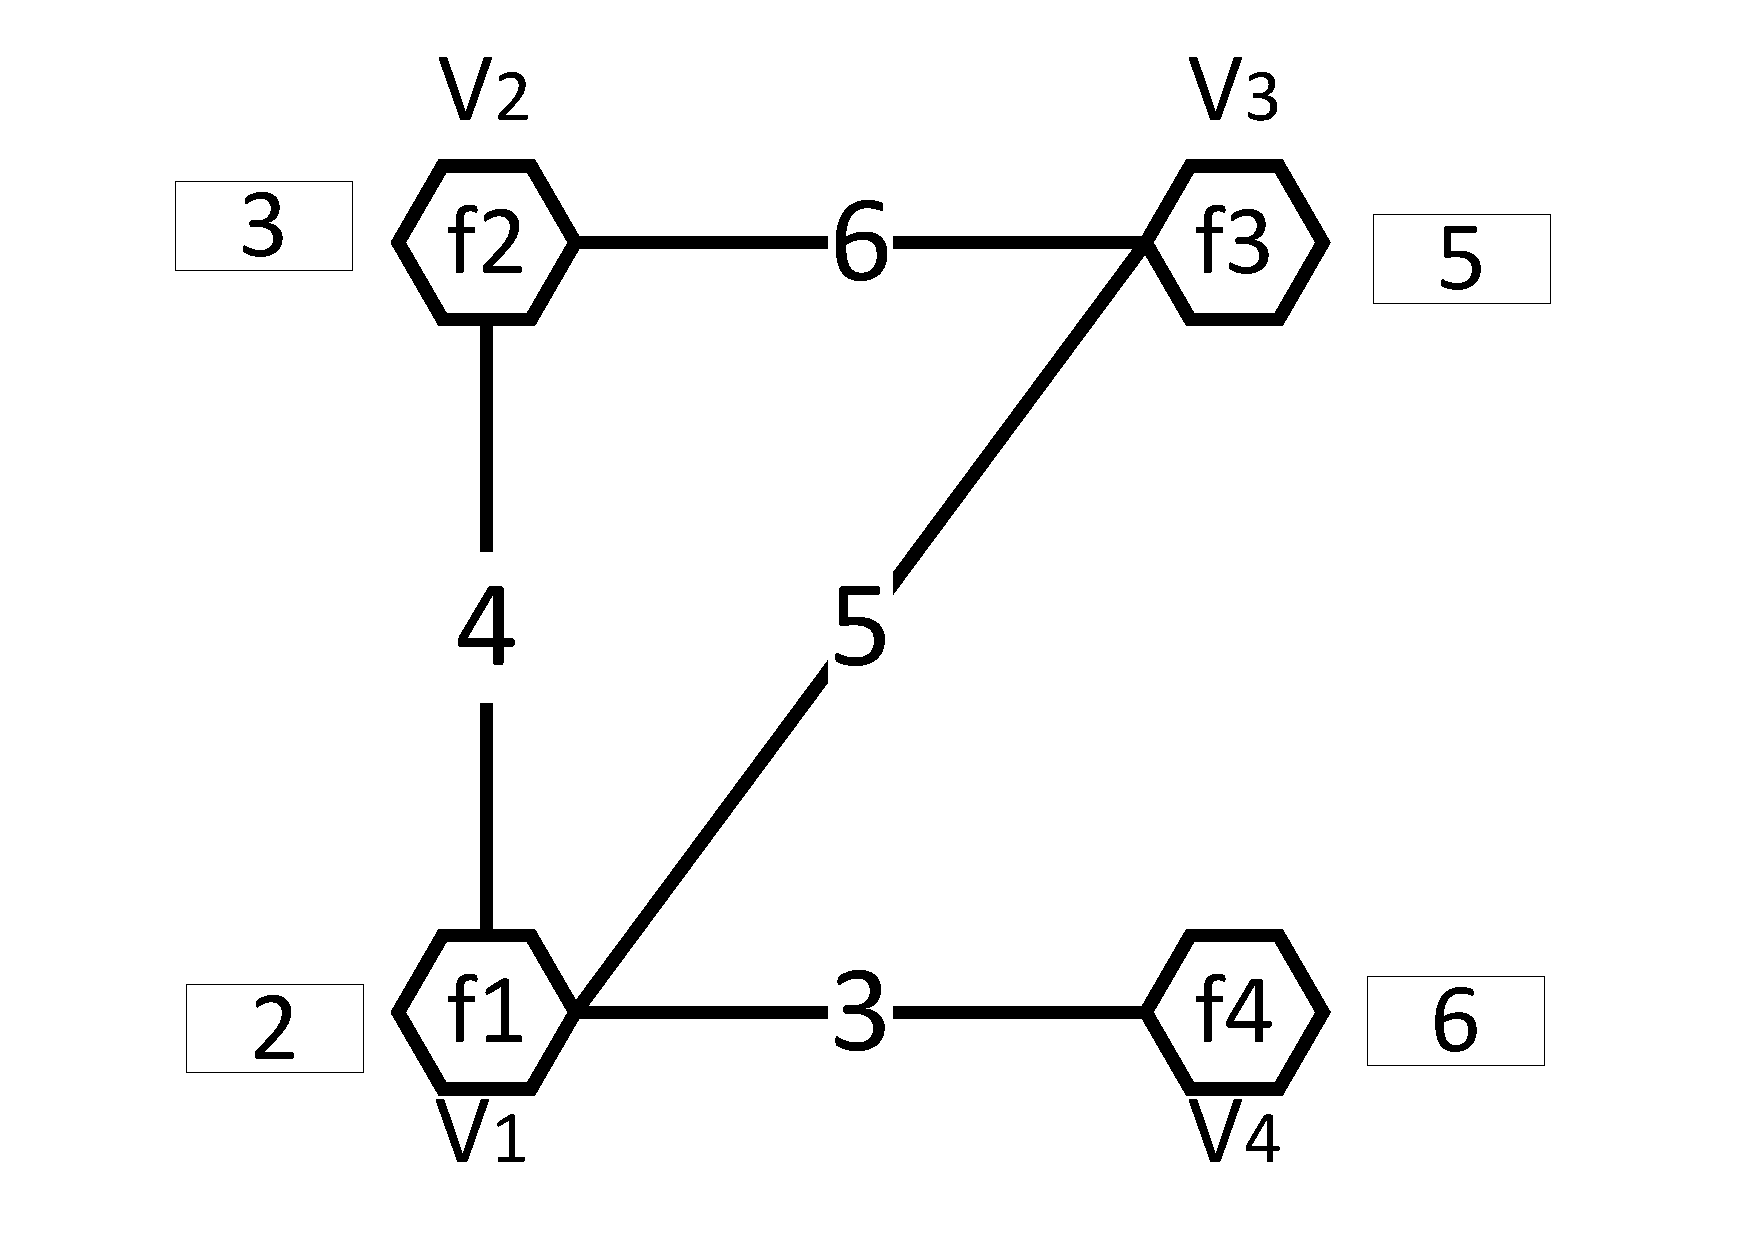
\includegraphics[width=1.3in]{Fig/VNQ}\\
%\caption{Virtual Network Request $G(V,E)$, $V=\{v_1,v_2,v_3,v_4\}$, $E=\{e_{12},e_{23},e_{13},e_{14}\}$,  $f^V=\{f_1,f_2,f_3,f_4\}$, $d_i=\{2,3,5,6\}$, $d_{ij}=\{4,5,3,6\}.$}\label{fig:VNQ}
%\end{minipage}
%\hfill
%\begin{minipage}[t]{0.45\linewidth}
%% Requires \usepackage{graphicx}
%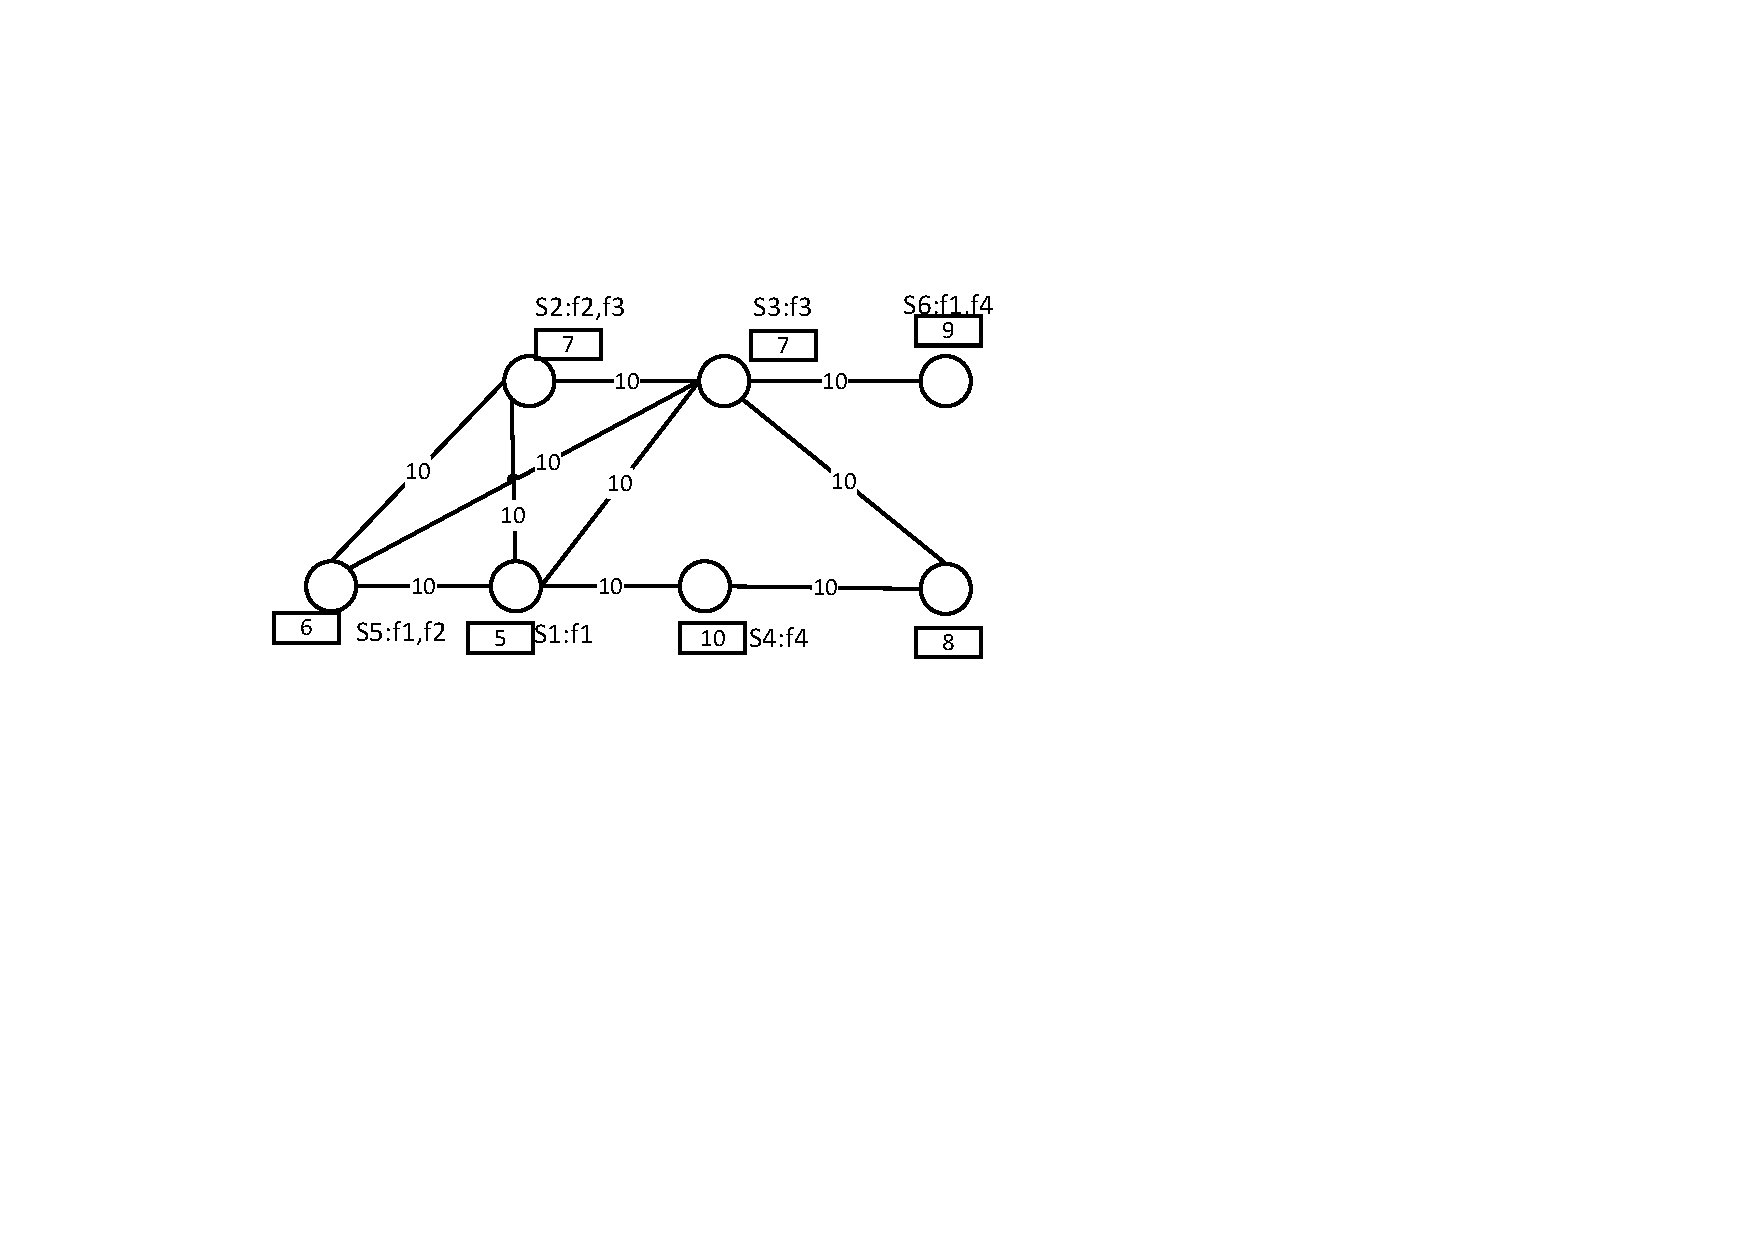
\includegraphics[width=1.8in]{Fig/SN}\\
%\caption{Physical Network $G^S(V^S,E^S), V^S=\{s_1,s_2,s_3,s_4,s_5,s_6,s_7\}, E^S=\{l_{12},l_{13},l_{14},l_{15},l_{23},l_{25},l_{35},l_{36},l_{37},l_{47}\}, F^S=\{\{f_1\},\{f_2,f_3\},\{f_3\},\{f_4\},\{f_1,f_2\},\{f_1,f_4\},\{f_2,f_3\}\}, c_i=\{5,7,7,10,6,9,8\}, %b_{ij}=\{10,10,10,10,10,10,10,10,10,10\}$}\label{fig:SN}
%\end{minipage}
%\end{figure}

\begin{figure*}
\centering
% Requires \usepackage{graphicx}
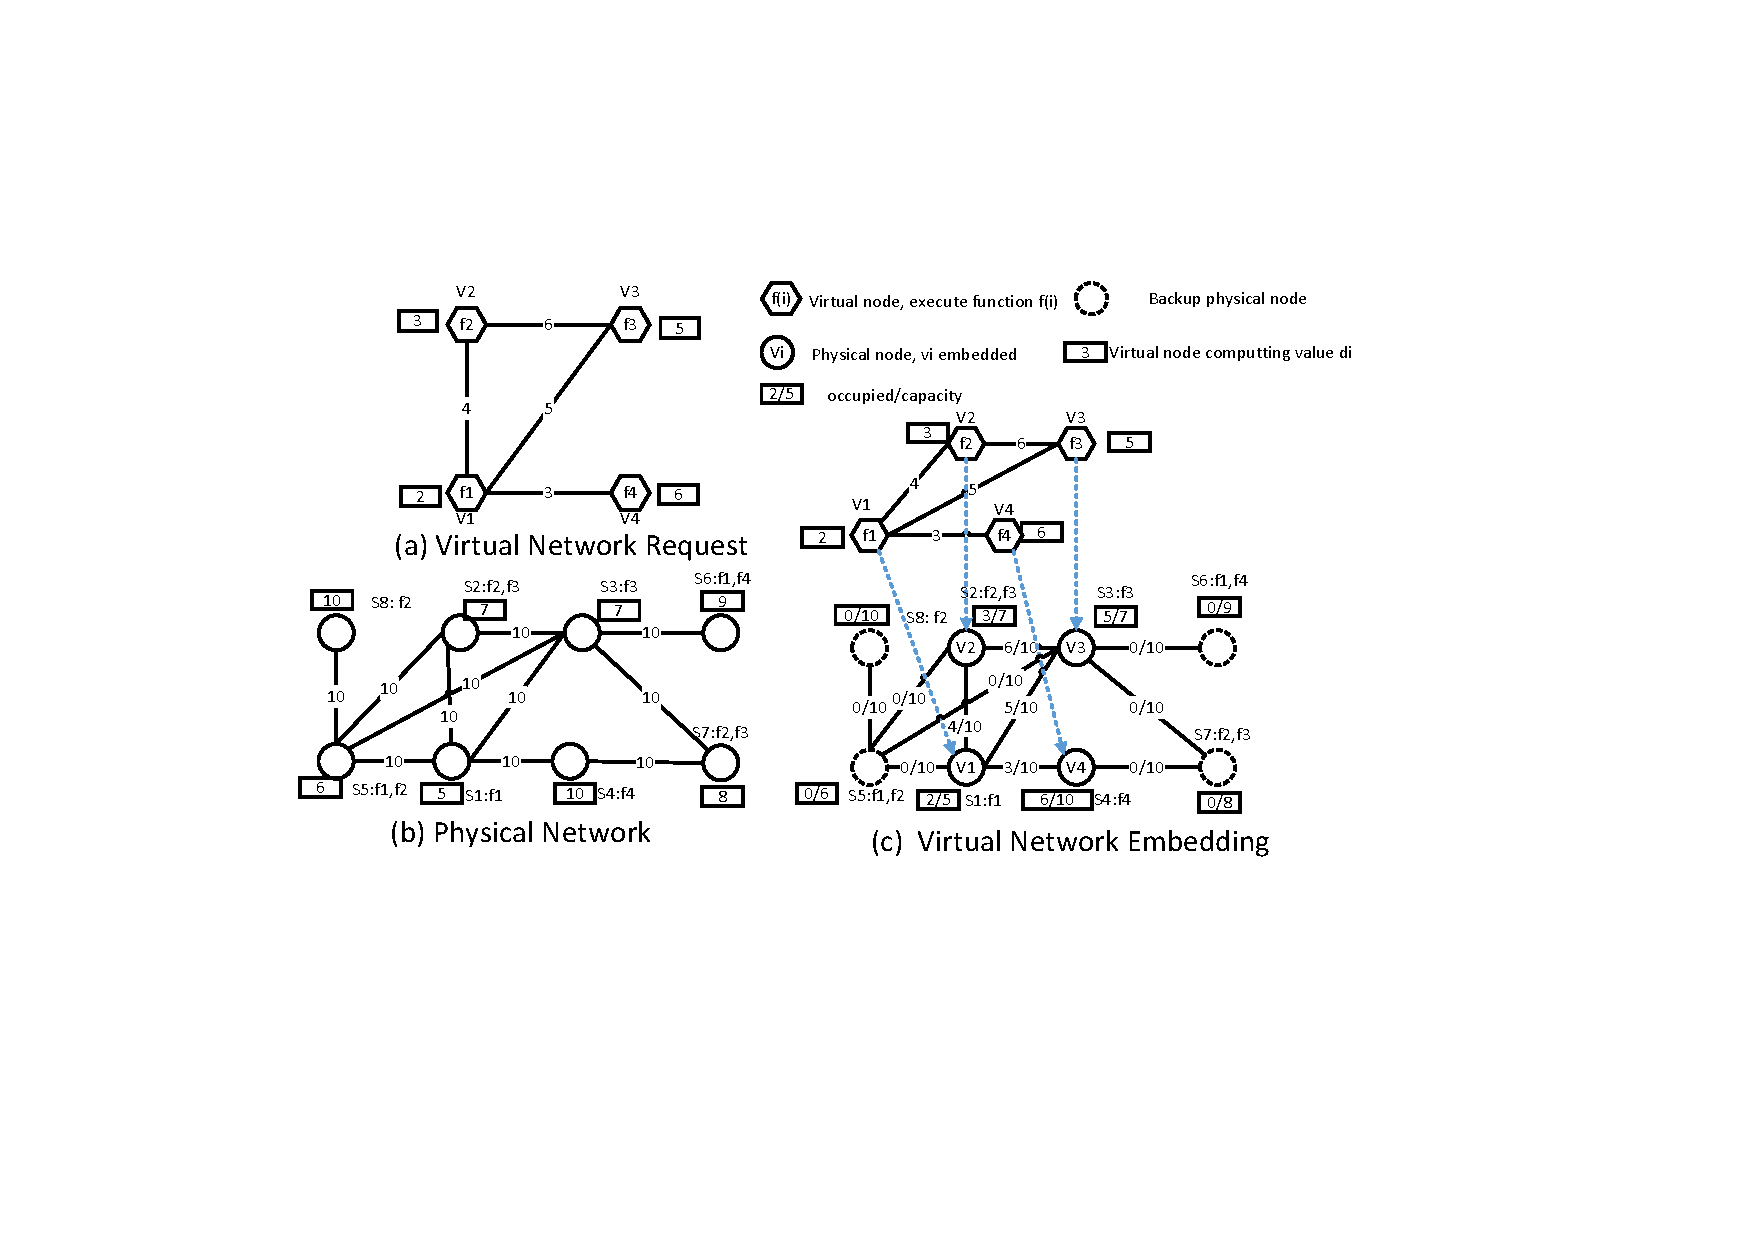
\includegraphics[width=5in]{Fig/VNQSNVNE}\\
\caption{(a) Virtual Network Request $G(V,E)$, $V=\{v_1,v_2,v_3,v_4\}$, $E=\{e_{12},e_{23},e_{13},e_{14}\}$,  $f(i)=\{f_1,f_2,f_3,f_4\}$, $d_i=\{2,3,5,6\}$, $d_{ij}=\{4,5,3,6\}. $(b) Physical Network $G(S,L), S=\{s_1,s_2,s_3,s_4,s_5,s_6,s_7,s_8\}, L=\{l_{12},l_{13},l_{14},l_{15},l_{23},l_{25},l_{35},l_{36},l_{37},l_{47},l_{58}\}, F(i)=\{\{f_1\},\{f_2,f_3\},\{f_3\},\{f_4\},\{f_1,f_2\},\{f_1,f_4\},\{f_2,f_3\},\{f_2\}\}, c_i=\{5,7,7,10,6,9,8,10\}, b_{ij}=\{10,10,10,10,10,10,10,10,10,10,10\}$ (c) Vertex mapping $v_1\rightarrow s_1, v_2\rightarrow s_2, v_3\rightarrow s_3, v_4\rightarrow s_4$, link mapping $e_{12}\rightarrow l_{12},e_{23}\rightarrow l_{23},e_{13}\rightarrow l_{13},e_{14}\rightarrow l_{14}$.}\label{fig:VNQSNVNE}
\end{figure*}


We model the \textbf{physical network} as an undirected graph $G (S,L)$, where $S$ and $L$ is the sets of physical nodes and physical links, respectively.
 For physical node  $s_i$, we use $F(i)$ and $c_i$ to respectively denote the set of feasible virtual functions can be executed on this node and the available computational capacity. Each physical link $l_{ij}$ has an available bandwidth of $b_{ij}$. In  the physical network in Fig.\ref{fig:VNQSNVNE}(b), physical node set $S=\{s_1,s_2,s_3,s_4,s_5,s_6,s_7,s_8\}$,  link set $L=\{l_{12},l_{13},l_{14},l_{15},l_{23},l_{25},l_{35},l_{36},l_{37},l_{47},l_{58}\}$, the  feasible virtual function set of each physical node is  $F(1)=\{f_1\}$, $F(2)=\{f_2,f_3\}$, $F(3)=\{f_3\}$, $F(4)=\{f_4\}$, $F(5)=\{f_1,f_2\}$, $F(6)=\{f_1,f_4\}$, $F(7)=\{f_2,f_3\}$,$F(8)=\{f_2\}$, respectively.



Given the VN request $G (V,E)$, the problem of \textbf{\emph{virtual network embedding}} aims to map this request onto the physical network $G (S,L)$ while providing enough resource as demanded. A feasible mapping should satisfy three constraints including node capacity constraint, link bandwidth constraint, and function type constraint.

For a virtual node $v_i$, a physical node $s_j$ can hold this virtual node only when both node capacity constraint  and  function type constraint (i.e., ${f_i} \in {F_j}$) are satisfied, that is, the node capacity request should be satisfied by the physical node with $d_i\leq c_j$, the virtual function required to be executed on  virtual node ${v_i}$ can be executed on physical node $s_j$ with ${f_i} \in {F_j}$. If a physical node $s_j$ satisfies both two  constraints, the node mapping is feasible, and we denote such mapping as $\phi ({v_i}) = {s_j}$.

%Denote the corresponding physical node that holds $v_i$ as $s_j$. Under node capacity constraint, we have $d_i\leq c_j$, that is, the node capacity request should be satisfied by the physical node. Besides capacity constraint, there is a location constraint should be satisfied on the physical node, that is, a virtual node ${v_i} \in V$ can only be provisioned on a physical node $s_j$ with ${f_i} \in {F_j}$. That is, the virtual function running on virtual node ${v_i}$ can be executed on physical node $s_j$. If a physical node $s_j$ satisfies both node capacity constraint and location constraint, the node mapping is feasible, and we denote such mapping as $\phi ({v_i}) = {s_j}$.

For a virtual link $e_{ij}$ with its two virtual nodes are mapped to two physical nodes $s_{i'}$ and $s_{j'}$ (i.e., $\phi({v_i}) = {s_{i'}}$ and $\phi({v_j}) = {s_{j'}}$). Under link bandwidth constraint, if $d_{ij}\leq b_{i'j'}$ where $b_{i'j'}$ is the  available bandwidth  of the path connecting the physical nodes $s_{i'}$ and $s_{j'}$, virtual link  $e_{ij}$ can be mapped to the physical path $p_{\phi({v_i}) \phi({v_j})}$, we denote the feasible link mapping as $\rho(e_{ij}) = p_{\phi({v_i}) \phi({v_j})}$.

Obviously, to find a feasible virtual network embedding, we should find two mapping functions $\phi$ and $\rho$ to map all the virtual nodes to physical nodes, and all the virtual links to physical paths.


Fig.\ref{fig:VNQSNVNE}(c) shows a feasible virtual network embedding to embed virtual network in Fig.\ref{fig:VNQSNVNE}(a) to the physical network in Fig.\ref{fig:VNQSNVNE}(b) where  virtual node $v_1$ is embedded in physical node $s_1$, virtual node $v_2$ is embedded in physical node $s_2$, virtual node $v_3$ is embedded in physical node $s_3$, and virtual  node $v_4$ is embedded in physical node $s_4$, respectively. In Fig.\ref{fig:VNQSNVNE}(C), we also show the resource occupied and available in the physical network after such mapping. For example, for physical node $s_1$, its occupied computation capacity is 2 and the available capacity is 5. %The virtual link $e_{12}$ is mapped to physical link $l_{12}$ , we also draw the occupied bandwidth and the available bandwidth along the physical link  $l_{12}$.


%, we embed virtual network request as shown in Fig.\ref{fig:VNQSNVNE}(A) into the substrate network, node $v_1$ is embedded in node $s_1$, node $v_2$ is embedded in node $s_2$, node $v_3$ is embedded in node $s_3$, node $v_4$ is embedded in node $s_4$.  node computing demand of every virtual node is not more than these virtual nodes corresponding substrate node's remain node computing. Every link of virtual network request exist a corresponding path consisted of substrate node and remain bandwidth of all links of corresponding path is more than demand  bandwidth of the virtual network link.


Given the VN request $G (V,E)$ and the physical network  $G (S,L)$, for a feasible mapping, we  denote the mapping physical graph as $G\left( {\hat S,P} \right)$ where $\hat S$ is the physical node set that hold the virtual nodes with $\hat S = \{ {s_{i'}}:\phi({v_i}) = {s_{i'}},for\ {\rm{ }}all\ {v_i} \in V,{s_{i'}} \in S\}$  and $P$ is the path set in which each holds one virtual link with $P = \{ p_{\phi({v_i}) \phi({v_j})}:\rho(e_{ij}) = p_{\phi({v_i}) \phi({v_j})}{\rm{ }}, for\ all,{e_{ij}} \in E\}$. As each virtual link corresponds a physical network path which consisting of multiple physical links, we also denote $G\left( {\hat S,\hat L} \right)$ as the occupying physical network with  $\hat L = \{ {l_{pg}}:{l_{pg}} \in {p_{s_{i'}s_{j'}}}, \rho(e_{ij}) = p_{\phi({v_i}) \phi({v_j})},for\ all\ {e_{ij}} \in E,{l_{pg}} \in L\}$.

 %only subset of $S$ and $L$ are involved to hold the virtual network. We denote the sub-graph as $G\left( {\hat S,\hat L} \right)$ where $\hat S$ is the subset of $S$ and $\hat L$ is the subset of $L$. Obviously, we have $\hat S = \{ {s_{i'}}:{v_i} \to {s_{i'}}{\rm{ }}for{\rm{ }}all{\rm{ }}{v_i} \in V,{s_{i'}} \in S\}$ and $\hat L = \{ {l_{pg}}:{l_{pg}} \in {p_{i'j'}},{e_{ij}} \to {p_{i'j'}}{\rm{ }}for{\rm{ }}all{\rm{ }}{e_{ij}} \in E,{l_{pg}} \in L\}$. We denote $G\left( {\hat S,\hat L} \right)$ as the occupying physical network of the virtual request. As ${e_{ij}} \to {p_{i'j'}}$, that is, each virtual link corresponding a path, we can also denote the mapping physical graph as $G\left( {\hat S,P} \right)$  where $P$ is the corresponding path sets in the process of the embedding mapping.




Lots of studies investigate the virtual network embedding problem \cite{fischer2013virtual}, as the focus of this paper is not virtual network embedding, we adopt algorithm in \cite{lischka2009virtual} as the basic virtual network embedding algorithm.
%There has existed most studies about virtual network embedding method listed in a survey paper\cite{fischer2013virtual}.


\subsection{Survivable virtual network embedding}
Due to malicious attacks, natural disasters, unintentional cable cuts, planned maintenance, equipment malfunctioning, physical nodes that host the virtual nodes may suffer unavoidable fail. Failure in the VN can happen when single or multiple physical network components failures, which results in financial losses. In general, the multiple physical node's simultaneous failure is mutual independent, a single node failure happen at most of time\cite{yeow2011designing}. In this paper, we study the survivable virtual network embedding problem with single node failure. In section, we will discuss how our algorithm can be extended to the scenario with multiple node failure.


For a VN request $G (V,E)$ and a physical network $G (S,L)$, given a feasible mapping with its occupying physical network $G\left( {\hat S,\hat L} \right)$, this paper wants to add minimum backup physical resources to  provide survivable network service when any one physical node fails.

\begin{figure}
\centering
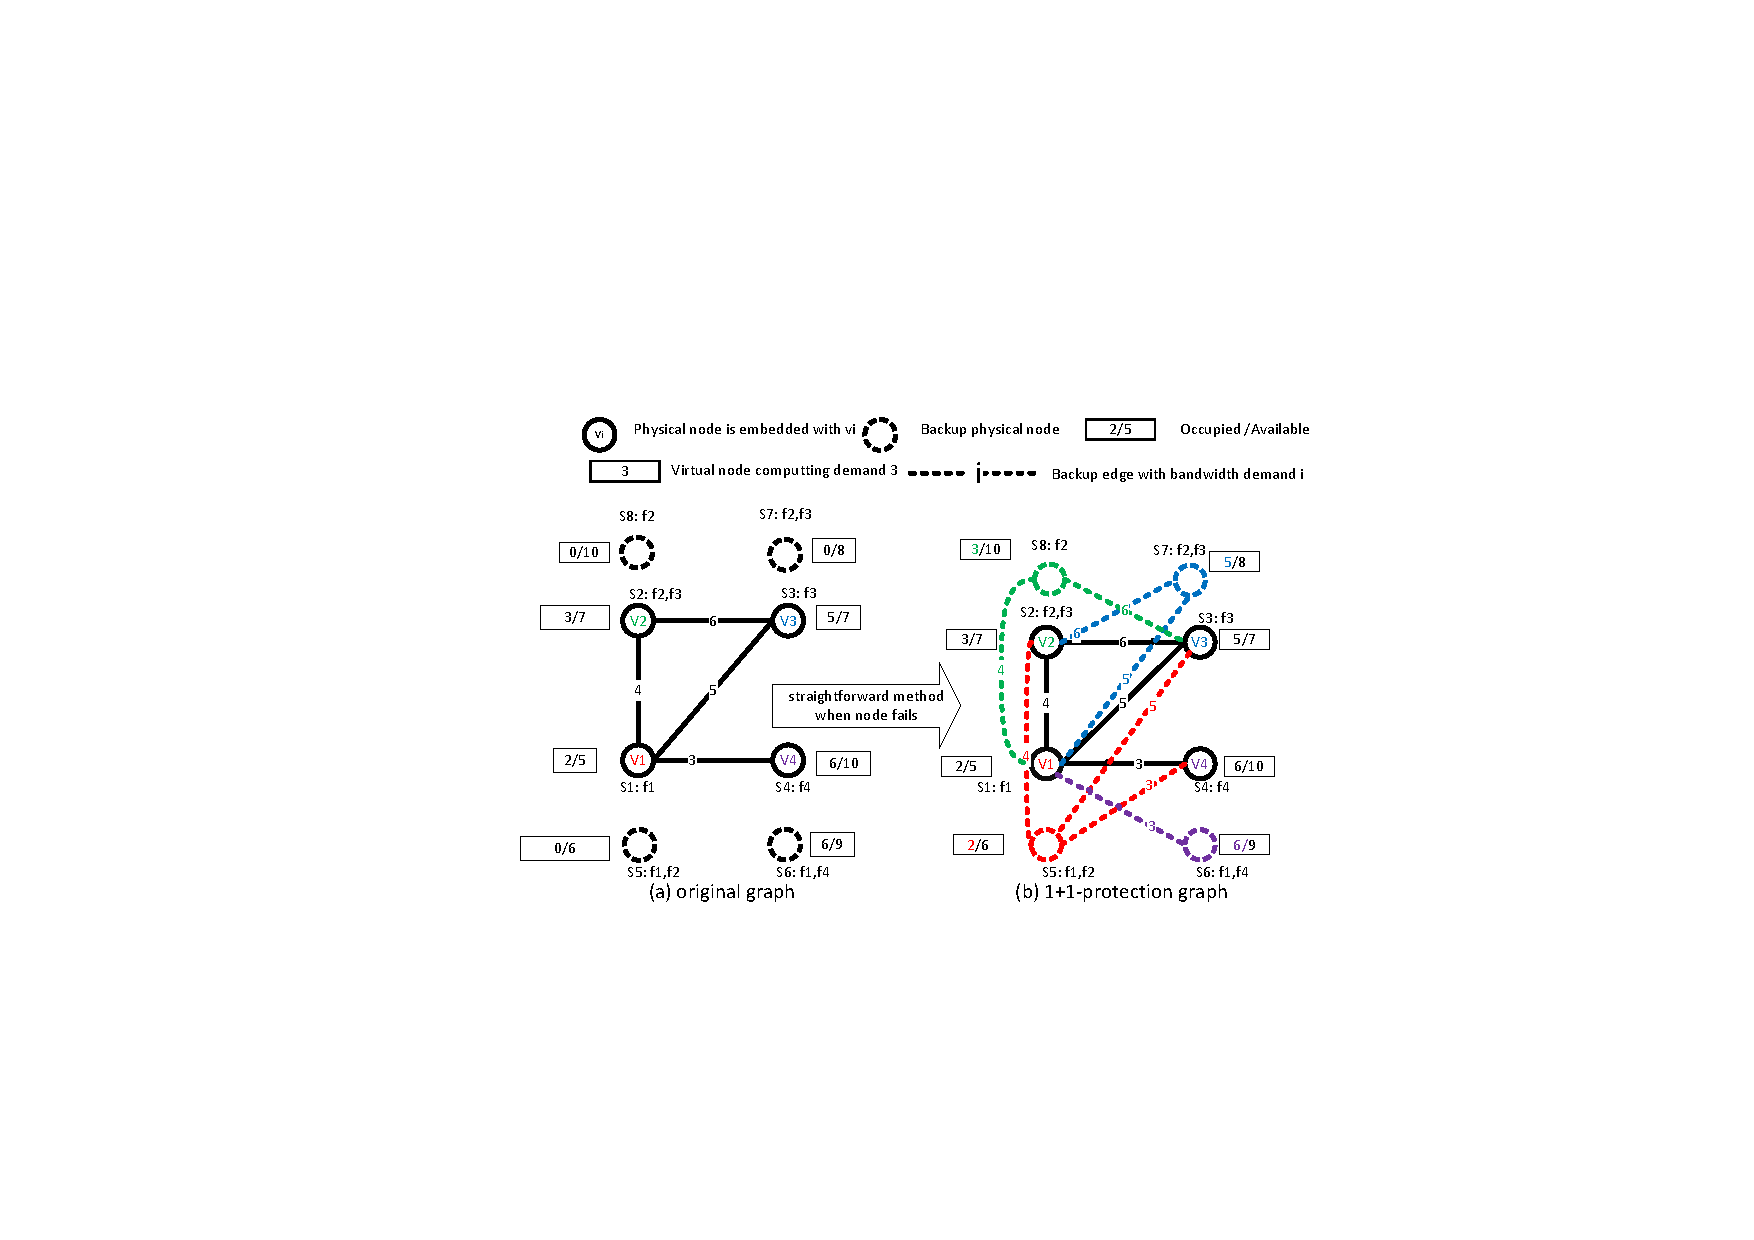
\includegraphics[width=3.5in]{Fig/One2OneProtection}\\
\caption{1+1-protection scheme}\label{fig:One2OneProtection}
\end{figure}

Node failures not only affect the visualized services running on the failed physical node, but also would terminate all the communications which traverse through this node. The fail of physical node $ {s_i} \in S $ results in the fail of physical links in ${L_i} = \left\{ {{l_{ik}}:k \in N(i)} \right\}$  where ${N(i)}$ is the neighbor nodes of node $ {s_i} $.

As we can not predict which node will fail even though we know multiple nodes will not simultaneously fail, to handle single node failure, one straightforward way  is to provision dedicated backup resource for each virtual node  in a VN request, also known as the 1 + 1-protection scheme.  Fig.\ref{fig:One2OneProtection} utilizes an example to illustrate this straightforward way. In the example, a virtual network with  4 virtual nodes are mapped to a physical network, where 4 physical nodes are involved in such embedding. To provide 1 + 1-protection scheme,  4 backup nodes, 8 backup links are added in the graph.

Although 1 + 1-protection scheme is simple to implement, it requires large amount of  backup resource. The aim of this paper is to provide survival network service with minimum backup resource cost.


%For example, when node $s_2$ fails, as it runs function $f_2$ for $v_2$ in the VN network, 1 backup node $s_8$ with $F(8)=\{f_2\}$ and 2 backup links $(s_8, s_1)$ and $(s_8, s_3)$ are added. \textbf{For other example, when node $s_1$ fails, as it runs function $f_1$ for $v_1$ in the VN network, one backup node $s_5$ with $F(5)=\{f_1,f_2\}$ and 3 backup links $(s_5, s_2)$,$(s_5, s_3)$ and $(s_5, s_4)$ are added.}.


%, some backup physical node and path should be added. We denote the backup physical node set and link set as $S_b$ and $L_b$.
%
%
%
%
%Survivable virtual network embedding should add  backup resources to guarantee that when a physical node $ {s_i} \in S $ fails, the remaining physical resource plus the backup resources (i.e., $G\left( {\hat S + {S_b} - \{ {s_i}\} ,\hat L + {L_b} - {L_i}} \right)$) can still support a feasible mapping.
%
%
%
%Therefore,  this paper wants to solve the survivable virtual network embedding problem by minimizing the additional resources needed when single node fails. Specially, given virtual network request $G(V,E)$ and its mapping on the physical network $G\left( {\hat S,\hat L} \right)$, add node  and link in the physical network with minimum cost so that when single node fails, the virtual network request $G(V,E)$ can be still satisfied.

\section{Graph decomposition based problem formulation}
Survivable virtual network embedding requires to add  backup resources to guarantee that when any one physical node  fails, the remaining physical resource plus the backup resources can still support a feasible mapping. To facilitate finding feasible mapping when node fails, this section first decomposes the virtual network and physical network into star based local components. Based on which, a novel   bipartite graph is proposed and the problem of survivable virtual network embedding with minimum backup resource is formulated as a virtual star assignment problem based on the well defined bipartite graph.


%with the edge weight  intelligently  denoting the backup resource cost to map virtual network components to the physical components. Based on the graph, the minimum backup cost Survivable virtual network embedding is modeled as a constrained multiple  knapsack problem which is proved to be NP-hard problem.
\subsection{Star based graph decomposition}


The virtual network is decomposed into virtual local stars. Each virtual local star associates with a virtual node. Given virtual node $v_i$, the corresponding virtual local star is defined as an attributed, single-level, rooted tree and expressed as

\begin{equation}
VirtualStar(v_i)=(v_i, \phi(v_i), d_i, f_i, D_i, N_i)
\label{eq:virtualstar}
\end{equation}

where $N_i$ is the neighbor node set of $v_i$ in the virtual network and ${D_i}$ denotes the bandwidth demand set associate with node $v_i$ with ${D_i} = \left\{ {{d_{ij}}|{v_j} \in {N_i}} \right\} $.
Note that, VirtualStar($v_i$) includes the node mapping information $\phi(v_i)$. As we want to minimize the backup resource to provide the survivable network service, re-use the mapping before node failure may be a good choice to reduce the additional resource and make the system remain stable. In the virtual star structure, edges exist between the root node and its neighbor nodes, and no edge exists among its neighbor nodes.

The physical network is decomposed into physical local stars. Similarly, each physical local star associates with a physical node. Given physical node $s_j$, the corresponding physical local star is defined as an attributed, single-level, rooted tree and expressed as

\begin{equation}
PhysicalStar(s_j)=(s_j, \phi^{-1}( s_j), c_j, F(j), \phi(N(\phi^{-1}( s_j))), a)
\label{eq:physicalstar}
\end{equation}

where $\phi^{-1}( s_j) $ is the virtual nodes that map to physical node $s_j$, $N(\phi^{-1}( s_j))$ is the neighbor nodes of the virtual nodes in $\phi^{-1}( s_j)$, $\phi(N(\phi^{-1}( s_j)))$ is the physical nodes that hold these neighbors, $c_j$ is the node capacity, $F(j)$ is the virtual functions supported by $s_j$,  $a$ is a one-bit single with its value being 0 or 1 to indicate whether this physical node has setup the virtual machine. Similarly to virtual star, in the physical star structure, edges exist between the root node and its neighbor nodes, and no edge exists among its neighbor nodes.

Virtual star and physical star defined in (\ref{eq:virtualstar}) and (\ref{eq:physicalstar})  well capture the local structures hidden in the VN request to preserve the relationship of node with its adjacent.

Based on the virtual local star and physical virtual star, the virtual network and physical network can be decomposed into multiple components.
\subsection{Bipartite graph}
We build a bipartite graph $G=\{V_1,V_2,E\}$ to present the relationship between the virtual network and physical network.
$V_1$ and $V_2$ are the vertex sets  representing the set of virtual stars and the set of physical stars, respectively. If VirtualStar($v_i$)'s virtual function $f_i$ can be executed by a physical node $s_j$ with ${f_i} \in {F_j}$, an edge $e(i,j)$ is added to the edge set $E$ to connect the VirtualStar($v_i$) and PhysicalStar($s_j$).

Our goal is to minimize the backup resource to provide survivable service. To serve the goal, given edge $e(i,j)$, we define the edge weight $w(i,j)$  as the backup resource cost to map the virtual star($v_i$) to the physical star ($s_j$) when  node failure happens. According to whether the virtual node $v_i$ is mapped to the physical node $s_j$ before node fails, we define the edge weight in two different cases.

\begin{equation}
\footnotesize
w(i,j) = \left\{ {\begin{array}{*{20}{c}}
   { \alpha \sum\limits_{\phi ({v_k}) \notin \phi (N({\phi ^{ - 1}}({s_j})))} {{d_{ik}}} } & {{v_i} \in {\phi ^{ - 1}}({s_j}),v_k \in N(i)}  \\
   {\alpha \sum\limits_{k \in N(i)} {{d_{ik}}}  + \beta {M_m} + \lambda {c_i} + \theta } & {{v_i} \notin {\phi ^{ - 1}}({s_j}),v_k \in N(i)}  \\
\end{array}} \right.
\label{eq:edge weight}
\end{equation}
In (\ref{eq:edge weight}), $\theta$ is defined as follows.
\begin{equation}
\theta  = \left\{ {\begin{array}{*{20}{c}}
   {{C_s}} & {a = 0}  \\
   0 & {a = 1}  \\
\end{array}} \right.
\end{equation}
In the first case (${v_i} \in {\phi ^{ - 1}}({s_j})$), as the virtual node $v_i$ is mapped to the physical node $s_j$ before node fails, node capacity demand is satisfied already, thus only bandwidth backup cost is needed when map the virtual star ($v_i$) to the physical star ($s_j$). For each neighbor $v_k \in N(i)$ , if  the physical node that holds virtual node $v_k$ fails with ${\phi ({v_k}) \notin \phi (N({\phi ^{ - 1}}({s_j})))}$, new path with bandwidth $d_{ik}$ should be added as the backup resource. Therefore, in this case, the backup cost only includes bandwidth cost and expressed as $ { \alpha \sum\limits_{\phi ({v_k}) \notin \phi (N({\phi ^{ - 1}}({s_j})))} {{d_{ik}}} }$ where $\alpha$ is the unit bandwidth cost.

In the second case (${v_i} \notin {\phi ^{ - 1}}({s_j})$), as the virtual node $v_i$ is not mapped to the physical node $s_j$ before node fails,  virtual node $v_i$ needs to be migrated to physical node $s_j$. Therefore, the edge weight $w(i,j)$ includes node��s capacity cost, path��s bandwidth cost, and migration cost to migrate a virtual node from a physical node to another physical node when physical nodes fail. Moreover, if the backup physical node $s_j$ does not  hold any virtual node before, migrating a virtual node to this physical node also introduces a \text{virtual machine booting  cost} denoted as $C_s$.




Fig.\ref{fig:StarRepresentation} shows one example of such  bipartite graph when physical node $s_1$ fails. The edge weight of this   bipartite graph can be shown in  Eq(\ref{lab:Node1FaliureAlignmentMatrixNew}).
\begin{figure}
\centering
% Requires \usepackage{graphicx}
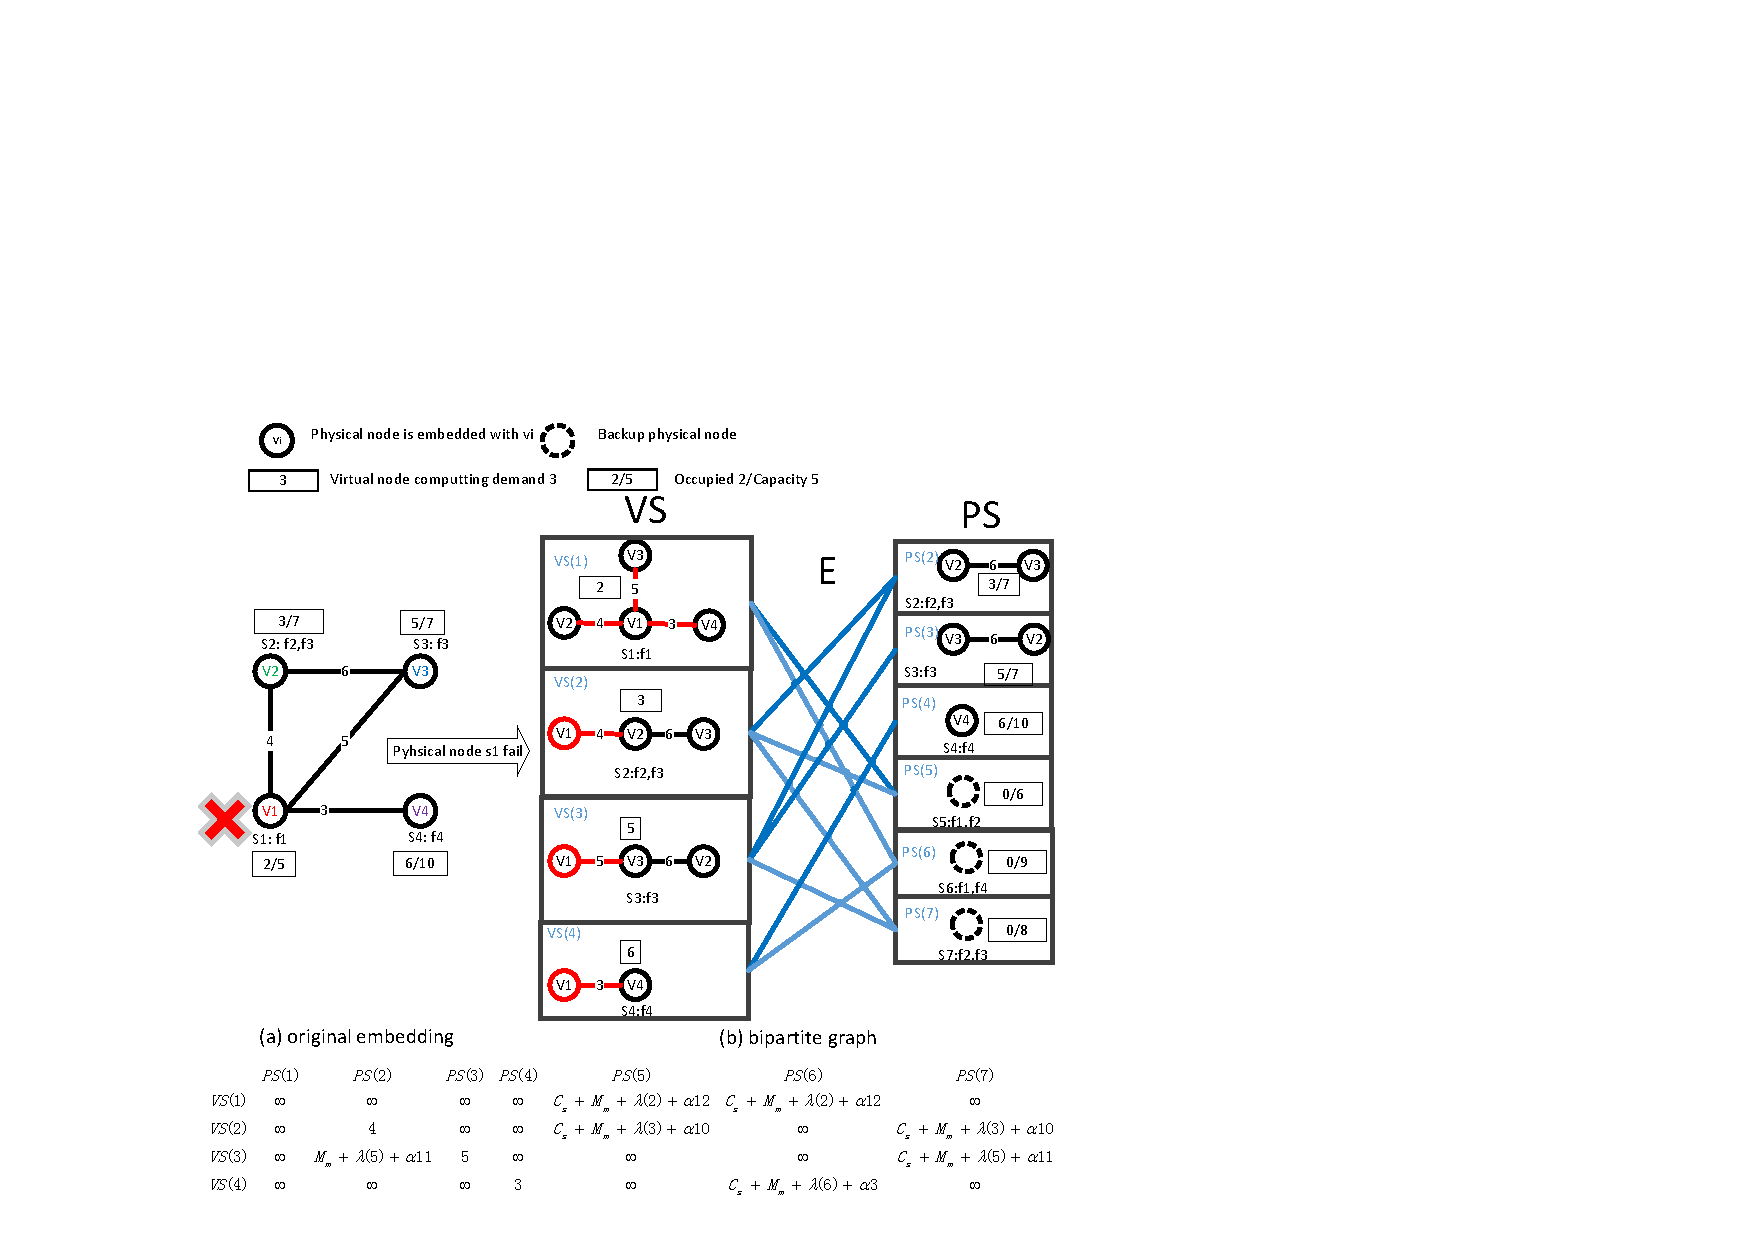
\includegraphics[width=3.7in]{Fig/StarRepresentation}\\
  \caption{Components of VirtualStar($v_i$) and PhysicalStar($s_j$) when physical node $s_1$ fail}\label{fig:StarRepresentation}
\end{figure}

\begin{equation*}
\tiny{
 {\begin{array}{*{20}{c}}
&R_{S_{1}}&R_{S_{2}}&R_{S_3}&R_{S_4}&R_{S_5}&R_{S_6}&R_{S_{7}}\\
{L_{V_1}}&\infty&\infty&\infty&\infty&\fbox{$C_{s}+M_{m}$+(2)+12}&C_{s}+M_{m}+(2)+12&\infty\\
L_{V_2}&\infty&\fbox{4}&\infty&\infty&C_{s}+M_{m}+(3)+10&\infty&C_{s}+M_{m}+(3)+10\\
L_{V_3}&\infty&M_{m}+(5)+11&\fbox{5}&\infty&\infty&\infty&C_{s}+M_{m}+(5)+11\\
L_{V_4}&\infty&\infty&\infty&\fbox{3}&\infty&C_{s}+M_{m}+(6)+3&\infty\\
\end{array}}
}
\label{lab:Node1FaliureAlignmentMatrixNew}
\end{equation*}


%\begin{equation*}
%\tiny{
% {\begin{array}{*{20}{c}}
%&{L_{V_1}}&L_{V_2}&L_{V_3}&L_{V_4}\\
%R_{S_{1}}&\infty&\infty&\infty&\infty\\
%R_{S_{2}}&\infty&\fbox{4}&M_{m}+(5)+11&\infty\\
%R_{S_{3}}&\infty&\infty&\fbox{5}&\infty\\
%R_{S_{4}}&\infty&\infty&\infty&\fbox{3}\\
%R_{S_{5}}&\fbox{$C_{s}+M_{m}$+(2)+12}&C_{s}+M_{m}+(3)+10&\infty&\infty\\
%R_{S_{6}}&C_{s}+M_{m}+(2)+12&\infty&\infty&C_{s}+M_{m}+(6)+3\\
%R_{S_{7}}&\infty&C_{s}+M_{m}+(3)+10&C_{s}+M_{m}+(5)+11&\infty\\
%\end{array}}
%}
%\label{lab:Node1FaliureAlignmentMatrixNew}
%\end{equation*}





For the virtual node $v_i$, if its virtual function can not be executed in physical node $s_j$
with $f(i) \notin F(i)$, no edge is connected with $VirtualStar(v_i)$ in $V_1$ and $PhysicalStar(s_j)$ in $V_2$. To facilitate problem formulation in following section, we set the edge weight to be $\infty $. For example, as $v_1$'s virtual function is $f_1$, it can not be executed in physical node $s_2$. Therefore, no edge is added to connected with $VirtualStar(v_1)$ in $V_1$ and $PhysicalStar(s_2)$ in $V_2$ and we set the $w(1,2)=\infty$.

For $VirtualStar(v_2)$, as $v_2$ is originally hold by $s_2$, however, when physical node $s_1$ (which holds $v_1$ originally) fails, the virtual link $e_{12}$ fails to be mapped to the physical network. We should find a new path connecting   $\phi(v_2)$ with $\phi(v_1)$ satisfying bandwidth demand  $d_{12}=4$. Therefore, the edge weight connecting $VirtualStar(v_2)$ and $PhysicalStar(s_2)$ is 4.

When node $s_1$ fails, it directly impact virtual node $v_1$. As $s_5$ can execute virtual function $f_1$, we can add a edge to  connect $VirtualStar(v_1)$ and $PhysicalStar(s_5)$. However, in this example, as $s_5$ does not setup virtual machine before, there also introduces virtual machine's start cost $C_s$.  Therefore, the link weight is $C_s$ (start cost)+ $M_m$ (migrating cost)+ $3$ (node capacity cost)+ $10$ (bandwidth cost).

\subsection{Problem formulation}
To provide survivable service, each virtual star (both the root virtual node and the virtual links connecting root node and its adjacent nodes) should be mapped to a physical star.
Assume virtual network consists of $n$ virtual nodes, thus $n$ virtual stars. The physical network consists of $m$ physical nodes, thus $m$ physical stars. In Eq(\ref{eq:indication}), we use bit binary $M_{ij}$ to denote whether  the $i$-th virtual star is mapped to the $j$-th physical star.
\begin{equation}
{M_{ij}} = \left\{ {\begin{array}{*{20}{c}}
   1 & {map \ virtualstar(i) \  to  \ physicalstar(j)}  \\
   0 & {otherwise}  \\
\end{array}} \right.
\label{eq:indication}
\end{equation}
When a physical node fails, to minimize the backup resource cost, the survivable virtual network embedding problem can be defined as follows.
\begin{equation}
\begin{array}{*{20}{c}}
   {\mathop {\min }\limits_{{M_{ij}}} } & {\sum\limits_{i = 1}^n {\sum\limits_{j = 1}^m {{M_{ij}}{w_{ij}}} } }  \\
   {s.t.,} & {\sum\limits_{i = 1}^n {{d_i}{M_{ij}}}  \le {c_j}}  \\
   {} & {\sum\limits_{j = 1}^m {{M_{ij}}}  \le 1}  \\
   {} & {{M_{ij}} = \{ 0,1\} }  \\
\end{array}
\label{eq:problem formulation}
\end{equation}
where ${\sum\limits_{i = 1}^n {\sum\limits_{j = 1}^m {{M_{ij}}{w_{ij}}} } }$ denotes the total backup resource  cost to map all the virtual stars to physical stars when physical nodes fails.  In (\ref{eq:problem formulation}), ${\sum\limits_{i = 1}^n {{d_i}{M_{ij}}}  \le {c_j}}$ is the physical node's capacity constraint, that is, even though multiple virtual nodes are allowed to be mapped to a physical node, the total capacity demand should not be larger than the capacity of the physical node. ${\sum\limits_{j = 1}^m {{M_{ij}}}  \le 1}$ indicates that one virtual star can be mapped to only one physical star.

Obviously, problem defined in (\ref{eq:problem formulation}) is an binary ILP problem, which is general an NP-complete problem according to Karp's 21 NP-complete problems\cite{karp1975computational}. %In following  Theorem 1, we validate the theorem.

\textbf{Theorem 1} Problem defined in (\ref{eq:problem formulation}) is an NP-complete problem.
\begin{proof}
If  there is only one physical node with $m=1$, our survivable virtual network embedding problem can be  degenerate into single knapsack problem, which is NP-complete problem. In practice, $m$ is usually larger than 1, single knapsack problem is subproblem of survivable virtual network embedding problem and given a feasible solution is easily verified in polynomial time, according to the reducibility theorem\cite{wood1987theory} in computer complexity field, it is easy to conclude that our defined in (\ref{eq:problem formulation}) is also NP-complete.
\end{proof}

\subsection{Dynamic Programming Mehtod}
\label{lab:DynamicProgrammingEquation}

Although solving the ILP formulation will result in a minimum cost survival virtual network embedding, its exponential time complexity makes such approach impractical to embed a virtual network to a large  physical network. In this section, we propose a dynamic programming based algorithm that has only a polynomial time complexity and, thus, is feasible for practical network systems.


To describe our dynamic programming based algorithm, we define  $dp[i][{x_1}][{x_2}] \ldots [{x_m}]$ to denote the best virtual star placement with the minimum backup resource cost to place the first $i$ ($0 \le i \le n $) virtual stars to the $m$ physical stars with their capacity  limit being $ x_1$, $ x_2$, $\ldots$, $x_m$ in the physical network.

The $i$-th virtual node star has the options to  be placed onto any one of the physical stars that are alive. Let $\theta (i,j)$ denote the backup resource cost to place the $i$-th virtual node star to the $j$-th physical node after the first $i-1$ virtual nodes are best placed. $\theta (i,j)$ is expressed as follows.
\begin{equation}
\footnotesize
\theta (i,j) = \left\{ {\begin{array}{*{20}{c}}
{dp[i - 1][x_1][{x_2}] \ldots [{x_j} - {d_i}] \ldots [{x_m}] + {w_{ij}}}\\
\infty
\end{array}} \right.\begin{array}{*{20}{c}}
{({x_j} \ge {d_i},{f_i} \in {F_j})}\\
{otherwise}
\end{array}
\label{eq:place i to j}
\end{equation}
In (\ref{eq:place i to j}), if the capability limit of the  physical node $x_j$ is large than the capacity demand $d_i$ and the virtual function $f_i$ can be executed in the physical node ${f_i} \in {F_j}$,  $\theta (i,j)$ is the sum of   the cost under best virtual star placement to place the first $i-1$ ($0 < i \le n $) virtual stars to the $m$ physical stars  (i.e., $dp[i-1][{x_1} - {d_i}][{x_2}] \ldots [{x_m}]$) and the cost that mapping the virtual star ($v_i$) to physical star ($s_1$) (i.e., $w_{i1}$ ).

Based on $\theta (i,j)$, $dp[i][{x_1}][{x_2}] \ldots [{x_m}]$ can be calculated through following dynamic programming function.
\begin{equation}
dp[i][{x_1}][{x_2}] \ldots [{x_m}] = min\{\theta (i,1),\theta (i,2),\ldots,\theta (i,j),\ldots,\theta (i,m)\}
\label{eq:update function}
\end{equation}


\begin{algorithm}
\label{alg:DPAlg}
\caption{Dynamic Programming Based Algorithm}
\begin{algorithmic}[1]
\REQUIRE {$dp[i][{x_1}][{x_2}] \ldots [{x_m}]=0(1\leq i \leq n, 0\leq x_1\leq c_1, 0\leq x_2\leq c_2,\ldots, 0\leq x_m\leq c_m)$ is firstly assigned as infinity $\infty$, $dp[0][{x_1}][{x_2}] \ldots [{x_m}]=0(0\leq x_1\leq c_1, 0\leq x_2\leq c_2,\ldots, 0\leq x_m\leq c_m)$, m is the number of physical nodes. $M[{x_1}][{x_2}] \ldots [{x_m}]=\textbf{0}_{n\times m}$ is placement of every virtual node.}
\ENSURE {obtaining optimal virtual node's placement when node up-bound capacity of physical nodes is $c_1,c_2,\ldots,c_m$, respectively.}
\FORALL{$i$ such that $1\leq i\leq n$ }
\FORALL{$x_1,x_2,\ldots,x_m$ such that $ c_1\geq x_1\geq d_i$, $c_2\geq x_2\geq d_i$,$c_3\geq x_3\geq d_i$,$c_m\geq x_m\geq d_i$}

\STATE {$dp[i][{x_1}][{x_2}] \ldots [{x_m}] = min\{\theta (i,1),\theta (i,2),\ldots,\theta (i,j),\ldots,\theta (i,m)\}$}

\STATE{$j' = \mathop {\arg \min }\limits_j \{\theta (i,1),\theta (i,2),\ldots,\theta (i,j),\ldots,\theta (i,m)\}$, }.
\STATE{$M[{x_1}][{x_2}] \ldots [{x_m}]=M[{x_1}][{x_2}] \ldots[x_{j'}-d_i]\ldots [{x_m}]$}
\STATE{$M[{x_1}][{x_2}] \ldots [{x_m}]_{ij'}=1$}
\ENDFOR
\ENDFOR
\RETURN $dp[i][{c_1}][{c_2}] \ldots [{c_m}]$ and $M[{c_1}][{c_2}] \ldots [{c_m}]$
\end{algorithmic}
\end{algorithm}

%\left[ {\begin{array}{*{20}{c}}
%0&0&0&0&0&0&0\\
%0&0&0&0&0&0&0\\
%0&0&0&0&0&0&0\\
%0&0&0&0&0&0&0
%\end{array}} \right]
The pseudo-code of the dynamic programming based algorithm is shown in Alg.\ref{alg:DPAlg}.
We further use an example in Fig.\ref{fig:DPIllustration} to illustrate the algorithm.

For clear presentation, in this example, three virtual stars needed to be placed to two available physical stars to achieve the minimum backup resource cost. The available capacity under physical nodes are $c_1=5$ and $c_2=4$, respectively. The capacity demands of these three virtual stars are $d_1=2$, $d_2=1$, and $d_3=2$. The virtual functions required to be executed in these virtual stars are $f(1)=f_1$, $f(2)=f_1$, $f(3)=f_2$. The functions supported by these two physical nodes are $F(1)=\{f_1,f_2\}$ and $F(2)=\{f_1\}$.

In Fig.\ref{fig:DPIllustration}, $x$ and $y$ axis denote the capacity limit of physical star $s_1$ and $s_2$, respectively. The  weight of edge connecting virtual stars to physical stars are $w_{11}=1$, $w_{12}=2$, $w_{21}=3$, $w_{22}=1$, $w_{31}=1$, $w_{32}=\infty$, respectively.


Initially, in Fig.\ref{fig:DPIllustration}(a), as no virtual star is placed to any physical stars, the backup cost under all the capacity limit cases ($x_1$=0,1,2,3,4 and $x_2$=0,1,2,3,4,5) are all 0. Specially, even though capacity limits are set 4 and 5, dp[0][4][5]=0.

In Fig.\ref{fig:DPIllustration}(b), when place the first virtual node $v_1$ with capacity demand $d_1=1$ to these two physical nodes, as $f_1$ can be executed in both physical nodes. Therefore, we have
\begin{equation}
dp[1][{x_1}][{x_2}] = \min \{\theta (1,1),\theta (1,2)\}
\end{equation}
Specially, if the capacity limit of these two physical nodes are $x_1$=2 and $x_2$=0, we have $dp[1][2][0]= dp[0][0][0]+w_{11}=2$. If the capacity limit of these two physical nodes are $x_1$=2 and $x_2$=4, we have $\theta (1,1)=dp[0][0][2]+w_{11}$ and $\theta (1,2)=\infty$ and thus $dp[1][2][4]=min\{ dp[0][0][4]+w_{11}), dp[0][2][2]+w_{12} \}=1$.

Similarly, when place the second virtual node with capacity demand $d_2=2$ to these two physical nodes, the cost results under all capacity limits is shown in Fig.\ref{fig:DPIllustration}(d). As $f_2$ can be executed in both physical nodes, thus $v_2$ can be placed into both physical nodes, we have
\begin{equation}
dp[2][{x_1}][{x_2}] = \min \{\theta (2,1),\theta (2,2)\}
\end{equation}
Specially, if the capacity limit of these two physical nodes are $x_1$=3 and $x_2$=4, we have $dp[2][3][4]=min\{dp[1][2][4]+w(2,1), dp[1][3][3]+w(2,2)\}=2$. If the capacity limit of these two physical nodes are $x_1$=3 and $x_2$=0, we have $dp[2][3][0]=dp[1][2][0]+w(2,1)=4$.

Fig.\ref{fig:DPIllustration}(d) shows the minimum resource cost result  when  place the third virtual node with capacity demand $d_3=1$ to these two physical nodes. As $f_3$ can only be executed in physical node $s_1$, we have $\theta (3,2)=\infty$. Specially, if the capacity limit of these two physical nodes are $x_1$=5 and $x_2$=0, we have $dp[3][5][0]=dp[2][3][0]+w(3,1)=4$. As the node capability of these two physical nodes are 5 and 4, respectively, we have $dp[3][5][4]=dp[2][3][4]+w(3,1)=3$, as indicted in Fig.\ref{fig:DPIllustration}(d), the best placement is achieved at dp[3][5][4]=3 with the assignment $v_1\rightarrow s_1, v_2\rightarrow s_2, v_3\rightarrow s_1$.

For example, as shown in Fig.\ref{fig:StarRepresentation} and Equ.(\ref{lab:Node1FaliureAlignmentMatrixNew}), the optimal $M_{ij}=\left[ {\begin{array}{*{20}{c}}
0&0&0&0&1&0&0\\
1&0&0&0&0&0&0\\
0&1&0&0&0&0&0\\
0&0&1&0&0&0&0
\end{array}} \right]$.

\begin{figure}
\centering
% Requires \usepackage{graphicx}
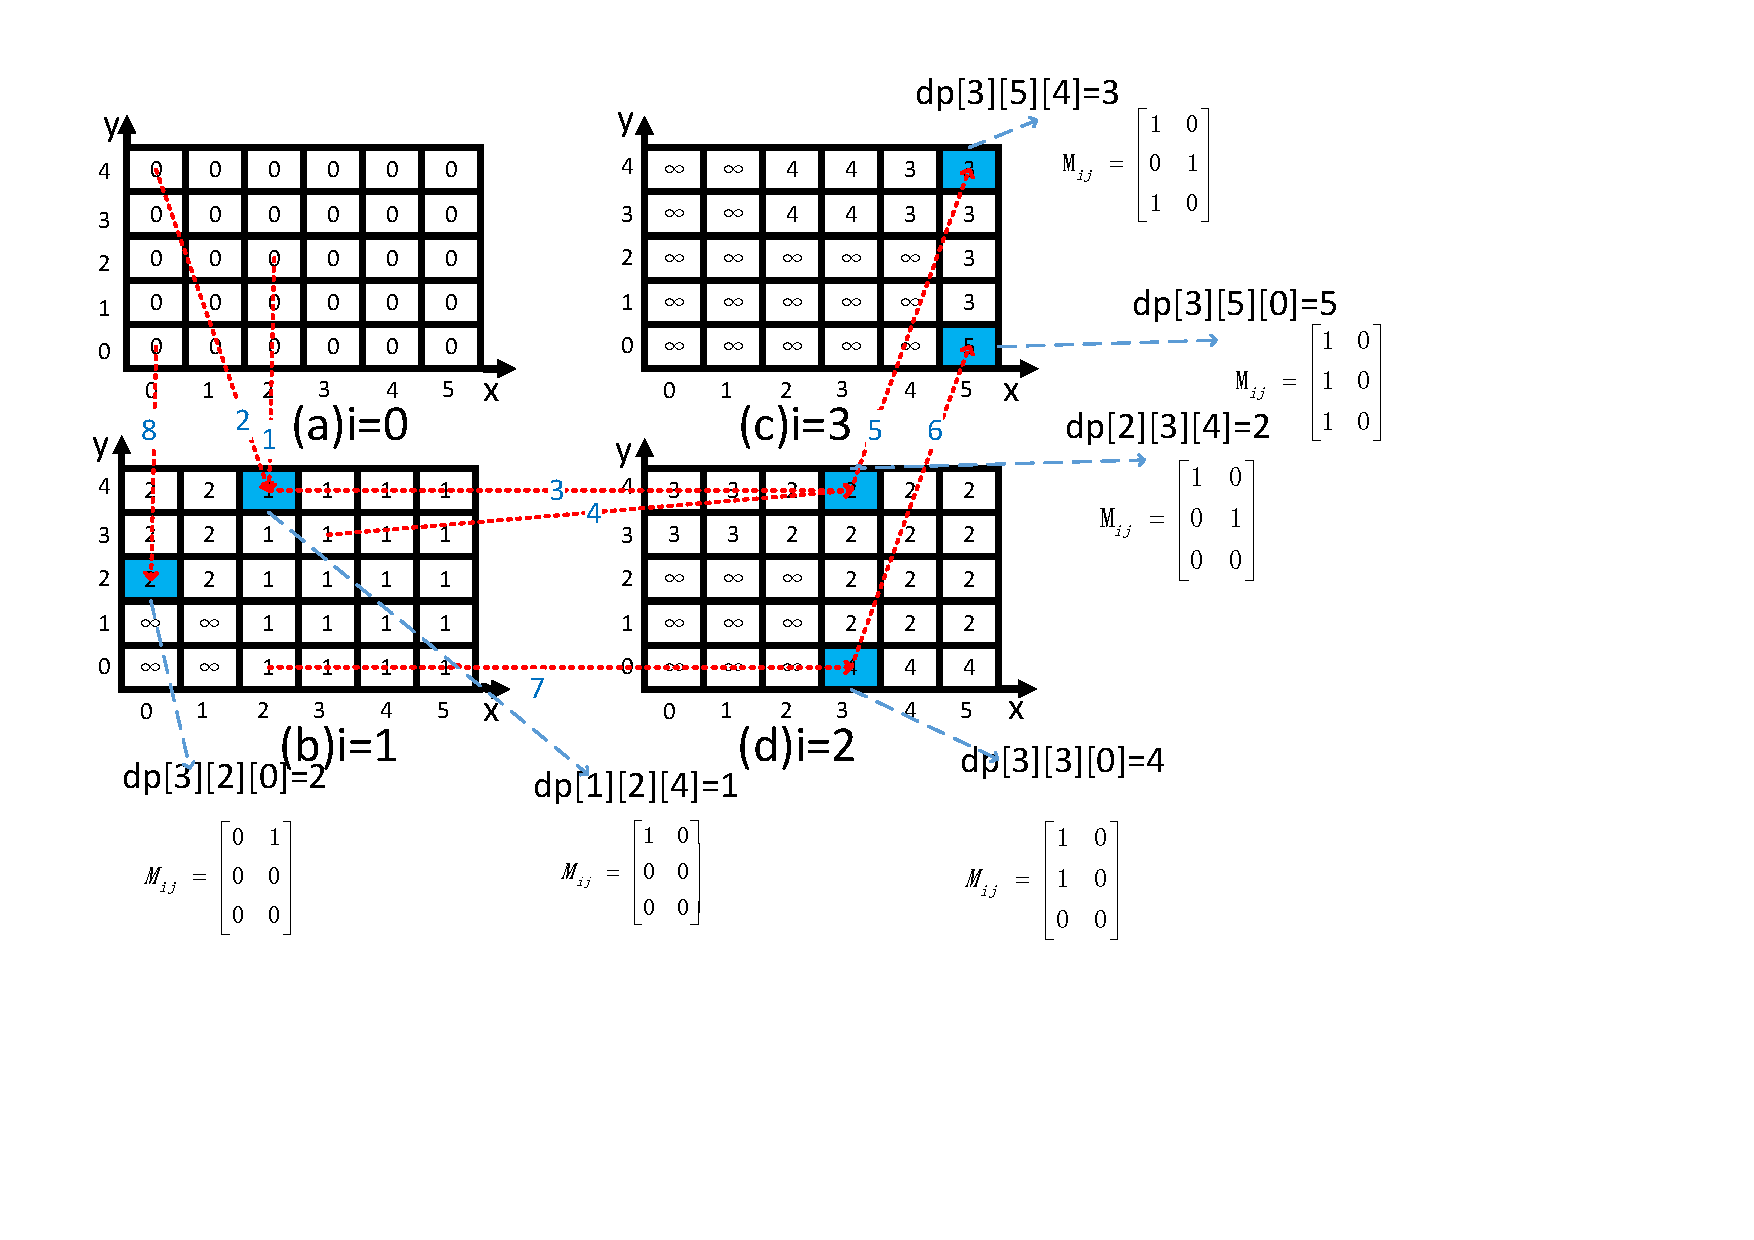
\includegraphics[width=4in]{Fig/DPIllustration}\\
  \caption{Three virtual node, the first virtual node could be placed to first and second physical node,  the second virtual node could be placed to first and second physical node,  the third virtual node could only be placed to first physical node.  The  node computation capacity of first physical node is 5, the node computation capacity of second physical node is 4. $w_{ij}$=[1,2;3,1;1,$\infty$].}\label{fig:DPIllustration}
\end{figure}




\begin{figure}
\centering
% Requires \usepackage{graphicx}
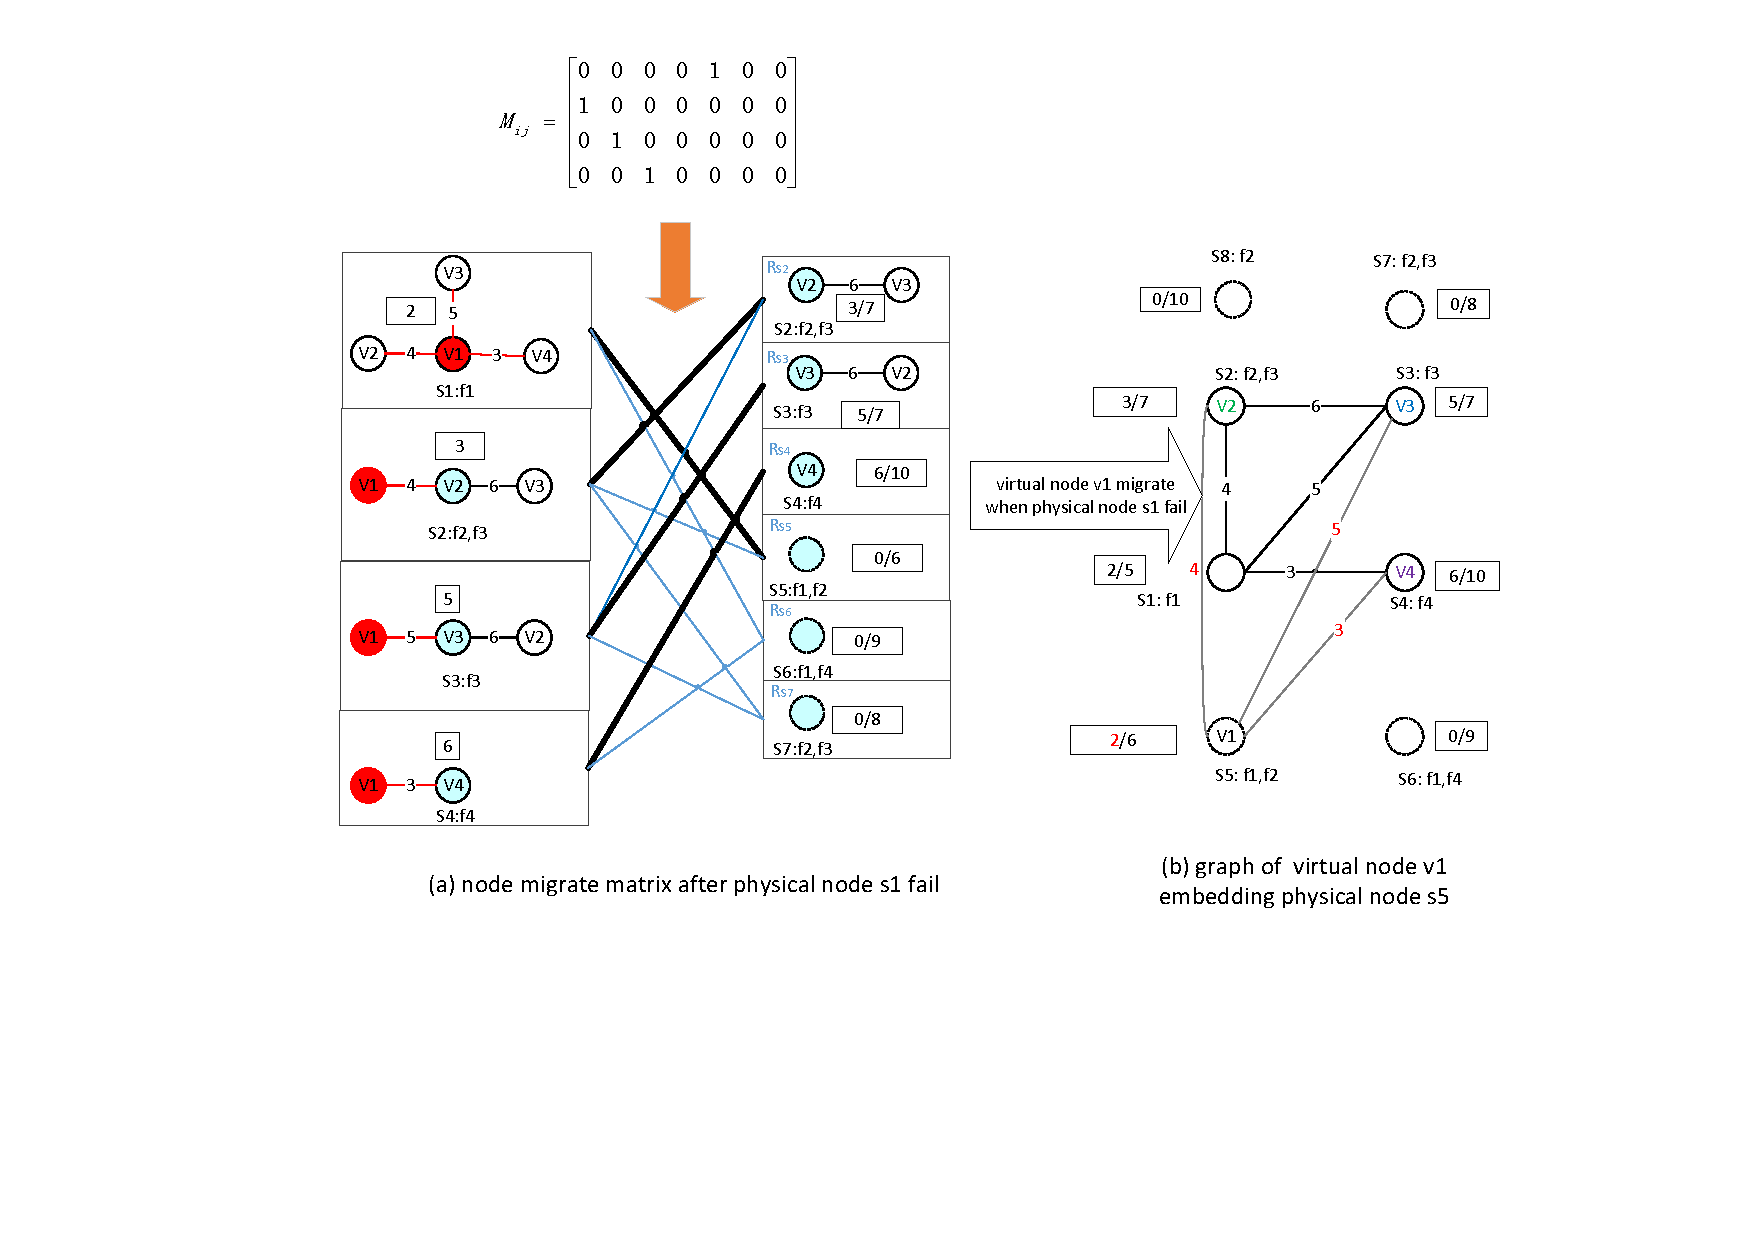
\includegraphics[width=4in]{Fig/Node1Failure}\\
  \caption{Node1Failure}\label{fig:Node1Failure}
\end{figure}

\begin{figure}
\centering
% Requires \usepackage{graphicx}
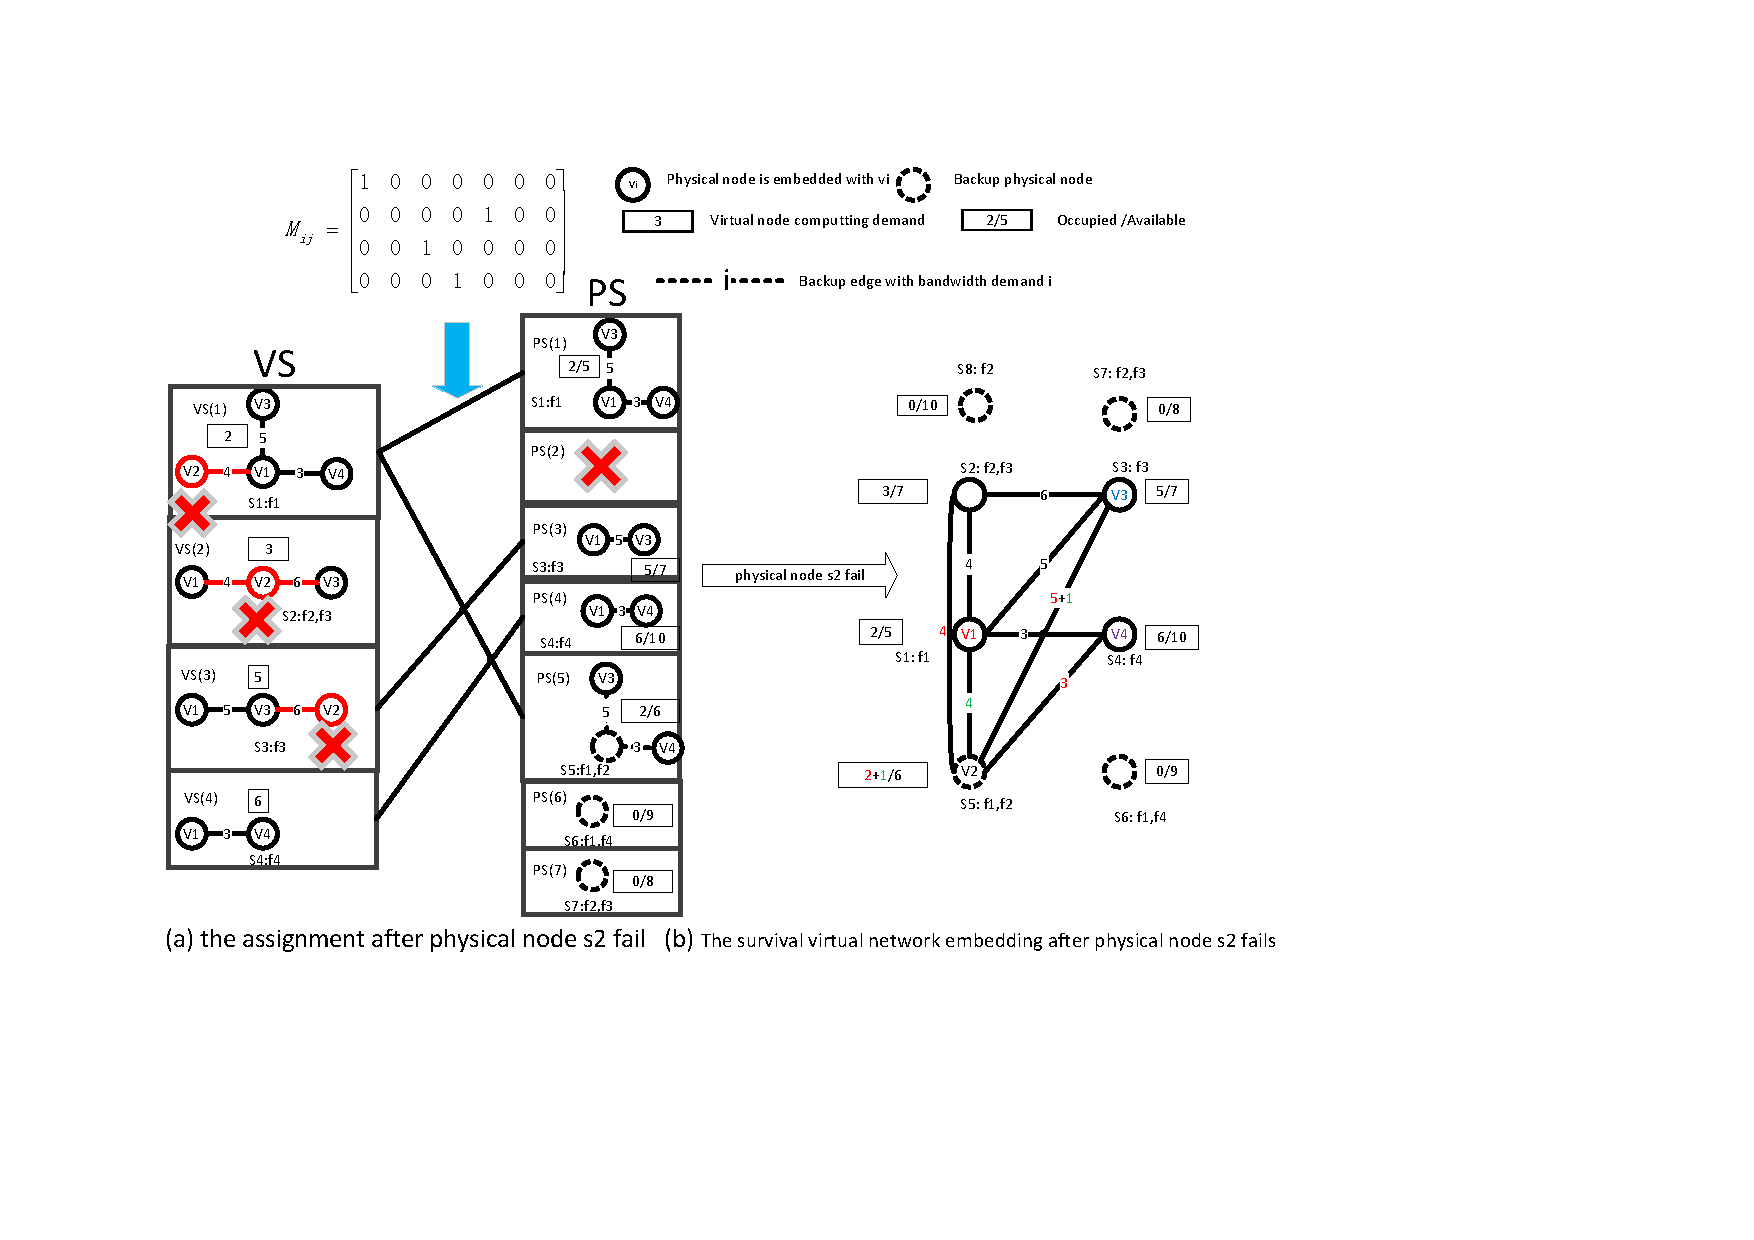
\includegraphics[width=4in]{Fig/Node2Failure}\\
  \caption{Node2Failure}\label{fig:Node2Failure}
\end{figure}

\begin{figure}
\centering
% Requires \usepackage{graphicx}
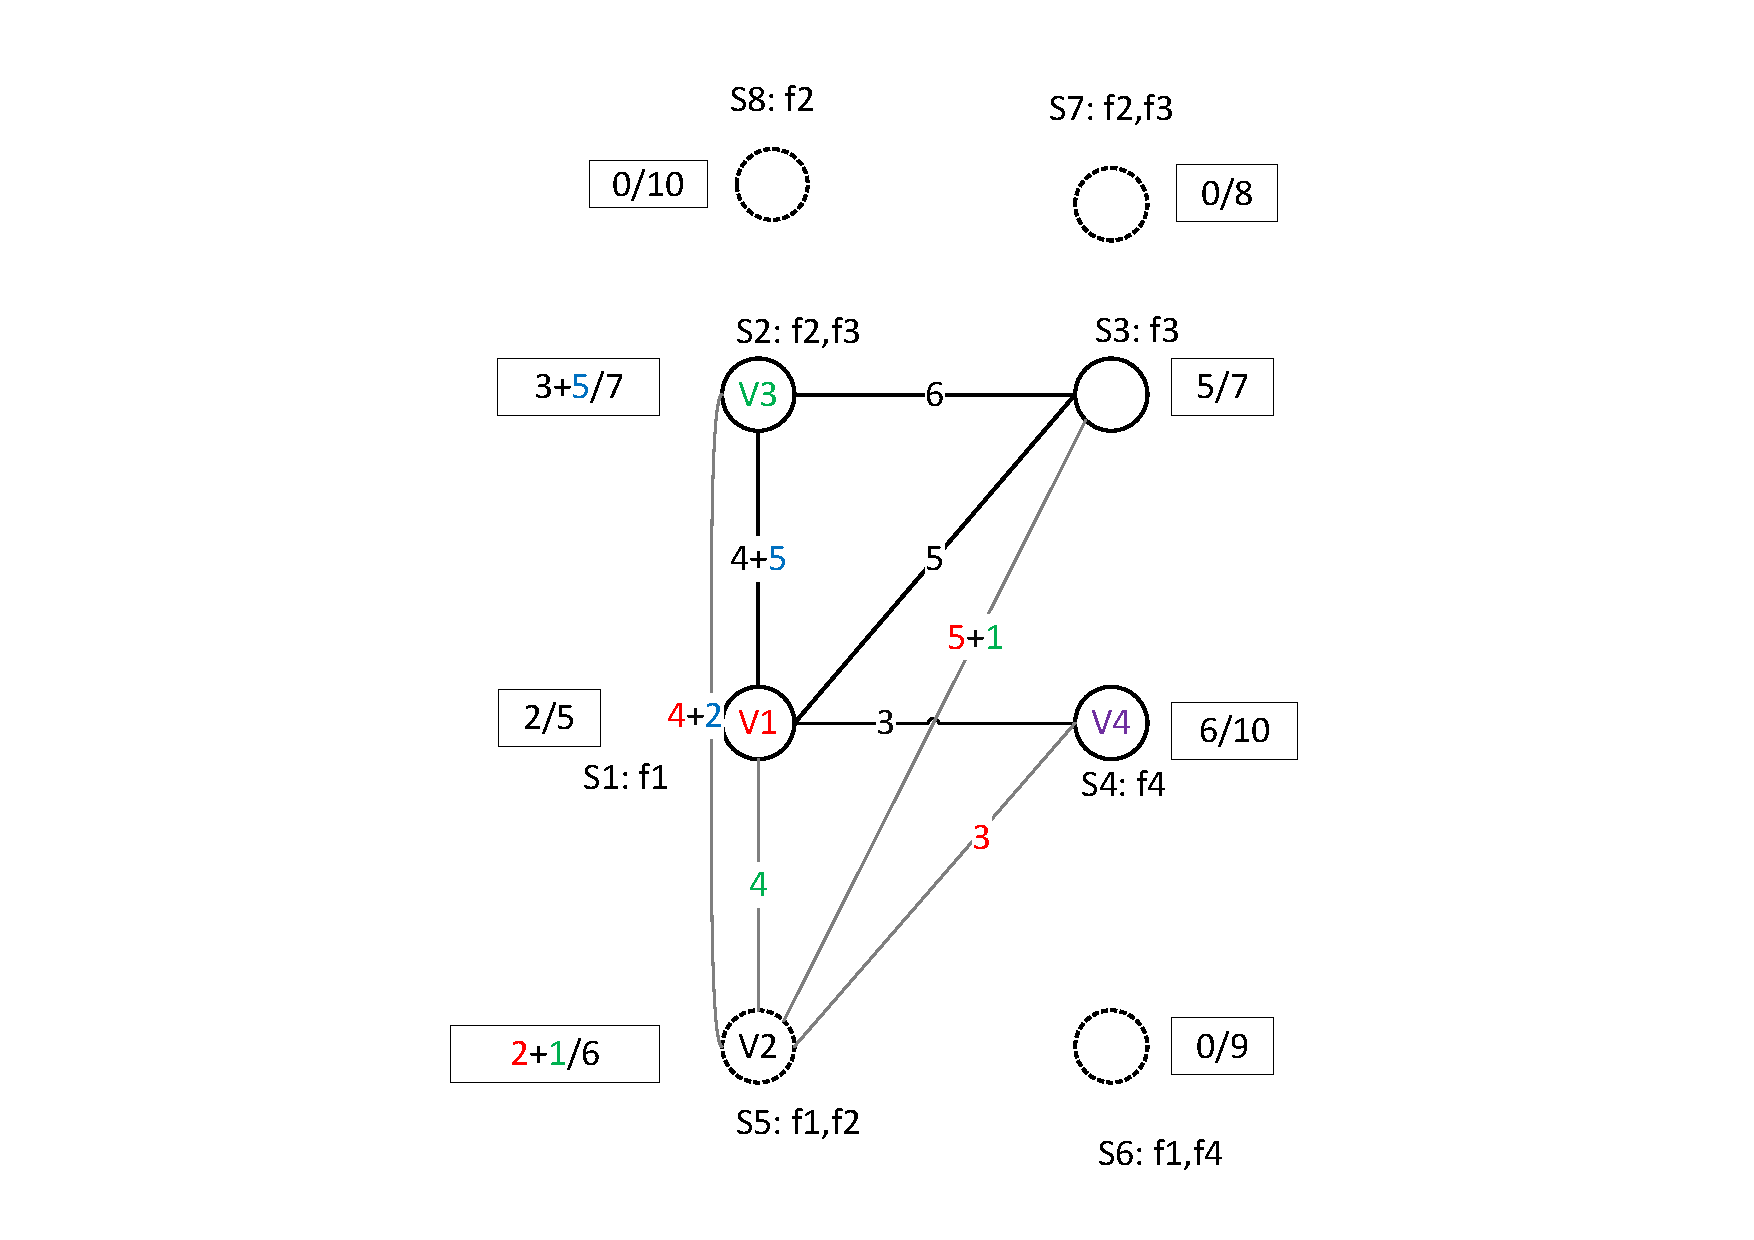
\includegraphics[width=2in]{Fig/Node3Failure}\\
  \caption{Node3Failure}\label{fig:Node3Failure}
\end{figure}

\begin{figure}
\centering
% Requires \usepackage{graphicx}
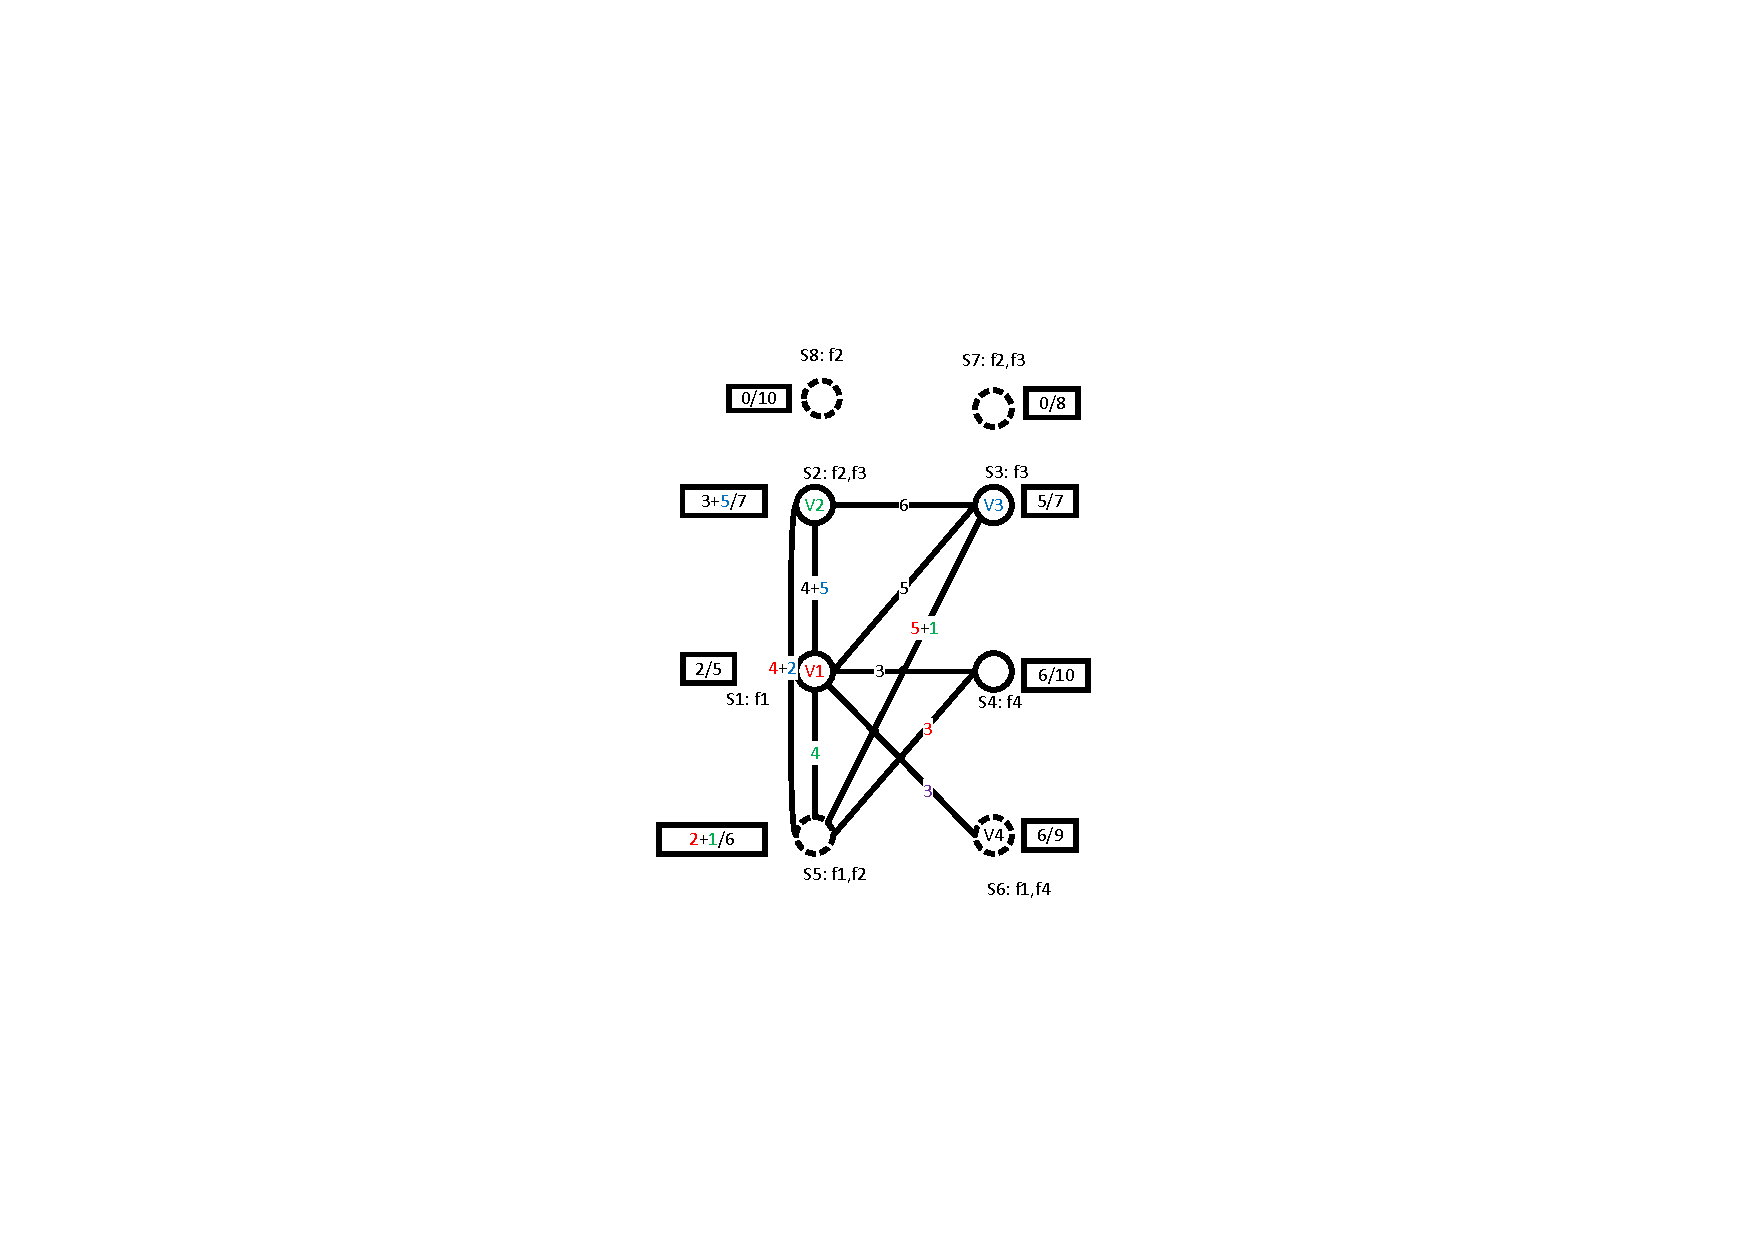
\includegraphics[width=2in]{Fig/Node4Failure}\\
  \caption{Node4Failure}\label{fig:Node4Failure}
\end{figure}











%
%it will be clear from the preceding examples that is is by no means easy to determine whether G is a subgraph of G*-v.
\section{requesting survival virtual network using integer linear programming}
\label{sec:SVN_ILP}
The one of contributions of this paper is the modelization of specific node fault tolerant problem as an optimization. The general technique used to solve this problem is a combined algorithm consisting of enumeration and Ullmann Algorithm\cite{ullmann1976algorithm}, which is proposed as a  algorithm of exponential complexity which is brute force method briefly. More precisely, we propose an Integer Linear Program(ILP)\cite{schrijver1998theory} model of this problem. In the following, We briefly explain how to solve a problem using ILP.

\subsection{Modeling the SNFT problem}
In this section, we formulate the problems discussed in the previous sections with Integer Linear Program(ILP) method. Though we have proved that these problems are NP-complete, as we will demonstrate later, the ILP formulation of the problem provides a very viable tool for solving it, for most real-world virtual network request which typically have less than a few hundred nodes and edges. Throughout this section, we will focus exclusively on the survival virtual network request [$G(V,E,S),B(V,S))$], we assume that $G$ is simple directed service label graph.
%the term graph represents a loop undirected non multidigraph. As a consequence, an edge e originating from i and targeting to j and can be denoted ij without any ambiguity.

%In order to model the problem as an ILP, we use binary variables, i.e. C=$\{0,1\}^n$
%transform the graph for reduce the constrain condition of service function.\ref{fig:ILP_transfromed_graph},\ref{fig:ILP_inserted_augmented_transformed_graph}.

To begin with, we introduce some necessary notation:

$MBG$: $[mbg_{u,v}]_{(|V|+|B|)\times (|V|+|B|)}$, the adjacency matrix of graph $G^o$. where

${mbg_{u,v}}=\left\{ \begin{array}{l}
1\ if\ edge\ e\ originates\ from\ u\ to\ v\\
0\ otherwise
\end{array} \right.$ \\

$MAG$: $[mag_{u,v}]_{|V|\times |V|}$, the adjacency matrix of arbitrary graph $G$. Where

${mag_{u,v}}=\left\{ \begin{array}{l}
1\ if\ edge\ e\ originates\ from\ u\ to\ v\\
0\ otherwise
\end{array} \right.$ \\

%matrix of service functions set corresponding to node
$T^{l}$: $[t^l_{u,v}]_{|V|\times (|V|+|B|)}$, The $l$-th node permutation matrix against $l$-th node failed. Where

${t^l_{u,v}}=\left\{ \begin{array}{l}1\ if\ node\ u\ transformed\ to\ node\ v\\
0\ otherwise
\end{array} \right.$.

$MBS$: $[mbs_{u,v}]_{(|V|+|B|)\times |S|}$, incidence matrix of specific services of the SNFT graph $G^o$. where

${mbs_{u,v}}=\left\{ \begin{array}{l}1\ if\ node\ u\ have\ specific\ flag\ v\\
0\ otherwise
\end{array} \right.$.

$MAS$: $[mas_{u,v}]_{|V|\times |S|}$, incidence matrix of  specific services of the arbitrary graph $G$. where

${mas_{u,v}}=\left\{ \begin{array}{l}1\ if\ node\ u\ have\ specific\ flag\ v\\
0\ otherwise
\end{array} \right.$.

$AugB$:$[aug_i]_{|B|}$, whether the i-th backup nodes is used or not. where

${aug_i}=\left\{ \begin{array}{l}1\ if\ node\ i\ is\ used\\
0\ otherwise
\end{array} \right.$.

The problem of requesting 1-specific node fault tolerant graph [$G(V,E,S),B(V,S))$] can be formulated as the folowing ILP problem:
\begin{center}
\begin{align}
\label{equ:ILPC1}such\ as:\ T^l*(T^l* MBG)^{'}&\geq MAG\\
\label{equ:ILPC2} \sum_{1\leq v\leq (n+b)}T^l_{iv}&= 1 (1\leq i\leq n)\\
\sum_{1\leq u\leq n}T^l_{uj}&\leq 1 (1\leq j\leq (n+b)) \notag \\
\sum_{1\leq u\leq n,1\leq v\leq (n+b)}T^l_{uv}&=n \notag\\
\label{equ:ILPC5}  T^k_{uk}&=0 (1\leq u\leq n)\\
\label{equ:ILPC7} MAG_{uv}&\leq MBG_{uv}(1\leq u\leq n,1\leq v\leq n)\\
\label{equ:ILPC8} MAS&\leq T^l*MBS\\
\label{equ:ILPC9} \frac{\sum_{1\leq v\leq (n+b)}MBG_{(n+i)v}+n-1}{n} &\leq B_i(1\leq i\leq b)\\
\end{align}

\end{center}

\begin{itemize}
\item Constraint(\ref{equ:ILPC1}) guarantees that when the l-th critical node of graph $G$ failed, we could find subgraph which is subgraph isomorphism of SNFT graph $G^o$. we represent the mapping relation as permutation matrix in view of Ullman\cite{ullmann1976algorithm}
\item Constraint(\ref{equ:ILPC5}) implies that operation of the transform matrix of mapping relation is appropriate and correct format in respect with one node failure.
\item Constraint(\ref{equ:ILPC7}) guarantees that SNFT graph $G^o$ must be the augmented graph of previous graph $G$.
\item Constraint(\ref{equ:ILPC8}) guarantees that when the l-th node failed  all nodes of the transformed graph still have specific flag, which is specific flag of corresponding node of previous graph $G$.

\end{itemize}
%
%\begin{figure}
%\centering
%% Requires \usepackage{graphicx}
%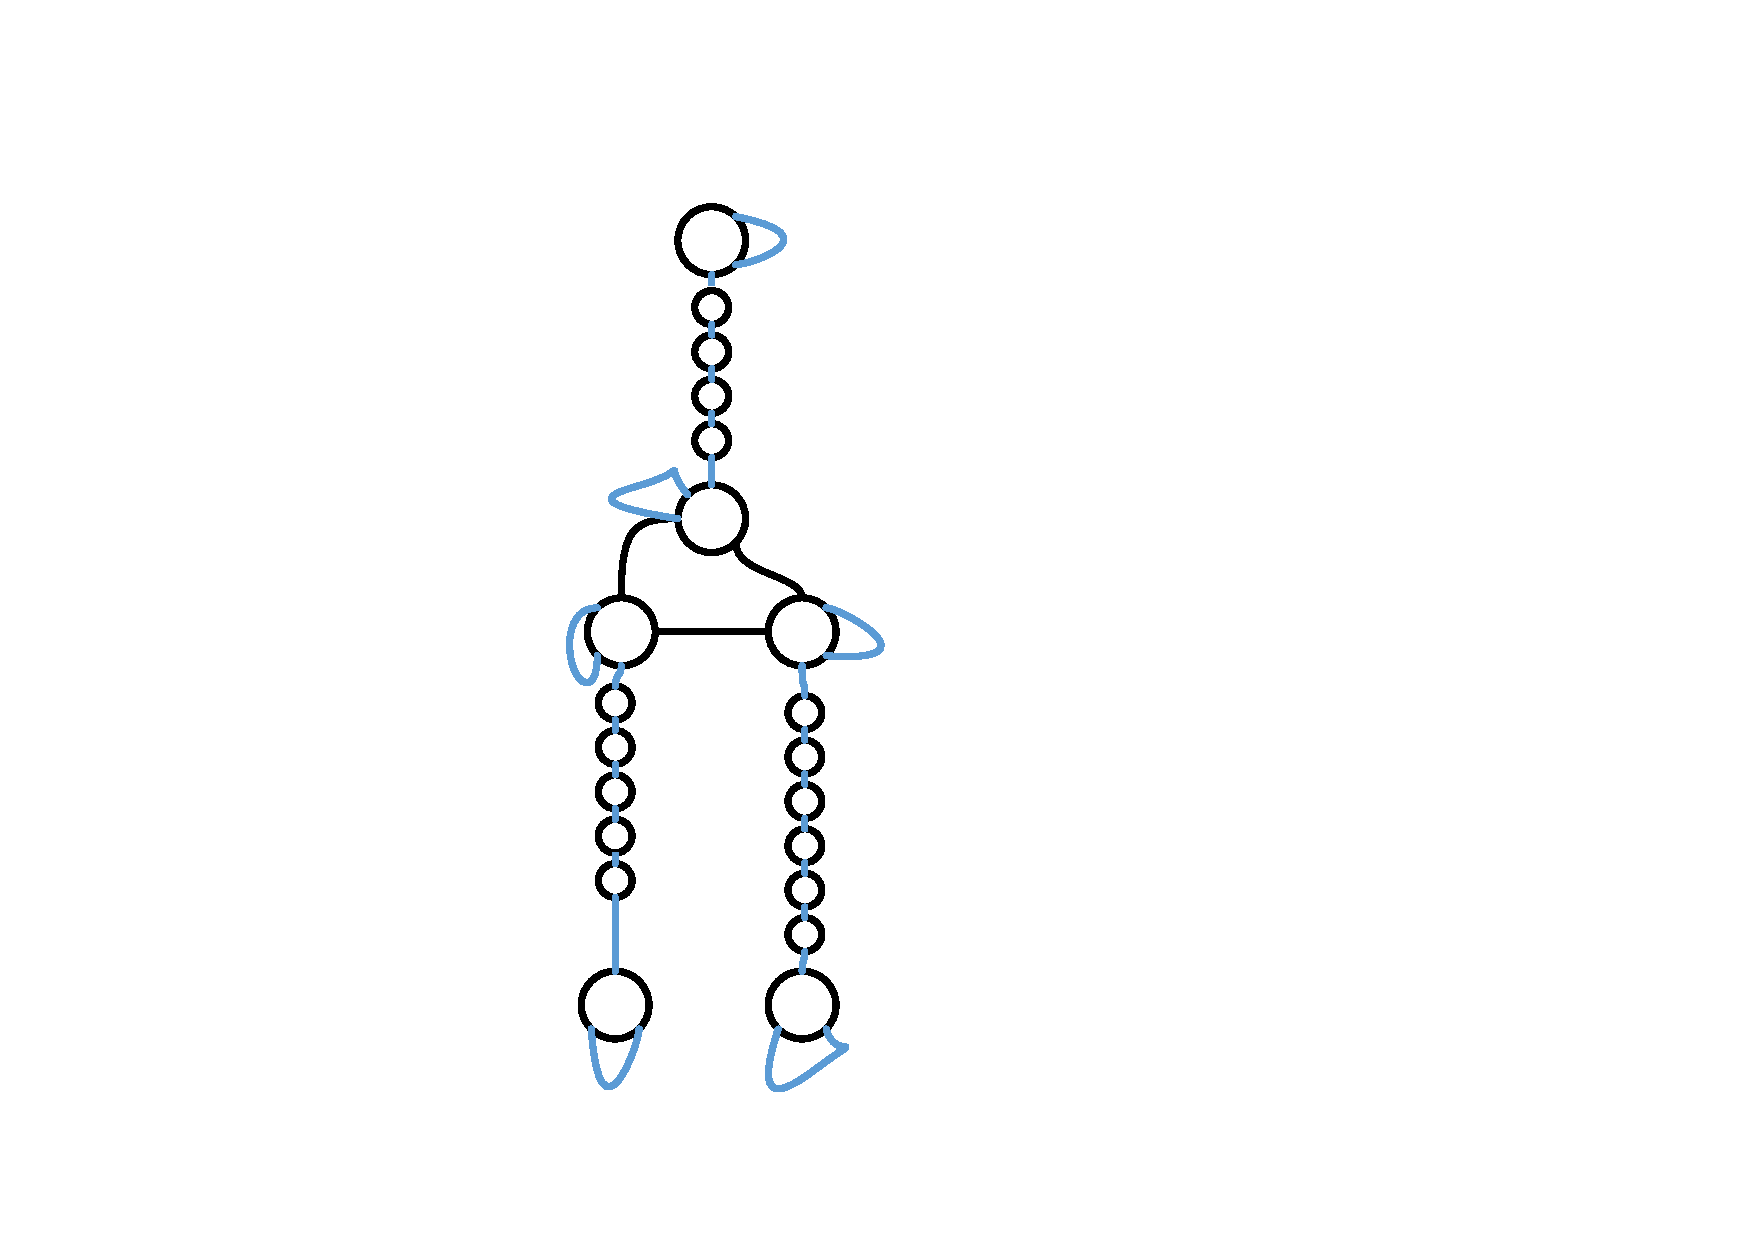
\includegraphics[width=2.5in]{ILP_transfromed_graph}\\
%\caption{transformed Graph G}\label{fig:ILP_transfromed_graph}
%\end{figure}
%
%\begin{figure}
%\centering
%% Requires \usepackage{graphicx}
%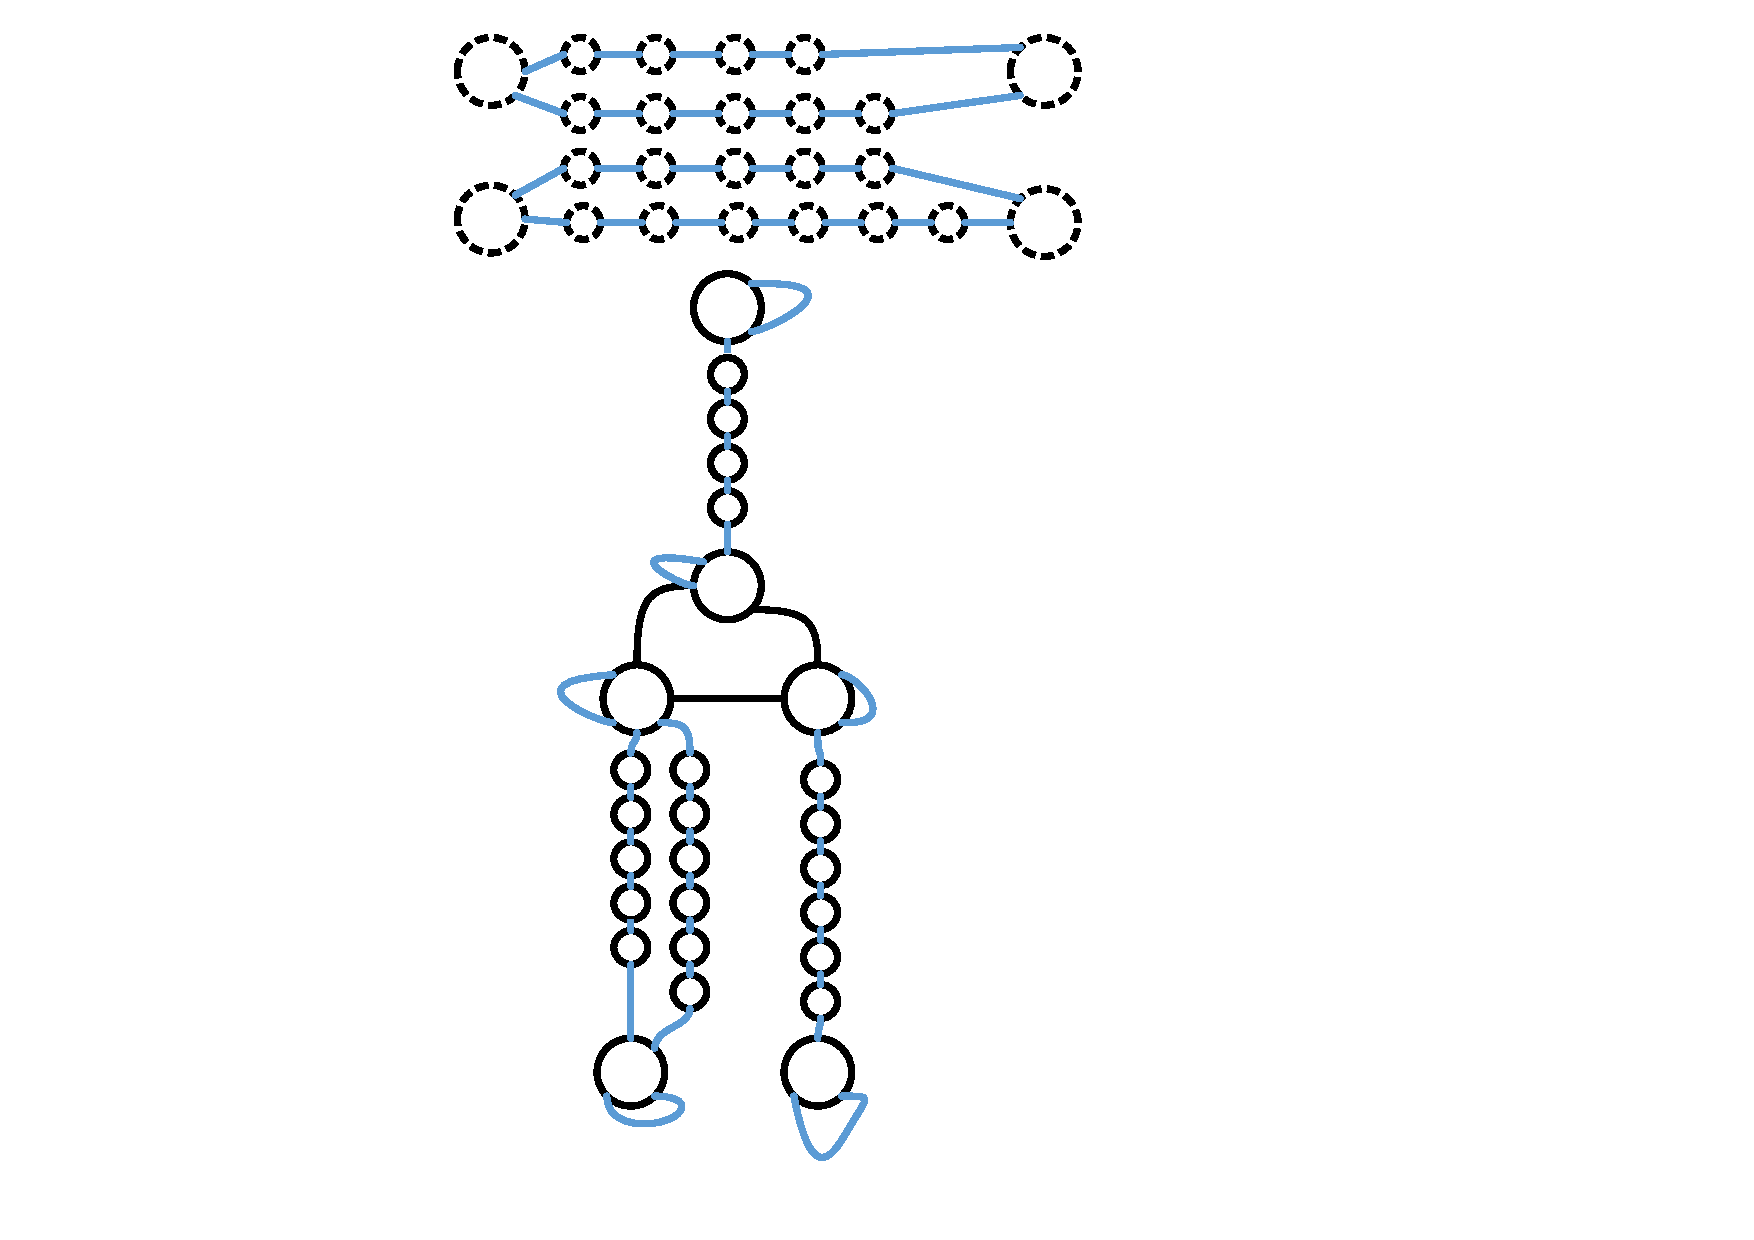
\includegraphics[width=2.5in]{ILP_inserted_augmented_transformed_graph}\\
%\caption{transformed Graph of to be augmented graph G}\label{fig:ILP_inserted_augmented_transformed_graph}
%\end{figure}

\subsection{Objective Function and Approximation}
We seek to minimize the amount of resource used for a VInf. The object function of the adapted ILP is then
\begin{align}
min: \alpha \sum_{1\leq i\leq b}B_i+ & \notag \\
\beta \times(\sum_{1\leq u\leq (n+b) 1\leq v\leq (n+b)}MBG_{uv}-&\sum_{1\leq u\leq n,1\leq v\leq n}MAG_{uv})
\end{align}
where $\alpha$ and $\beta$ are node and link weights, respectively. To achieve minimize the amount of nodes, the weight can be set as $(n^2+1)$ and $1$, respectively.

The presence of the boolean variables turns the linear program into a NP-Hard problem. An alterative is to relax the boolean variables to real-value variables, obtain an approximate virtual node transformation.




\begin{equation}
dp[i][{W_1}][{W_2}] \ldots [{W_m}] = \left\{ \begin{array}{l}
dp[i - 1][{W_1} - {w_i}][{W_2}] \ldots [{W_m}] + {v_i}\\
dp[i - 1][W][{W_2}_{} - {w_i}] \ldots [{W_m}] + {v_i}\\
dp[i - 1][W][{W_2}_{}] \ldots [{W_m} - {w_i}] + {v_i}
\end{array} \right\}
\end{equation}

$n*\prod_{i=1}^mC_i$

$m*n*\prod_{i=1}^mC_i$

\section{Heuristics Algorithms}
\subsection{Heuristics Algorithms Design Formulation of SeVN }
\label{sub:SeVNDesignFormulation}
With the discussion above, for a given N-nodes VNR, SeVN is designed within augment graph $G^*$ of N+k nodes through properly selecting the necessary nodes or links between these nodes and dimensioning the resources requirements associated with these nodes and links.

Our design objective is to minimize the total amount of such resources(startup node number, node computing, edge bandwidth) while still guaranteeing that if a node fails (that is, the node and its adjacent links are removed in the graph $G^*$) virtual network request's topological graph still keep integration of graph $G$ topological structure and insist normal work, we can still assign each node/link of VN to a node/link of the SeVN, that has sufficient node computing and edge's bandwidth resources respectively. It is our objection that firstly minimize number of start-up backup nodes, then minimize node computing resource, last minimize edge bandwidth resource to construct function node fault tolerant graph $G^*$.

Furthermore, there are two different cases. If re-embedding or migrating the unaffected node(un-failed node) is allowed for failure recovering, it is known as the FD-SeVN design problem. Otherwise, after each failure, if the failed node is restored in the only one backup node without migrating other unaffected node, it is referred to as the FI-SeVN design problem. Generally speaking, designing FD-SeVN is a combinatorial optimization problem and needs to be investigated in depth, while FI-SeVN exists exclusively and could be figured out easily.


\subsection{Design Procedure}

%这样转可以还原的。为什么。
In this section, we propose a heuristic algorithms for FD-SeVN problem, as well as an SeVN problem's algorithm with resources sharing consideration fitting for both FD-SeVN and FI-SeVN.

Decompose topological graph of  virtual network $VN$ into N star structure $STAR$, construct match relationship between star structures. This match relationship is corresponding node transform cost relationship.

However, as a matter of fact, computing the minimum additional resources needed to convert one attributed graph to another (hereafter called graph alignment problem, GAP) is an NP-complete problem which could be reduced from the Graph Edit Distance problem \cite{justice2006binary}. Therefore, we propose a heuristic algorithms in detail, and we first decompose a graph to a set which contains star structures which retains certain structural information of the graph of embedded virtual network. Then, the graph alignment cost could be approximated by the matching cost(transform cost) between two graphs based on their star representations. This approach is elaborated as follows.


The general idea of the heuristic for FD-SeVN design is to consider the failure of primary nodes in virtual network node's label sequentially, and in each step, compute the minimum additional resources needed to reassign the task graph based on an incremental approach (i.e., recovering from the current node failure should take not only the survived primary nodes/links resources into consideration, but also the survived redundant resources reserved for previous node failure). After iteratively execute all the node failures, SeVN is constructed within the Star Structure with the added redundant resources in each step. Generally speaking, select a optimal node $v_i$ to minimum additional resource with respect to every steps.(Min value for every step )


%This translates to ensuring that every backup node has guaranteed bandwidth to all neighbors of all critical nodes.

Redistribute physical resource corresponding to augment graph $G^i$  with additional computational and bandwidth resource. concrete step is that apply for computational resource for virtual nodes and complete path around bandwidth for virtual edges.


%At the same time, for the task graph reassigning approach in
%Edit Grid, we also introduce the permutation matrices, which is
%an (N+1)×(N+1) orthogonal matrix having PPT = PT P = I
%(where I is the identity matrices), to indicate the corresponding
%state vector transformation of Edit Grid. Assume at this point
%that the initial state of the Edit Grid η0 contains the given task
%graph in its standard placement. And we have another state η1
%such that it describes task graph situated on the Edit Grid in a
%different way as shown in Fig. 3(c), as well as its state vector
%shown in Table I. Based on the knowledge in graph theory,
%the two graphs corresponding to these different states of Edit
%Grid are isomorphic [14] which suggests that there is a bijection
%between these two attributed graphs. So, we could employ
%permutation matrices to implement task graph reassignment in
%Edit Grid. For example, with the following Edit Grid state η0 :


\subsection{FD-SeVN Algorithm}
\subsubsection{Graph Decomposition}
Star Structure: A star structure s is an attributed, single-level, rooted tree which can be represented by a 7-tuple $star=(v^*,c^*,C^*,f^*,F^*,L^*,B^*)$ as shown in Figure \ref{fig:StarRepresentation}, where $v^*$ is the root node, $c^*$ is the  node's demand computing, $C^*$ is the node's remain computing capacity could be resigned again, $f^*$ is the node's function type, $F^*$ is function type set of the node, $L^*$ is other all nodes  adjacent with nodes $v^*$, $B^*$ is the bandwidth of each link $e_{ij}$ associated with the root node $v^*$. Edges exist between the root node and its adjacent nodes, and no edge exists among its adjacent nodes.

More exactly, for node $v_i$ in an attributed graph  $G^V (V^V,E^V,f^V,F^V,L^V,C^V,B^V,M^V)$, we can generate a star structure $star_i$ corresponding to $v_i$ in the following way, $star_i=(v^V_i,c^V_i,C^V_i,f^V_i,F^V_i,L^V_i,B^V_i)$ where $f^V_i$ is a function type $f_i$ running in node $v_i$, $F^V_i=\{f_{j}|$ for all $f_j$ belong node $v_i$ function set$\}$.  $L^V_i=\{v_j|$ for all nodes $v_j$  adjacent with node $v_i\}$, $B^V_i=\{b_{i,j}| $ for all $e_{i,j}\in L^V_i\}$. Accordingly, we can derive $N$ star structures from topological graph of substrate network with embedded virtual network of N nodes (we uniformly discuss all N virtual nodes fail). In this way, topological graph of embedded virtual network can be transformed to a  star structure. A quintesfntial example should be cited that construct $star_2$ corresponding to node $v_2$, $star_2=(v_2,3,7,f_2,\{f_2,f_3\},\{v_1,v_3\},\{b_{21}=4,b_{23}=6\})$, virtual node $v_1$ correspond star structure $star_1=(v_1,2,5,f_1,\{f_1\},(v_2,v_3,v_4),\{b_{12}=4,b_{13}=5,b_{14}=3\})$.
%, $C^*$ is the computation resource requirement of every nodes, $C^n=\{C^n_{u}|$for all $e_{n,u}\in E\}$
%\begin{figure}
%\centering
%% Requires \usepackage{graphicx}
%\includegraphics[width=3in]{fig/GraphDecomposition}\\
%\caption{Graph Decomposition}\label{fig:GraphDecomposition}
%\end{figure}

\subsubsection{Match Items}
Based on the topological graph of the embedded virtual network, we construct star structure set $STAR^L$, which erase some star structure corresponding to one substrate node without embedding virtual node. when calculating the virtual node $v_i$ which map to substrate node $s_i$ failure, constructing star structure set $STAR^R$ with erasing the node $v_i$ and the edge adjacent with node $v_i$ as shown in Fig.\ref{fig:StarRepresentation}.
\begin{figure}
\centering
% Requires \usepackage{graphicx}
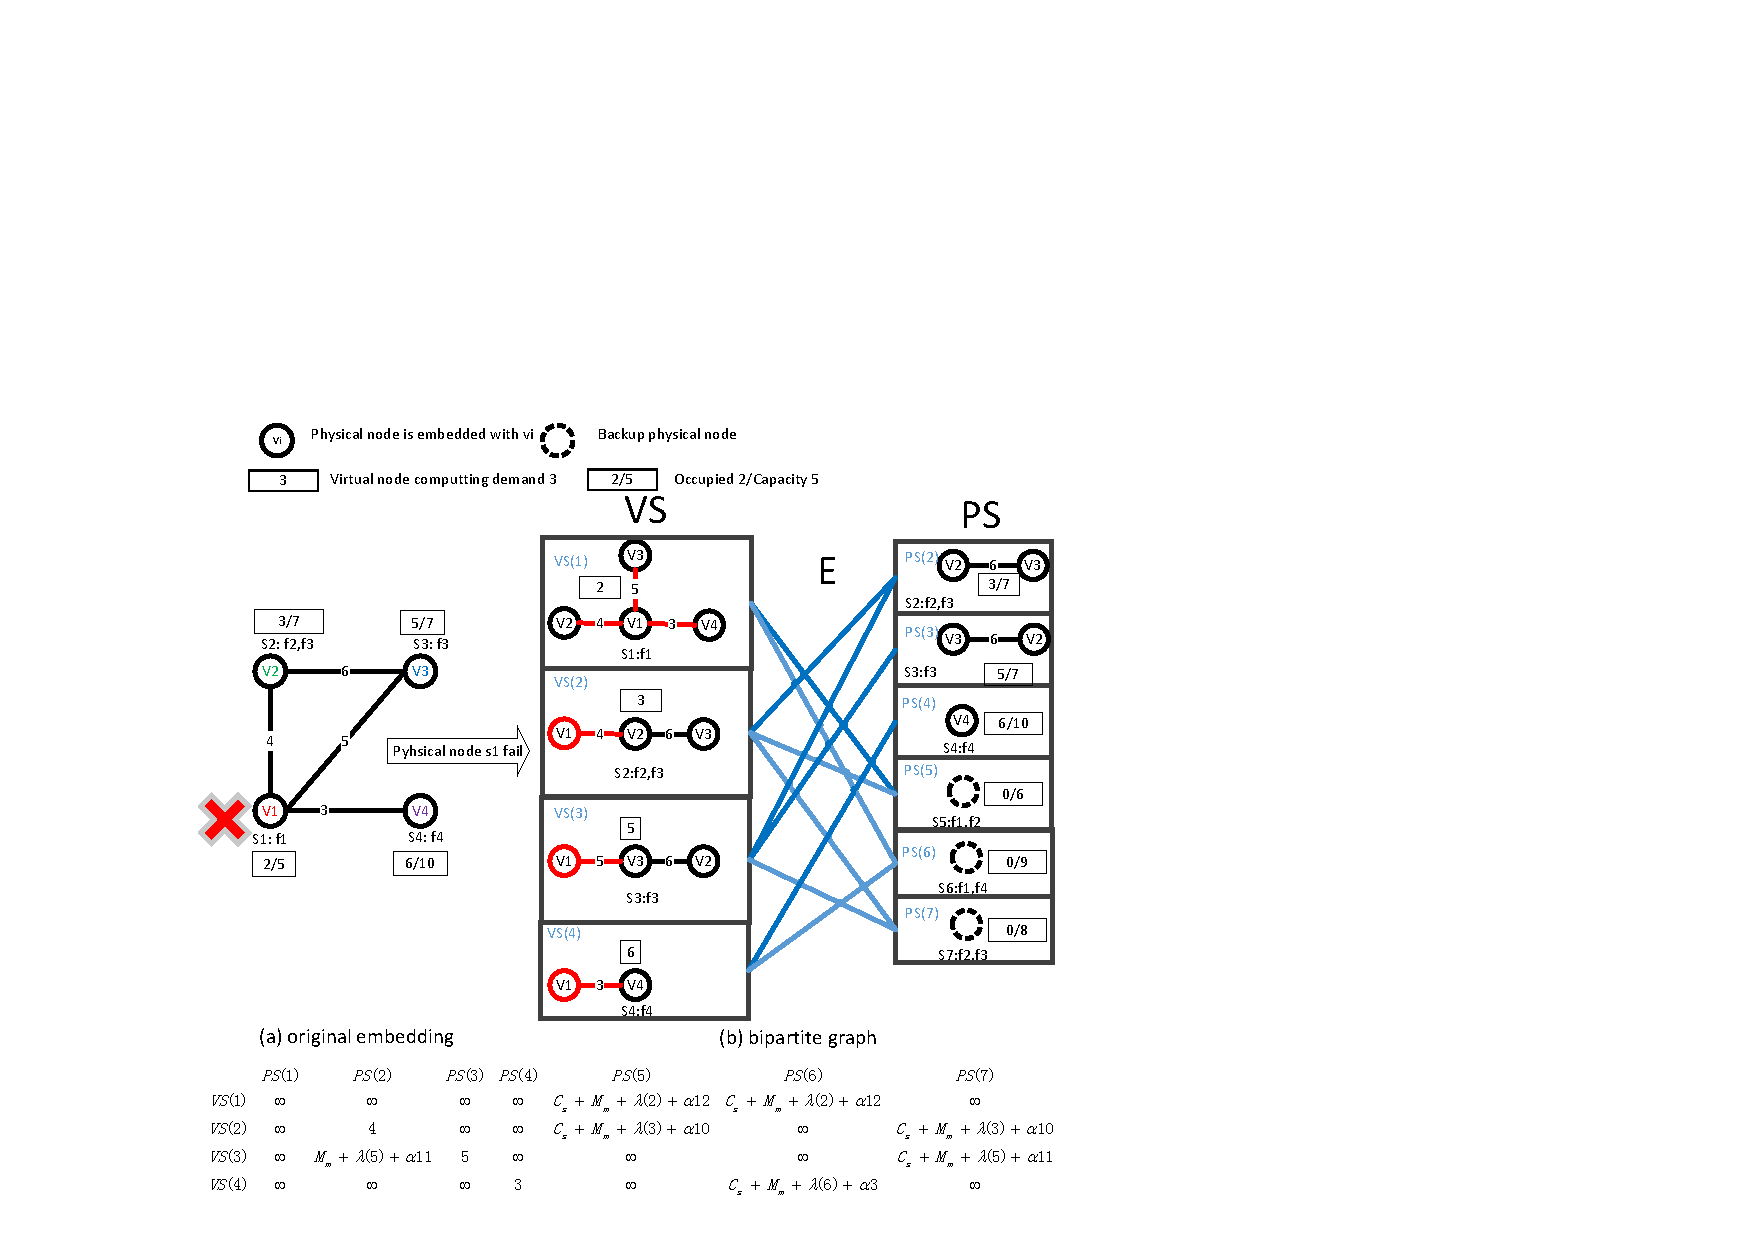
\includegraphics[width=3in]{Fig/StarRepresentation}\\
  \caption{The star representation of the embedded virtual network ($STAR^L$) and residual task graph after failure of node $v_1$ ($STAR^R$);}\label{fig:StarRepresentation}
\end{figure}
\subsubsection{Alignment Cost Matrix}
Due to the particularity of star structure, the alignment cost between two star structure set can be computed easily as below. For the two star structures $star^L_i$ and $star^R_j$ which is from $STAR^L$ and $STAR^R$ respectively, if node $f_i^V$ of $star^L_i$  is not included in $F^V_j$, the alignment cost of $star^L_i$ to $star^R_j$ is $\infty$, otherwise the alignment cost of $star^L_i$ to $star^R_j$ is
%equation \ref{equ:alignmentcost}:
%\begin{equation}\label{equ:alignmentcost}
\[\lambda(star^L_i,star^R_j)=\sum\limits_{v_u\in L_i \cap L_j}\gamma|b_{i,u}-b_{j,u}|_0+\newline
\sum\limits_{v_u\in L_i - L_j}\gamma b_{i,u}+\beta|c_i-c_j|_0+ \delta(v_i,v_j)+\theta(v_j)\]
%\end{equation}
where $\delta$, $\theta$ and $|x|_0$ is defined as follows:

$\delta ({v_i},{v_j}) = \left\{ \begin{array}{l}
{\rm{M_{m}}}\\
0
\end{array} \right.\begin{array}{*{20}{c}}
v_i\neq v_j\\
{otherwise}
\end{array}$

$\theta ({v_j}) = \left\{ \begin{array}{l}
{\rm{C_{s}}}\\
0
\end{array} \right.\begin{array}{*{20}{c}}
v_j\ is\ free\\
{otherwise}
\end{array}$

$|x|_0 = \left\{ \begin{array}{l}
{x}\\
0
\end{array} \right.\begin{array}{*{20}{c}}
if\ x\geq 0\\
{if\ x\leq 0}
\end{array}$

$\delta(v_i,v_j)\neq 0$ indicates that  root node $v_i$ should be reallocated to node $v_j$. $M_m$ is migration cost, $C_s$ is startup new node cost.we define $\lambda(star_i,star_j)$ according to graph edit distance\cite{sanfeliu1983distance}. In mathematics and computer science, graph edit distance (GED) is a measure of similarity (or dissimilarity) between two graphs.

In this way, both the topological graph of  embedded virtual network and the residual graph are composed to two star structure sets. With such a graph decomposition once a specific virtual node failure, an alignment matrix of the two star structure set could be constructed based on the alignment cost definition above. Therefore, the proposed GAP could be transformed to a (multiple knapsack problem) which will be investigated in the following part. For example, the alignment cost matrix when virtual network $v_1$ fail as follow.
\begin{equation*}
\tiny{
 {\begin{array}{*{20}{c}}
&R_{S_{2}}&R_{S_3}&R_{S_4}&R_{S_5}&R_{S_6}&R_{S_{7}}\\
{L_{V_1}}&\infty&\infty&\infty&\fbox{$C_{s}$+(2)+12}&C_{s}+(2)+12&\infty\\
L_{V_2}&\fbox{4}&\infty&\infty&C_{s}+(3)+10&\infty&C_{s}+(3)+10\\
L_{V_3}&M_{m}+(5)+11&\fbox{5}&\infty&\infty&\infty&C_{s}+(5)+11\\
L_{V_4}&\infty&\infty&\fbox{3}&\infty&C_{s}+(6)+3&\infty\\
\end{array}}
}
\label{lab:Node1FaliureAlignmentMatrix}
\end{equation*}

To elaborate this approach, Figure \ref{fig:StarRepresentation} shows how the 4-nodes VN be decomposed into a set of four star structures (shown as $STAR_L$ ), and each containing a primary task node (also called root node which is highlighted and color as blue), its adjacent links and its neighboring nodes.

\subsection{Multiple Knapsack Problem}
Based on the discussion above, the computation problem of minimal graph alignment cost is transformed to solving optimal multiple knapsack problem, which is one of the fundamental combinational optimization problems. In our case, there are two sets of vertices corresponding to the two sets of star structure of $STAR_L$ and $STAR_R$ respectively, and the weight of the edge between star structures of $STAR_L$ and $STAR_R$ is the alignment cost between the corresponding two stars.

Firstly, we proposed the formalization of the multiple knapsack problem as follow:

$M_{ij}=1(1\leq i\leq n,1 \leq j \leq m)$ represent that whether the i-th virtual node map the j-th substrate node, n and m denote virtual node's size and substrate node's size respectively.

$Cost_{ij}(1\leq i\leq n,1 \leq j \leq m)$ represent that the cost of i-th virtual node map the j-th substrate node. $\infty$ represent that there is not map relationship.

$c_i(1\leq i\leq n)$ represent that the i-th virtual node demand computational resource, $C_i(1\leq i\leq m)$ represent that the i-th substrate network maximum useful computation resource.

Objection: minimum $Cost_{ij}*M_{ij}$

constraints: $\sum\limits_{1\leq j\leq m} M_{ij}=1$,$\sum\limits_{1\leq i\leq n} c_i*M_{ij}\leq C_j$

\subsubsection{Dynamic Programming Equation}
\label{lab:DynamicProgrammingEquation}
We propose a dynamic programming equation method for solving the multiple knapsack problem. Assume $C_1,C_2,\ldots,C_n$, $C$ are strictly positive integers. Define $dp[i][{C_1}][{C_2}] \ldots [{C_m}]=0$ to be the minimum value that can be attained with n capacity variables  which less than or equal to $C_i$ using items up to knapsack i.

Initial state $dp[i][{C_1}][{C_2}] \ldots [{C_m}]=0$ is firstly assigned as infinity $\infty$. $dp[i][{C_1}][{C_2}] \ldots [{C_m}]=0$ when there is no any virtual node which is confirmed to map into another node. The total cost of current state is zero. $dp[i][{C_1}][{C_2}] \ldots [{C_m}]$ when  i nodes is succeeded to be mapped another nodes. The total cost of current state is minimal cost from optimal node location.

We can define $dp[i][{C_1}][{C_2}] \ldots [{C_m}]$ recursively as in Equation \ref{equ:statetransferequation}, when put i-th node into another node, in this situation, the current state is calculated from former i-1 nodes are succeeded to be mapped.

\begin{equation}
\label{equ:statetransferequation}
\min \left\{ \begin{array}{l}
dp[i - 1][{C_1-c_i}][{C_2}] \ldots [{C_m}]+\lambda(star^L_i,star^R_1)\\
dp[i - 1][{C_1}][{C_2-c_i}] \ldots [{C_m}]+\lambda(star^L_i,star^R_2)\\
...\\
dp[i - 1][{C_1}][{C_2}] \ldots [{C_m-c_i}]+\lambda(star^L_i,star^R_n)
\end{array} \right.
\end{equation}

dynamic programming method  could be applied to solve the multiple knapsack problem whose time complexity is $O[(n+b)*n*\prod_{i=1}^{n+b}C^i]$, which is pseudo-polynomial time. Space complexity is $O[n*\prod_{i=1}^{n+b}C^i]$.









\section{SeVN augment resource embed formulation}
In this section, we refer that design procedure of augmented resource allocation  of SeVN graph, we also give out resource demand allocation method fitting for both FD-SeVN and FI-SeVN embedding, since the difference between FD-SeVN and FI-SeVN in embedding approach could be reconciled by a general resources sharing constraint. More details would be elaborated in the following part.

Besides, with respect to the node embedding even and virtual links embedding, because not all the virtual links or not all their bandwidth would be employed simultaneously under single node failure, some virtual links could share substrate resources if they are embedded on the same substrate link, which would reduce the total substrate bandwidth needed.


\subsection{Embed Augmented Backup Resource}
From Sec.\ref{lab:DynamicProgrammingEquation}, we have obtained map relationship with respect to node $v_i$ failure, then compute out that every node should to be reallocated how much computation and every link should to be reallocate how much bandwidth in substrate network SN as shown in Fig.\ref{fig:AugmentResource}. As most virtual network embedding algorithm, node mapping phase had been completed with respect to our algorithm, the next procedure give out edge mapping phase. we use standard shortest path algorithm, dijkstra algorithm, for requesting path of substrate node with respect to every virtual network's node, then reallocate some bandwidth to this path of substrate network for this virtual network survivable request.

\begin{figure}
  \centering
  % Requires \usepackage{graphicx}
  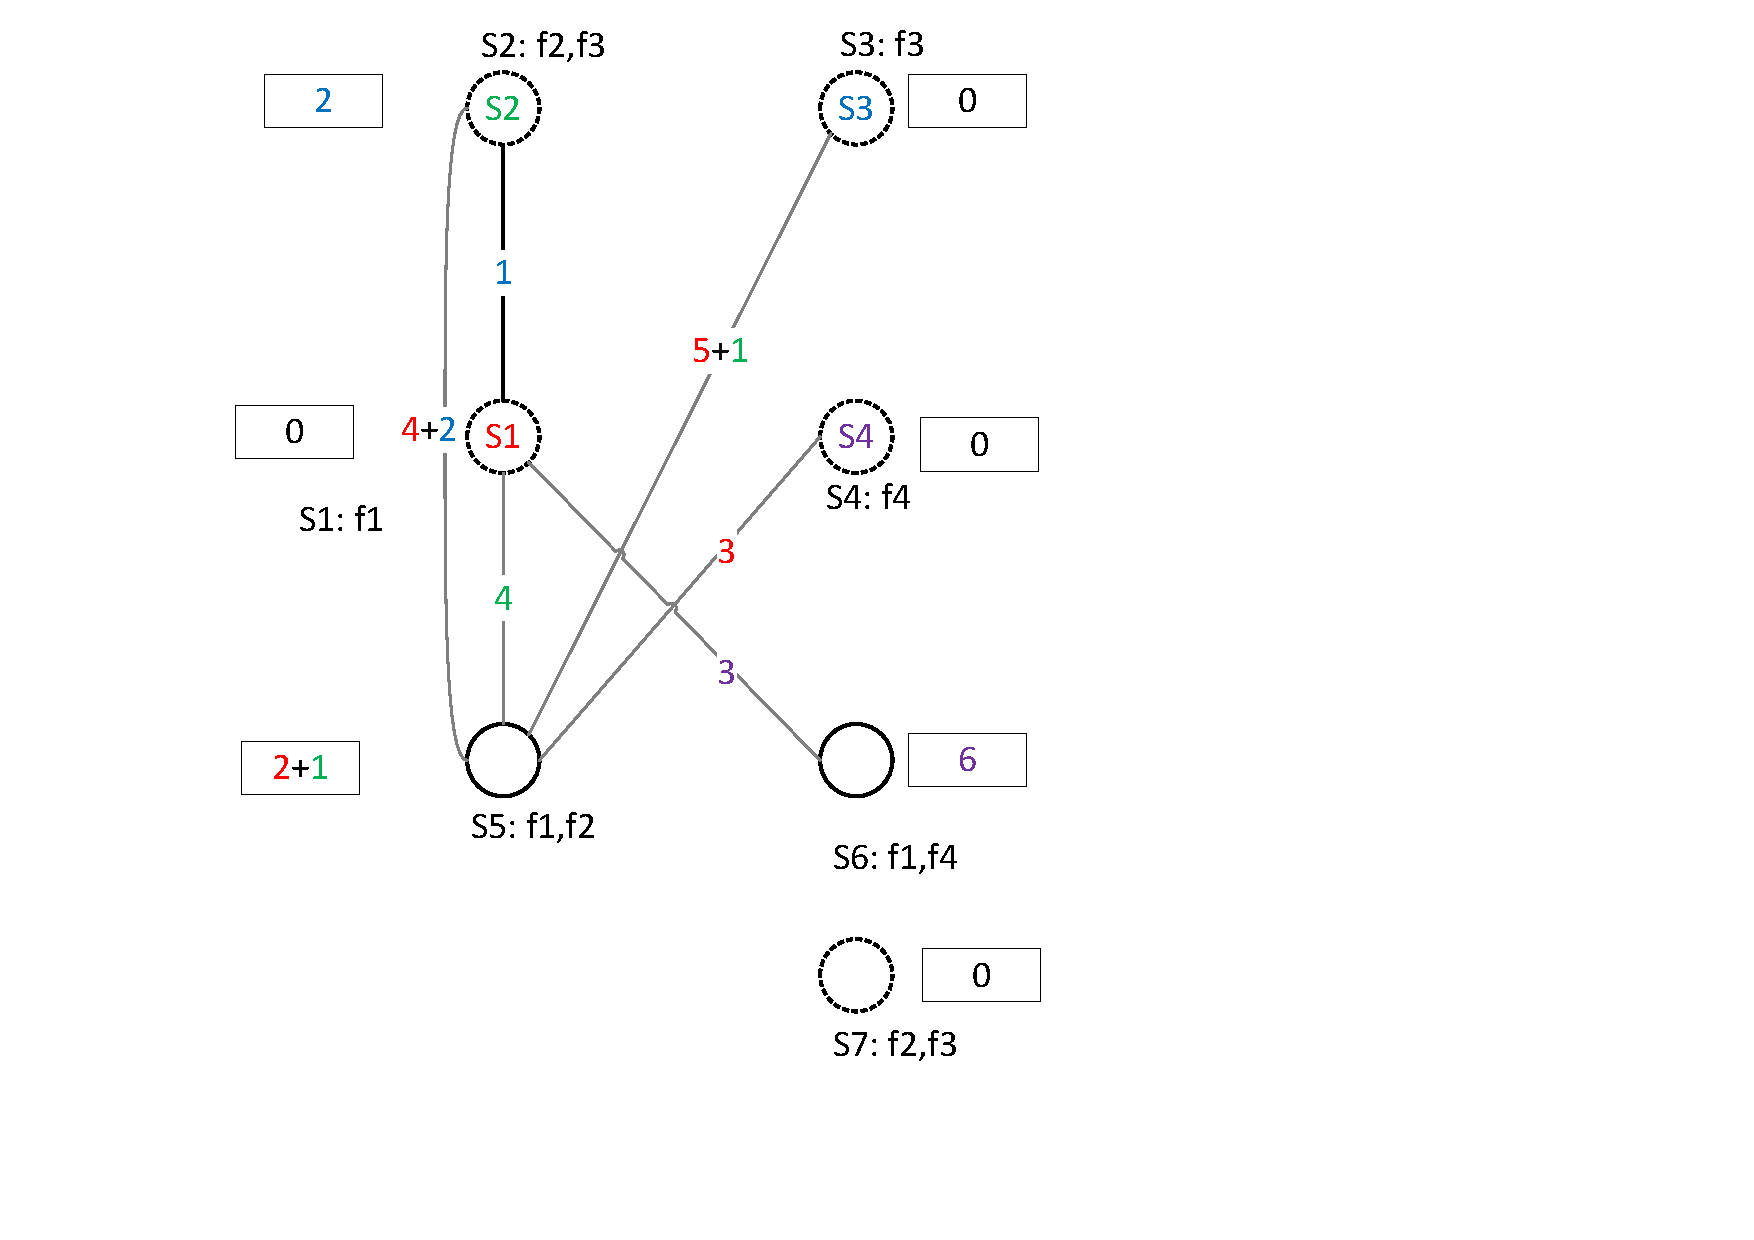
\includegraphics[width=2in]{Fig/AugmentResource}\\
  \caption{Augmented Resource}\label{fig:AugmentResource}
\end{figure}

Finally, we repeat the procedure of graph decomposition and multiple knapsack problem for each following node failure to construct the graph of final FD-SeVN. As shown in Fig.\ref{fig:FD}, partial augmented resource which is labeled consecutively with different color of the SeVN for each node failure is presented. It is worth noting that, every step of partial augmented resource is based on the previous step.

\subsection{Algorithm procedure}
In this section, we describe the whole our algorithm procedure of SeVN problem in Alg.\ref{lg:SeVNAlg}
\begin{algorithm}
\label{alg:SeVNAlg}
\caption{survivable embedded virtual network request algorithm}
\begin{algorithmic}[1]
\REQUIRE $G^V (V^V,E^V,f^V,C^V,B^V)$:  topological graph of virtual network's request; $G^S (V^S,E^S,F^S,C^S,B^S)$, topological graph of substrate network .
\ENSURE generate SeVN and embed SeVN augment resource into substrate network.
\STATE embed VN $G^V$ into substrate network $G^S$.
\STATE extract embedded virtual network eVN $G^*$ from SN corresponding to this VN embedding request
%\STATE AllMinimumCycle($G(V,E)$)
\FORALL{$v_i$ such that $v_i\in$ virtual node}
\STATE decompose eVN into two star structure sets $STAR^L$ and $STAR^R$ from graph $G^*$.
\STATE construct items based star structure set $STAR^L$.
\STATE construct knapsacks based star structure set $STAR^R$ from embedded virtual network eVN.
\STATE construct alignment cost matrix based graph edit distance method\cite{sanfeliu1983distance}
\STATE solve multiple knapsack problem through dynamic programming.
\STATE add new nodes ,connect new edge, allocate node computing and edge's bandwidth into $G^*$ to construct new graph $G^*$.
\ENDFOR
\STATE embed new additional(augment) boot up resource or startup new node from SeVN $G^*$ into substrate network $G^S$
\RETURN SeVN,$G^S$
\end{algorithmic}
\end{algorithm}

1 node+2 node computaion+12 bandwidth
0 node+1 node computaion+5 bandwidth
1 node+5 node computaion+11 bandwidth
1 node+6 node computaion+3 bandwidth
=3 node+14 node computaion+31 bandwidth

1 node+2 node computaion+12 bandwidth
0 node+1 node computaion+5 bandwidth
0 node+2 node computaion+3 bandwidth
1 node+6 node computaion+3 bandwidth
=2 node+11 node computaion+23 bandwidth


\subsection{Time Complexity}
The formulation of SeVN request problem indicates that this problem is a binary quadratically programming problem in optimization field , and the essence of SeVN problem solution is a series of permutation matrix  which determine the migration reassigning approach after each node failure. There are all $|V|$ nodes of virtual network failed, the time complexity of iteration in every nodes is $O[|V|*|S|*\prod_{i=1}^{|S|}c^i]$. Thus, its overall computation complexity is $O[|V|*|S|*|V|*\prod_{i=1}^{|S|}c^i]$, where $|V|$ is number of failure node.

\subsection{Subgraph Isomorphism Proof}
\label{sec:SubgraphIsomorphismProof}


Suppose certain one graph $G^o$ is subgraph of $G^*$. Based the mapping relationship from Sec.\ref{sub:SeVNDesignFormulation}, there must be a bijection mapping between node of graph $G$ and graph $G^o$. The some node $v_i$ of graph $G$ if and only if map a node $v_i^o$ of graph $G^o$. According to schema of our heuristic algorithm, there must exist one edge or create one edge ($v^o_iv^o_j$) regardless of  there is not edge between node $v^o_i$ and node $v^o_j$ , which is corresponding to edge $v_iv_j$ of graph $G$. Consequently, there must be a bijection function of every edge $e$ of graph $G$ to edge $e^o$ of graph $G^o$, $G$ is isomorphic to graph $G^o$, graph $G^o$ is subgraph of $G^*$, $G$ is subgraph isomorphism of graph $G^*$





\begin{figure}
  \centering
  % Requires \usepackage{graphicx}
  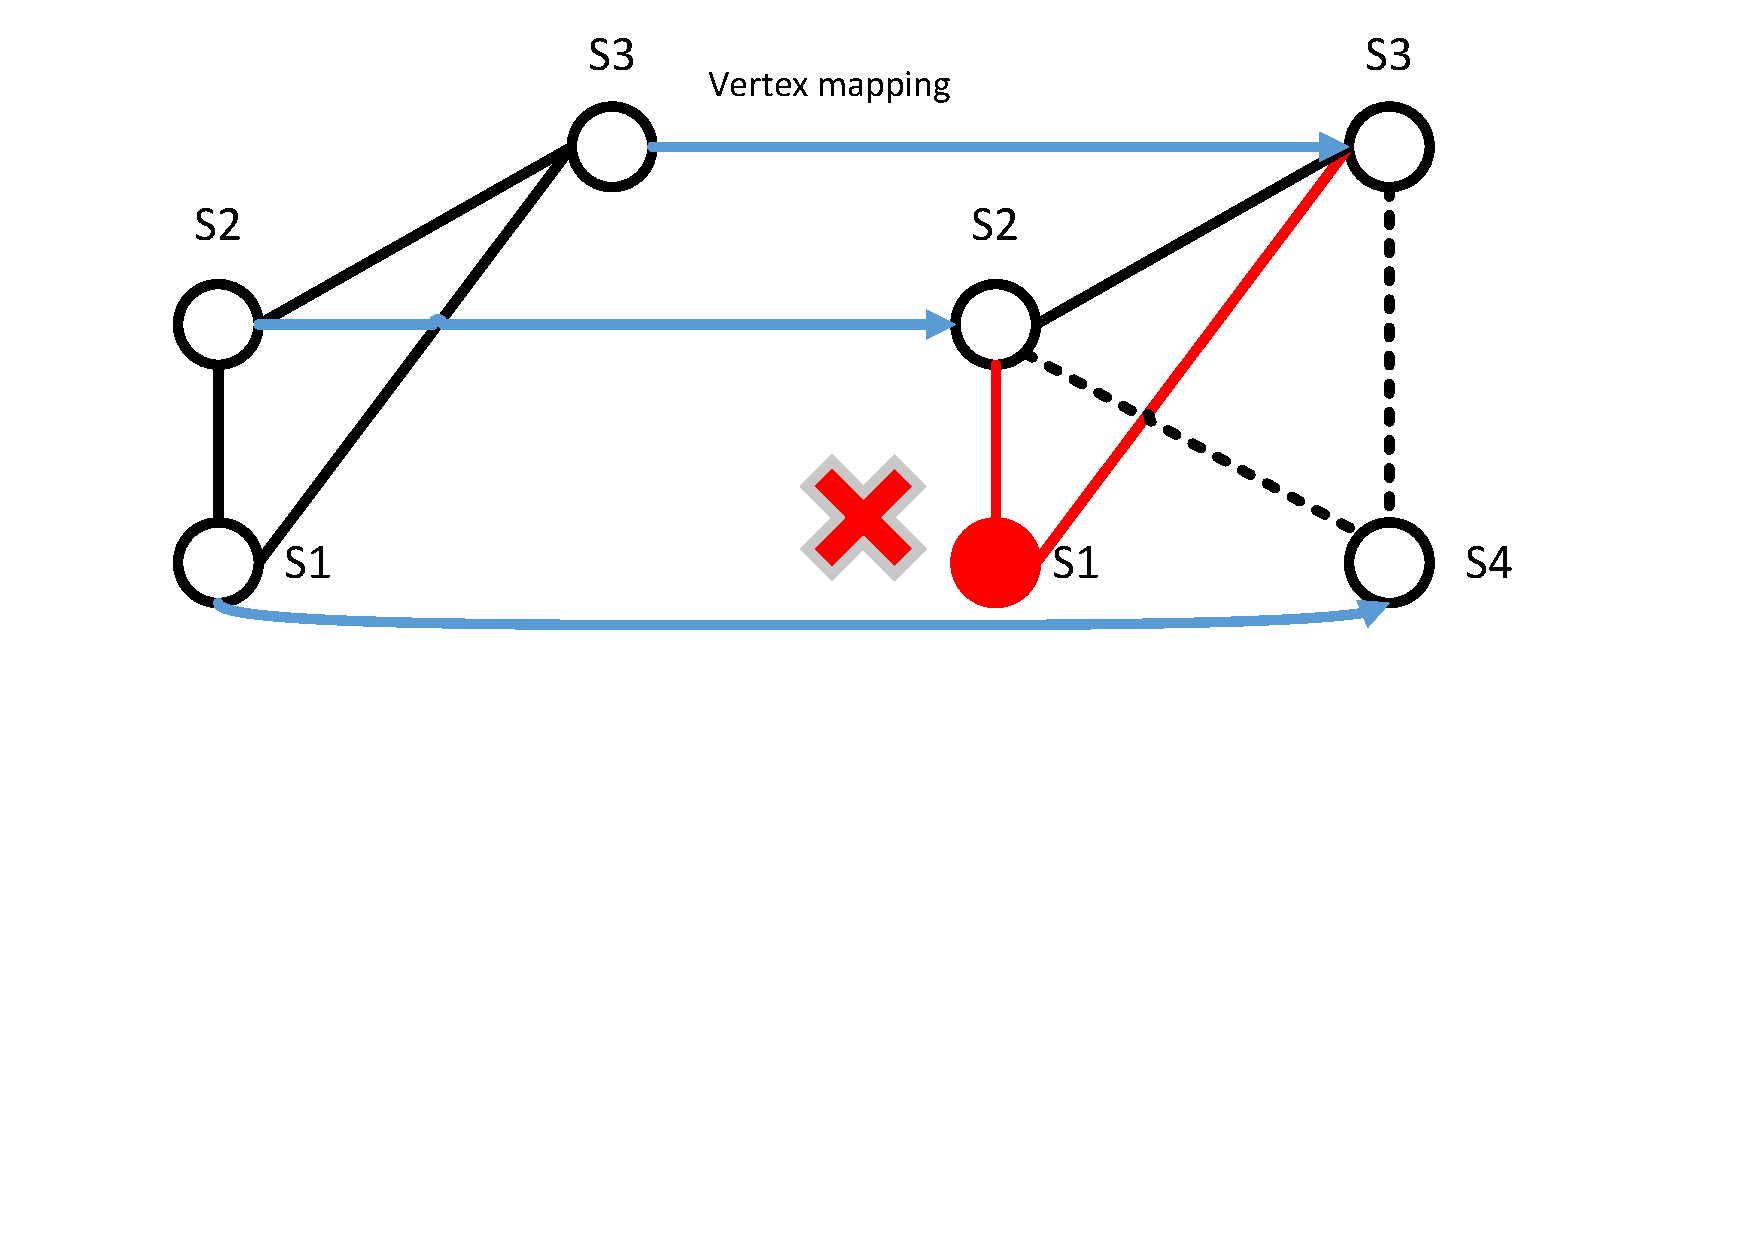
\includegraphics[width=1.5in]{Fig/MapA}\\
  \caption{MapA}\label{Fig:MapA}
\end{figure}

\begin{figure}
  \centering
  % Requires \usepackage{graphicx}
  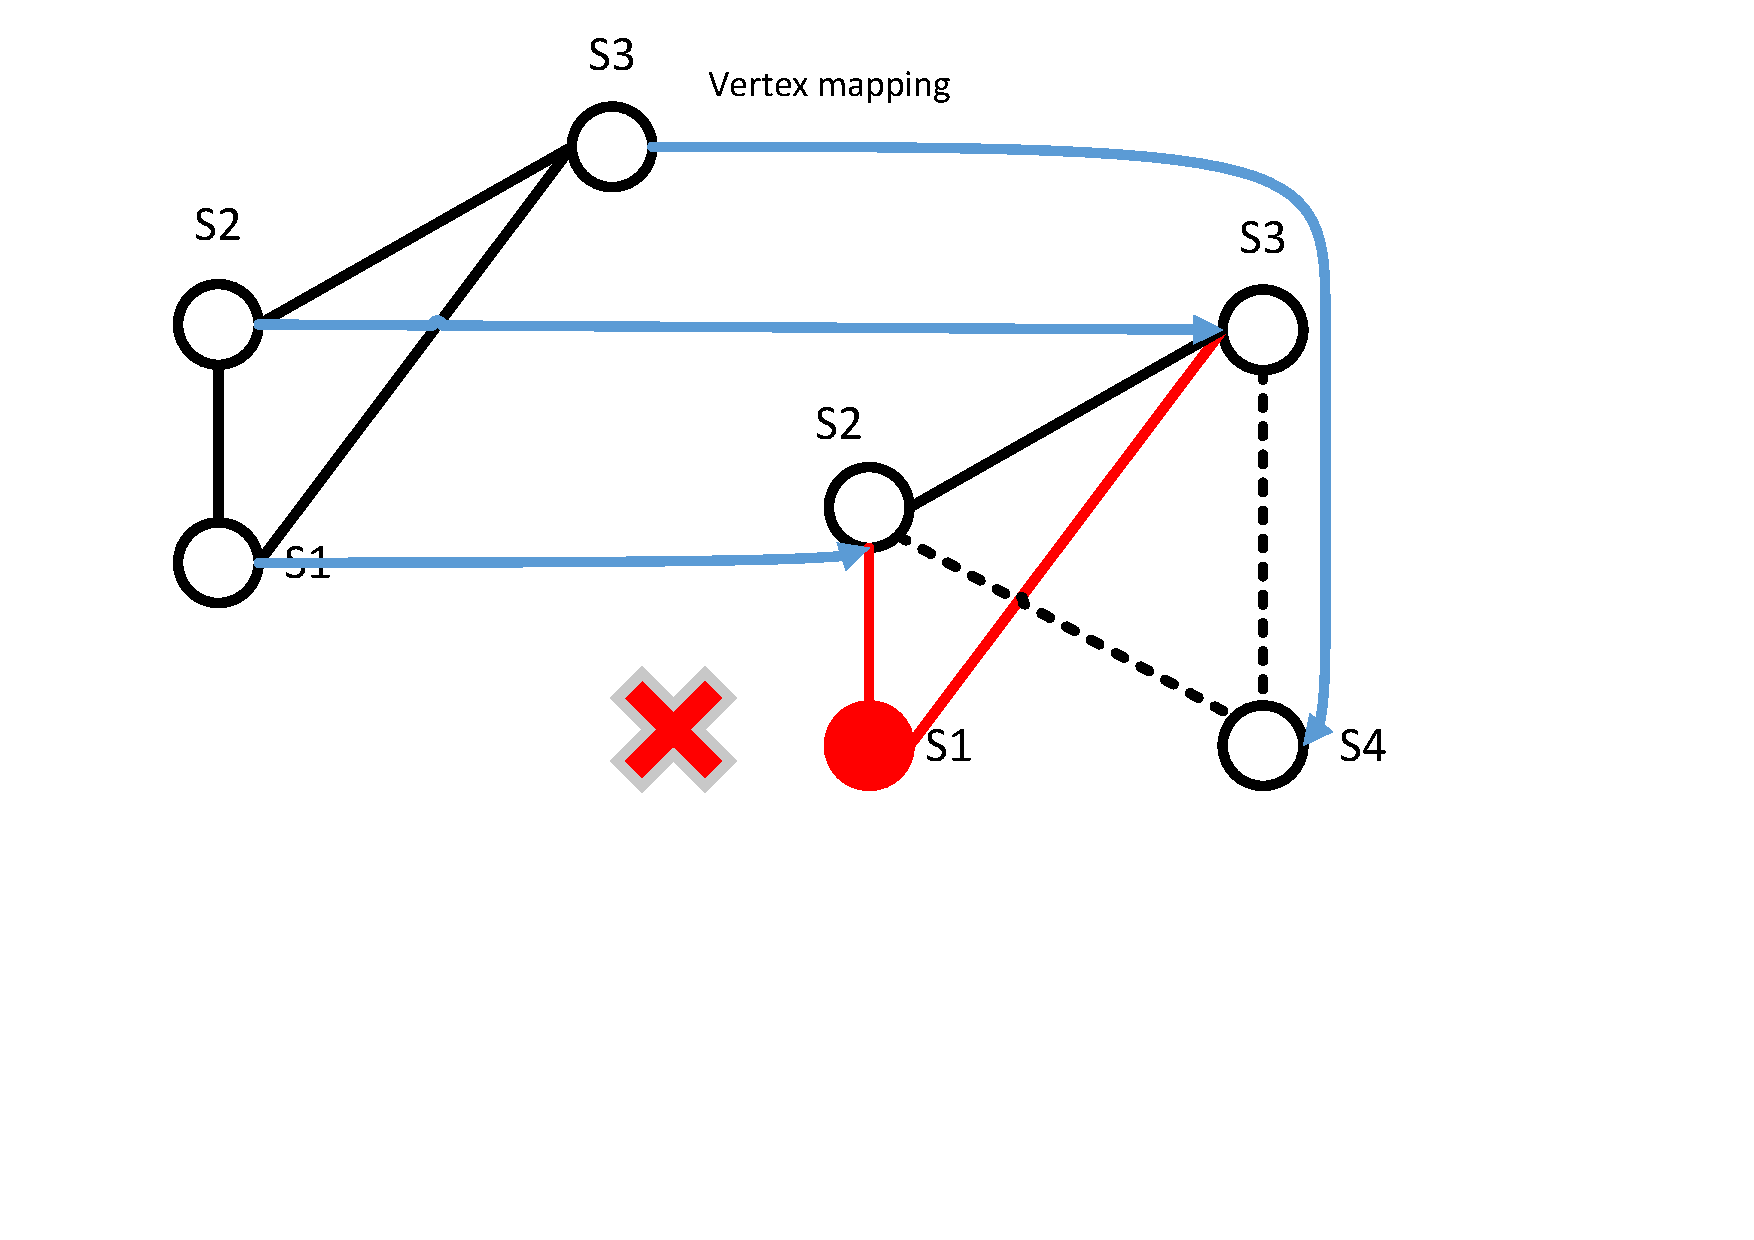
\includegraphics[width=1.5in]{Fig/MapB}\\
  \caption{MapB}\label{Fig:MapB}
\end{figure}



\begin{figure}
  \centering
  % Requires \usepackage{graphicx}
  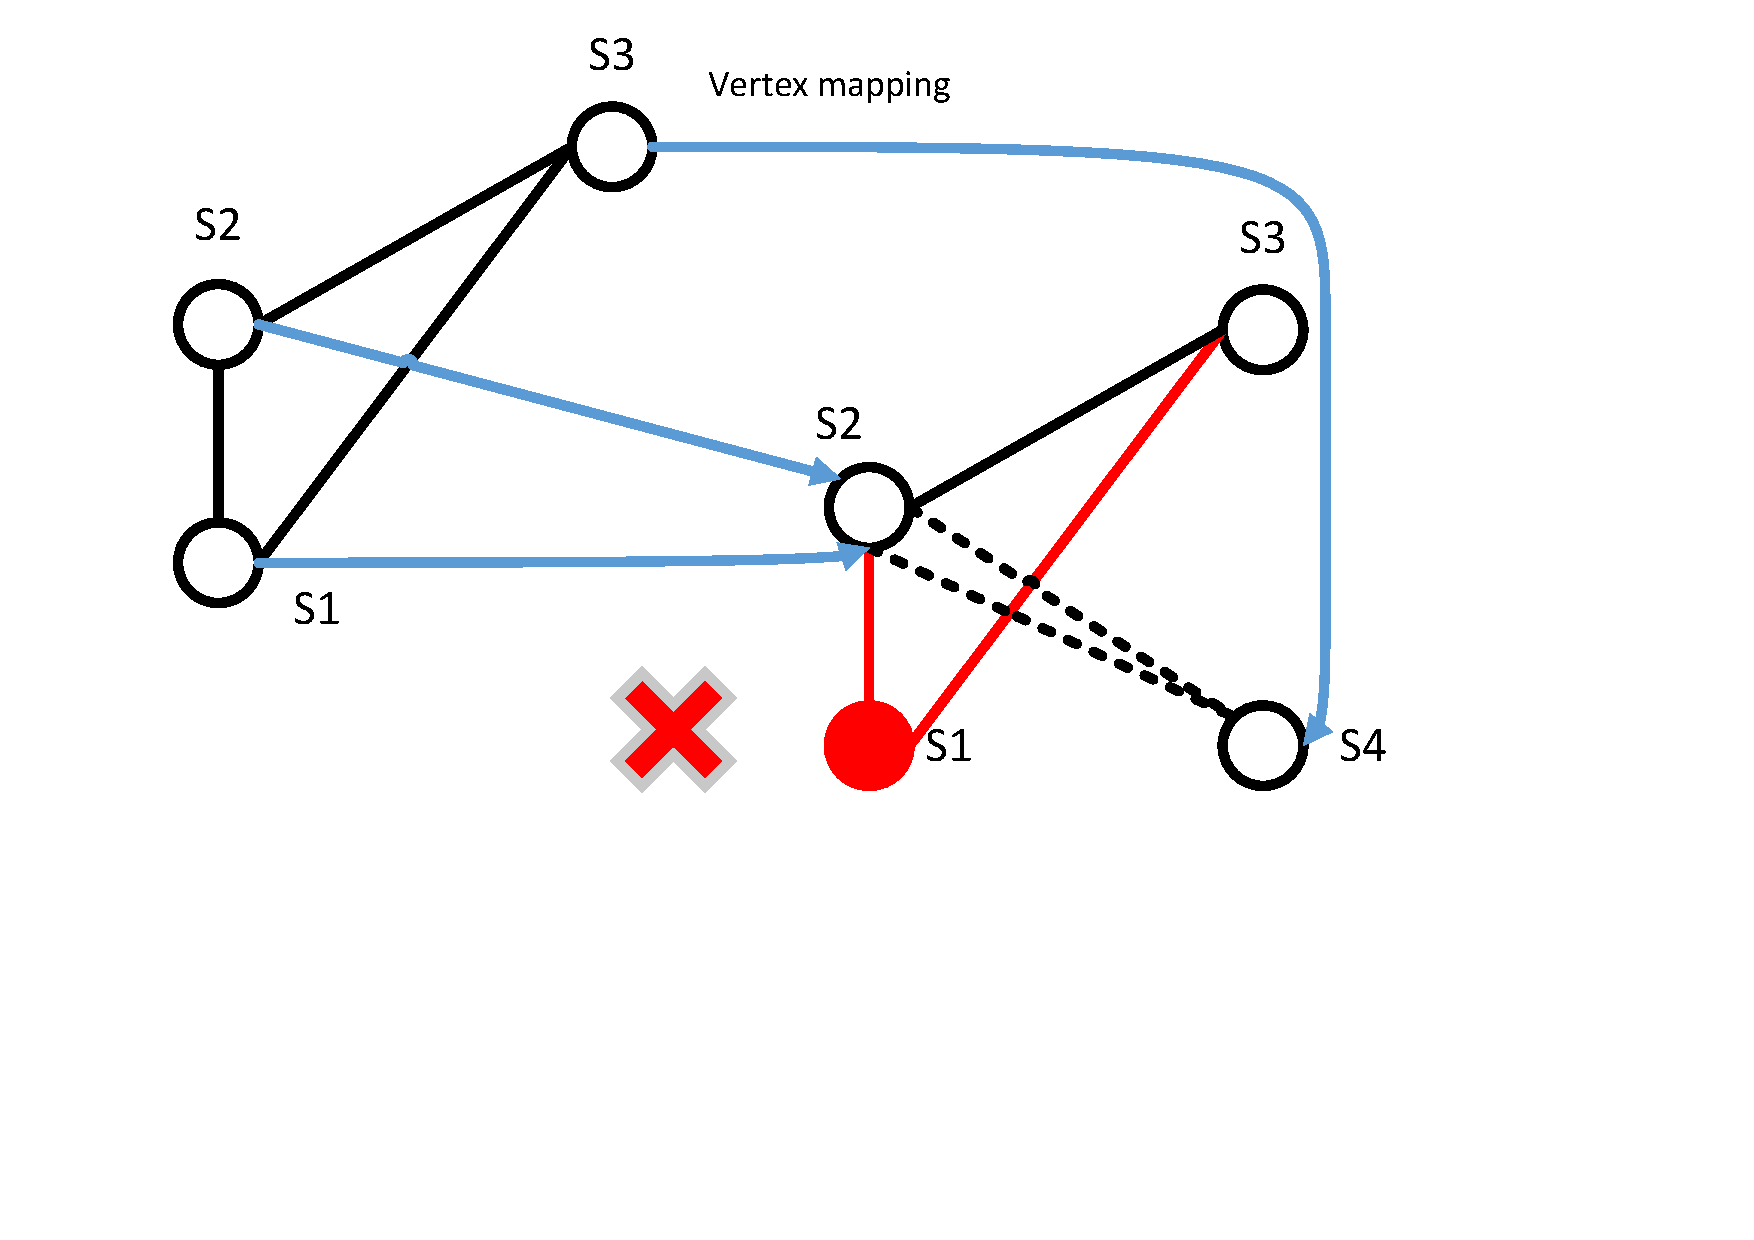
\includegraphics[width=1.5in]{Fig/MapC}\\
  \caption{MapC}\label{Fig:MapC}
\end{figure}

\begin{figure}
  \centering
  % Requires \usepackage{graphicx}
  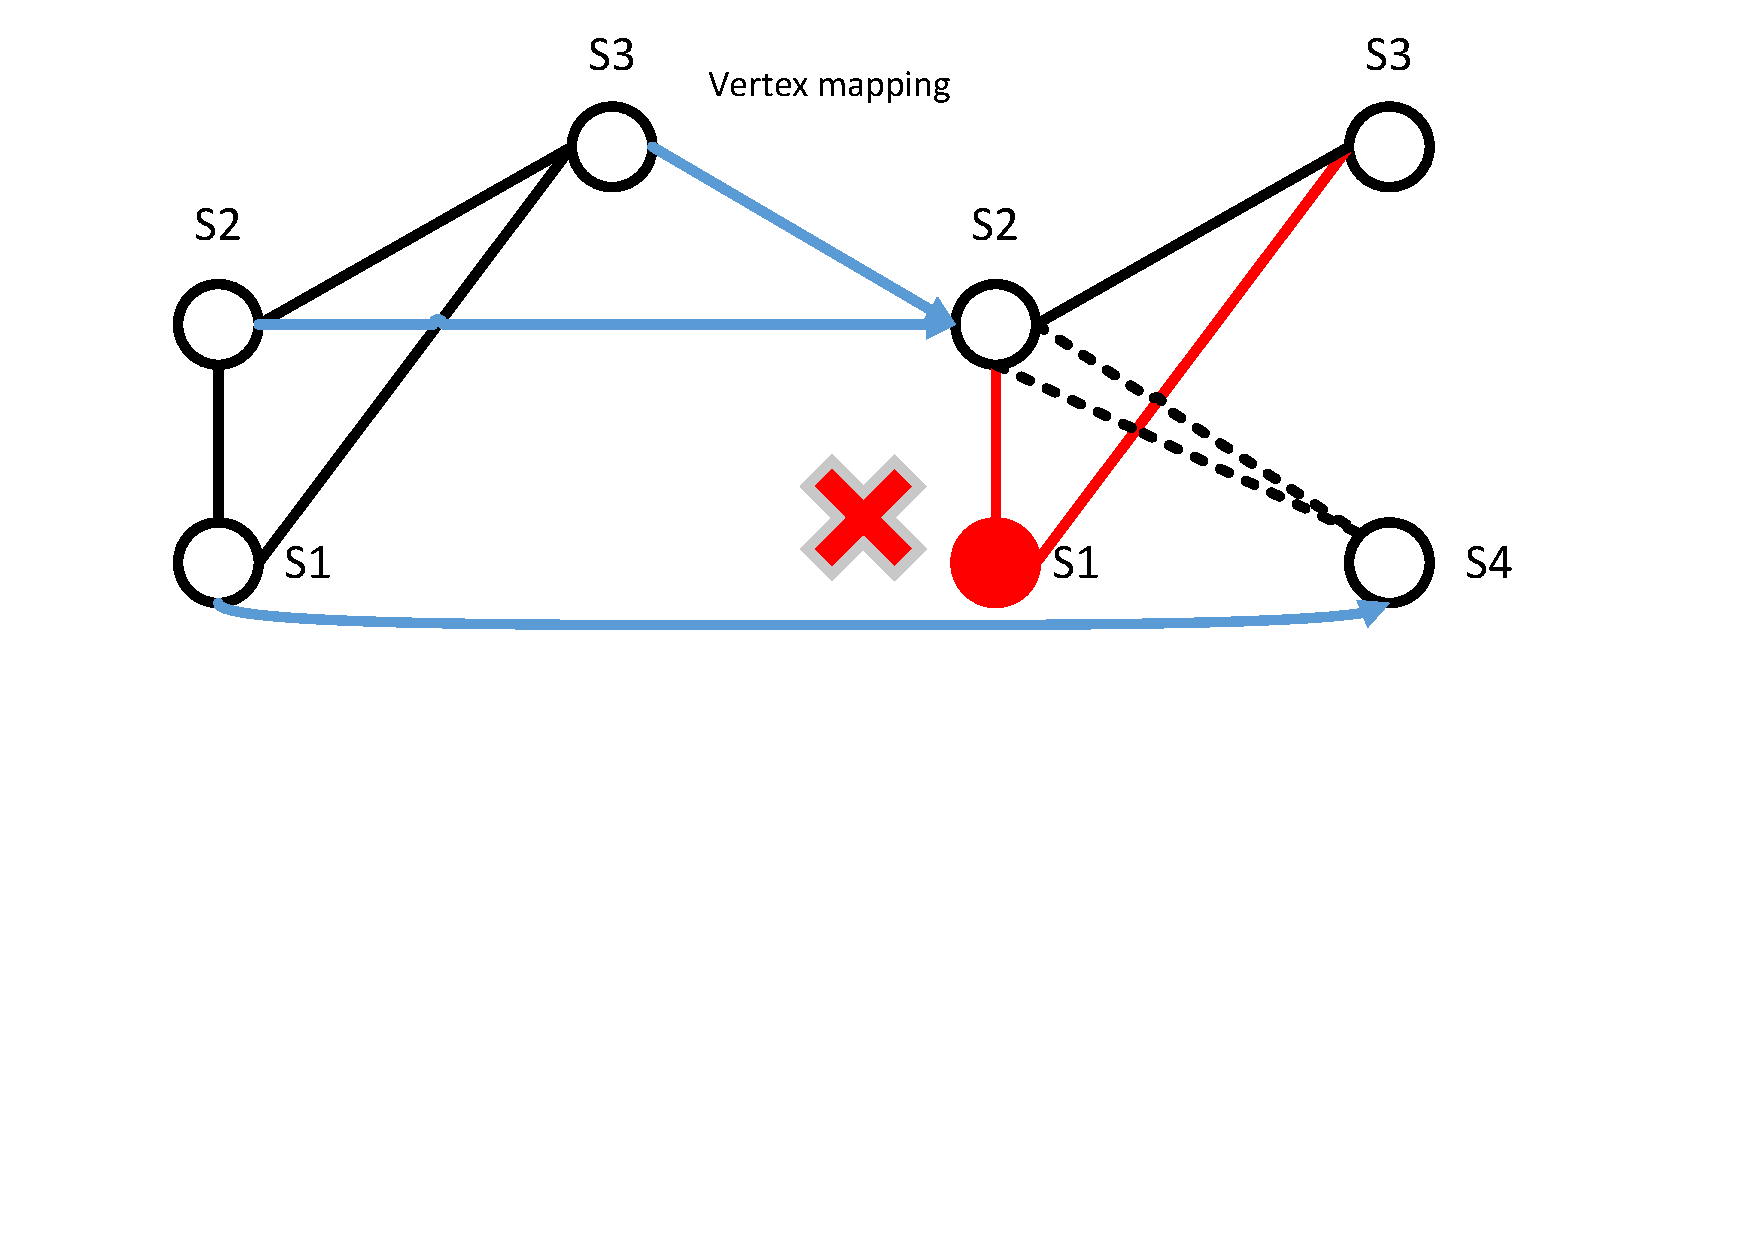
\includegraphics[width=1.5in]{Fig/MapD}\\
  \caption{MapD}\label{Fig:MapD}
\end{figure}


\begin{figure}
  \centering
  % Requires \usepackage{graphicx}
  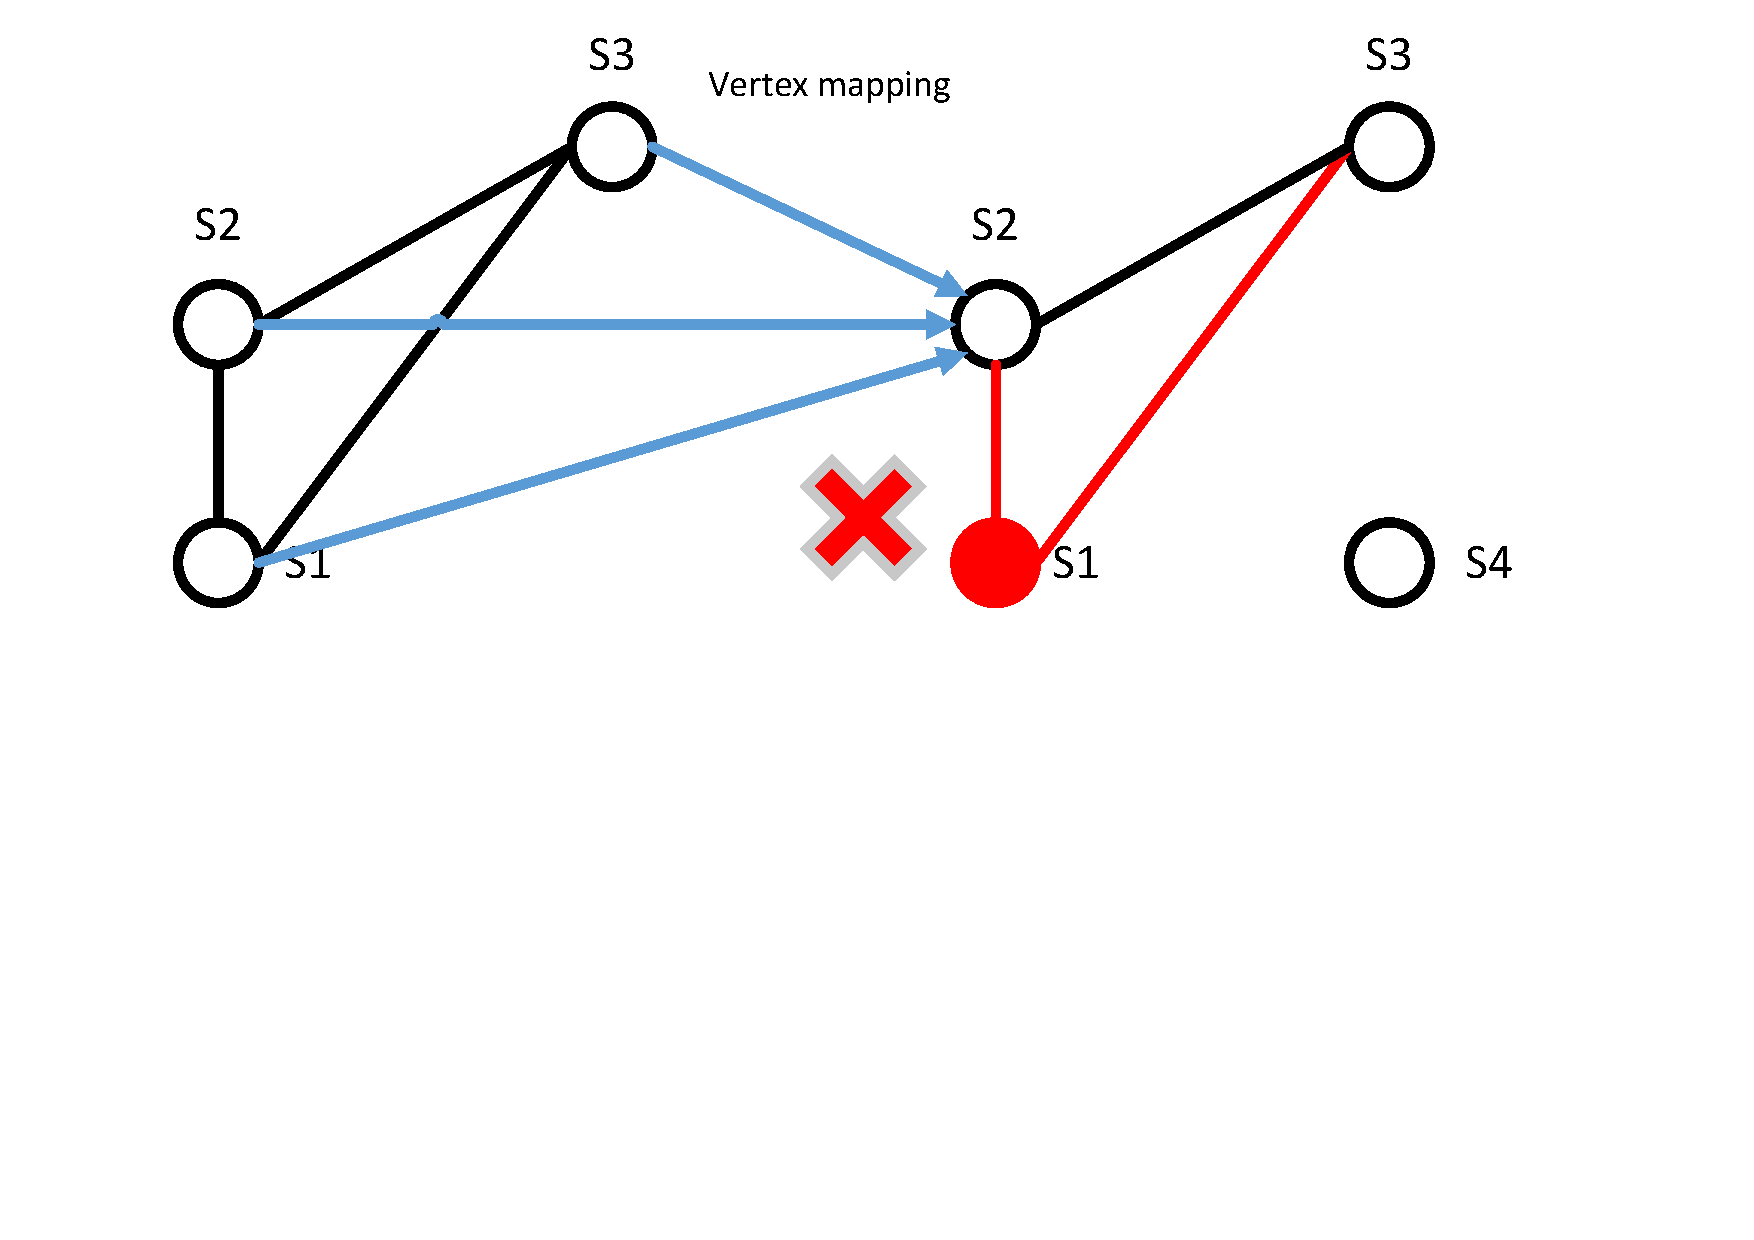
\includegraphics[width=1.5in]{Fig/MapE}\\
  \caption{MapE}\label{Fig:MapE}
\end{figure}


\section{Evaluation}
\label{sec:Evaluation}
We first described the simulation setup, then present the simulation results.

\subsection{Simulation setup}

\subsubsection{Experimental Parameter}
For any VN request, the number of VN nodes is randomly determined by a uniform distribution between $\VirtualNodeSizeMinimum$ and $\VirtualNodeSizeMaximum$ and each pair of virtual nodes is randomly connected with probability of $\VirtualNodenodeProbability$. The computing demand on VN nodes follow a uniform distribution from $\VirtualNodeComputationMinimum$ to $\VirtualNodeComputationMaximum$, as well as the bandwidth on VN links from $\VirtualEdgeBandwithMinimum$ to $\VirtualEdgeBandwithMaximum$.

%VN requests arrive randomly over a timespan of $\SubstrateNewtorkRunTimeInterval$ time slots and the inter-arrival time is
%assumed to follow the Geometric distribution at a rate of $\requestAppearProbability$ per time slot. The resource lease times of each VN request follows the uniform distribution as well at a rate  range from $\VNRequestsContinueTimeMinimum$ and $\VNRequestsContinueTimeMaximum$ per time slot.
The arrivals of VN requests are modeled by a Poisson process (with mean of \PossionMean \ requests per 1 time units).
The duration of the requests follows an exponential distribution with $\VNRequestsContinueTimeExponentialMean$ time units on average.
A high request rate and long lease time ensures that the physical infrastructure is operating at high utilization. we supposed a assumption that each virtual node of VN should be mapped on only one isolated physically substrate node.
%The arrivals of VN requests are modeled by a Poisson process (with mean of \PossionMean requests per 1 time units).
%The duration of the requests follows an exponential distribution with $\VNRequestsContinueTimeExponentialMean$ time units on average

We assumed the relative cost of computing demand  compared with bandwidth demand is $\RelativeCostbetweenComputingBandwidth$ according to  \cite{armbrust2009above,yu2010survivable}, which means $\lambda/\alpha=\RelativeCostbetweenComputingBandwidth$.
%The SN topologies used are randomly generated with $\SubStrateNodeSize$ nodes using the GT-ITM tool  \cite{zegura1996model}.
The SN topologies used from SNDlib topology data \cite{orlowski2010sndlib}as shown in Tab.\ref{tab:SNDlibTopo}.
The computing(bandwidth) resources of the substrate nodes (links) are integer uniformly distributed between $\SubStrateNodeComputationMinimum$ and $\SubStrateNodeComputationMaximum$ ($\SubStrateEdgeBandwithMinimum$ and $\SubStrateEdgeBandwithMaximum$), respectively. To model the facility node failure scenario, we choose all substrate facility nodes of substrate network to fail one by one, and statistically calculating migration frequency in every $\SubStrateFacilityNodeFailDuration$ time units.
\begin{table}[htb]
\centering
\caption{SNDlib topology data}\label{tab:SNDlibTopo}
\begin{tabular}{|c|c|c|}
  \hline
  % after \\: \hline or \cline{col1-col2} \cline{col3-col4} ...
  name & node & edge \\
  \hline
  cost266& 37& 57\\
  geant& 22& 36\\
  germany50& 50& 88\\
  giul39& 39& 172\\
  janos-us-ca& 39& 122\\
  janos-us& 26& 84\\
  nobel-eu& 28& 41\\
  norway& 27& 51\\
  pioro40& 40& 89\\
  ta1& 24& 55\\
  ta2& 65& 108\\
  zib54& 54& 81\\
  \hline

\end{tabular}
\end{table}

%In our proposed star decomposition method for $\MyProblemAbrreviation$ problem, we employ a proactive failure dependent protection(FD) based $\MyProblemAbrreviation$ problem design with sufficient redundancy before embedding process in order to conquer the limitation of existing work, which consider the redundancy within the embedding process and failure independent protection based migration approach in resource efficiency.

For performance comparisons, besides our scheme (named by $\MyAlgorithmMethodAbrreviation$), we also implemented other survivable algorithms $\SecondAlgorithmMethodAbrreviation$ \cite{yeow2011designing} as follows:
\begin{itemize}
  \item $\SecondAlgorithmMethodAbrreviation$ : algorithm connect links between backup and critical nodes, between backup and backup nodes, but not connect links between critical and critical nodes. critical node denote the former physical node which is embedded with virtual nodes. backup node denote the augmented nodes.
  \item $\FouthAlgorithmMethodAbrreviation$: When every node of substrate mapped with virtual node fail, a simple method is that augment a new node physical node for migrating the failure virtual node and connect new link with the failure link in terms of the failure physical node.
\end{itemize}

Moreover, We compare with a virtual network embedding algorithm\cite{liu2011completing} which is the embedding method when virtual network request firstly arrived, where VN do not have survivability requirement, and the virtual network embedding request (labeled $\ThirdAlgorithmMethodAbrreviation$) as a baseline to gauge the amount of augmented resources consumed for survivability, label "algorithm shared" or "algorithm Noshared" in experimental evaluation figures. We supposed that when a virtual network is embedded in substrate network, the successful survivable guarantee has been supposed  with respect to algorithm $\ThirdAlgorithmMethodAbrreviation$.

Based on the resource of substrate network whether shared or non-shared(dedicated) \cite{lu2006efficient}, we independently implement the two situation with respect to resource distribution pattern. The substrate resource corresponding augment backup demand of  every virtual network request with survivable guarantee  could be shared with each other. Dedicated means that for each virtual network a
complete backup network can be set up and backup resources are fully dedicated to the virtual networks and independent from each other. However, this is resource inefficient, since for each virtual resource that gets embedded a dedicated substrate entity is needed. In some cases it might also be acceptable to share and reuse the backup resources in order to reduce the footprint on the substrate network caused by the additional
backup resources. Usually, a higher degree of reused backup resources results in lower reliability, and vice versa.

Every virtual network's request exist a life lease time span, statistically record virtual or substrate network's performance metric in real-time situation. Because the experimental data of every algorithm's performance metric fluctuate, we incrementally record experimental data of every virtual or substrate network performance metric, then average the experimental data by successful accepted virtual network embedding or survivable embedded virtual network  as denominator.


All simulations ran on a server, which is equipped with Intel(R) Xeon(R) CPU E5-2620 2.00GHz (24 Cores) and 32.00GB RAM.

%one Intel (R) i5-5200U CPU(2.20GHz) (24Cores) and 8.00GB RAM.

\subsubsection{Performance Metric}
In this section, we evaluate the performance of the SeVN problem heuristic method $\MyAlgorithmMethodAbrreviation$ when allocating resources with considering all virtual nodes. In particular, we focus on the resource usage of the physical infrastructure and virtual network request, and the acceptable rates of survivable eVN  requests.

%The arrivals of VN requests are modeled by a Poisson process (with mean of 10 requests per 100 time units). The duration of the requests follows an exponential distribution with 1000 time units on average.

%The physical infrastructure consists of 40 compute nodes with capacity uniformly distributed between 50 and 100 units. These nodes are
%randomly connected with a probability of 0.4 occurring between any two nodes, and the
%bandwidth on each physical link is uniformly distributed between 50 and 100 units. VInf
%requests arrive randomly over a timespan of 800 time slots and the inter-arrival time is
%assumed to follow the Geometric distribution at a rate of 0.75 per time slot. The resource
%lease times of each VInf follows the Geometric distribution as well at a rate of 0.01 per time
%slot. A high request rate and long lease times ensures that the physical infrastructure is
%operating at high utilization. Each VInf consists of nodes between 2 to 10, with a compute
%capacity demand of 5 to 20 per node. Up to 90$\%$ of these nodes are critical and all failures
%are independent with probability 0.01. Connectivity between any two nodes in the VInf is
%random with probability 0.4, and the minimum bandwidth on any virtual link is 10 units.
%There are two main sets of results: (i) scaling the maximum bandwidth of a virtual link
%from 20 to 40 units while reliability guarantee of every VInf is 99.99$\%$, and (ii) scaling the
%reliability guarantee of each VInf from 99.5$\%$ to 99.995$\%$ while the maximum bandwidth
%of a virtual link is 30 units.


%The simulation experiments aim to assess the effect of substrate resource sharing among multiple priority classes and multiple vir- tual networks. Table 4 summarizes the settings for the simulation experiments. Random networks are considered to be the topology of the substrate networks [28] . In the random networks, a link is sequentially configured between each pair of nodes at the same probability. When random tree networks are considered to be the topology of the substrate networks, a substrate link is sequentially configured between each pair of substrate nodes at the same prob- ability under the condition that the addition of the new substrate link can avoid loop occurrence. Generation of the random networks is repeated until a connected graph is obtained as the topology of the substrate network. The number of virtual nodes in each requested virtual network follows a binomial distribution. The number of virtual nodes is more than one and less than or equal to the total number of sub- strate nodes. This means that the probability of the number of vir- tual nodes being vn ( > 1) can be given by the following expres- sion: P ( v n ) = P  ( v n ) /  | SN| v n  =2 P  v n  P  ( v n ) = | SN| C v n ( | V N| / | SN| ) v n ( 1 . 0 −| V N| / | SN| ) | SN| −v n (21) In the above expression, the notations | SN | and | VN | indicate the total number of substrate nodes and the average number of virtual nodes in each requested virtual network. A virtual link connects a pair of virtual nodes at a given probability P . However, each vir- tual node must be connected with at least one of the other virtual nodes using a virtual link. This means that the topology of the vir- tual networks is given by the connected random graph as with the substrate networks. Each priority class is evenly specified for each virtual link and pair of service components at both sides of the vir- tual link. The arrival of VNE requests follows the Poisson process and the lifetime of virtual networks follows a negative exponential distribution. Since the average lifetime of virtual networks is set at 1.0, the arrival rate of VNE requests is equal to the average number of virtual networks embedded simultaneously. For simplicity, the average traffic volume T is assumedto be 0.5 in every virtual link and service component, and the standard deviation of the traffic volume σ(T) is also identical in every vir- tual link and service component. Furthermore, the deviation part of the required amount of substrate resources k pr σ(T) is identical in every virtual link and service component belonging to the same priority class pr , and is given as shown in Table 4 . When the num- ber of priority classes is two, the deviation part is 0.8 in the low priority class and 1.2 in the high priority class. When the number of priority classes is four, the deviation part increases from 0.7 in the lowest priority class to 1.3 in the highest priority class. Then, the amount of substrate resources required for a set of m virtual links or service components that involves m pr virtual links or ser- vice components of each priority class pr is derived from expres- sions ( 2 ) and ( 3 ) as follows, when those m virtual links or service components share the substrate resource with each other: B = 0 . 5 m +  pr ( kpr σ(T ) ×√ mpr ) (22) Meanwhile, the amount of substrate resources required for a set of m virtual links or service components is derived from expression ( 4 ), when those m virtual links or service components cannot share the substrate resource: B = 0 . 5 m +  pr ( kpr σ(T ) ×mpr ) (23) It can be expected from expressions ( 22 ) and ( 23 ) that the ef- fect of substrate resource sharing strengthens due to the increase in the ratio of virtual links or service components belonging to higher priority classes, although the total required amount of sub- strate resources increases. However, the following simulation ex- periments specify the ratio such that the virtual links or service components of each priority class are distributed equally in order to estimate the effect of statistical multiplexing apart from the im- pact of the ratio. When the required amount of substrate resources is calculated, both the weights for the substrate link bandwidth W1 and sub- strate node capacity W2 are set at 1.0. In each simulation, the ini- tial interval for the first 50 0 0 virtual network requests is regarded as the transition state. The following interval for 10,0 0 0 virtual network requests is regarded as the stationary state and the statis- tics required are collected from the measurement results during the interval.


%Simulation settings.
%Setting item Setting value
%Topology of substrate network Random (tree) network
%Total number of substrate nodes (| SN |) 20, 100, 150, 201
%Total number of substrate links (| SL |) 30, 150, 200, 250
%Distribution of number of virtual nodes Binomial distribution
%Average number of virtual nodes (| VN |) 6 , 9,12
%Probability that a virtual link exists between a pair
%of virtual nodes ( P )
%0 .25, 0.50. 0.75
%Number of priority classes (| Pr |) 2, 4 (Each class
%specified evenly.)
%Arrival of virtual network requests Poisson process
%Average arrival rate of virtual network requests Variable parameter
%Lifetime of virtual networks Negative exponential
%distribution
%Average lifetime of virtual networks 1 .0
%Average traffic volume in each virtual link and
%service component ( T )
%0 .5
%Standard deviation of traffic volume for each
%virtual link and service component ( σ( T ))
%Constant
%Deviation part of substrate resource required for
%each virtual link and service component
%belonging to priority class pr ( k pr σ( T ))
%0.8, 1.2 when | Pr | = 2,
%0.7, 0.9, 1.1, 1.3 when
%| Pr | = 4
%Weight for the substrate link bandwidth ( W1 ) 1 .0
%Weight for the substrate node capacity ( W2 ) 1 .0
%Transition state interval in one simulation 50 0 0 requests
%Stationary state interval in one simulation 10,0 0 0 requests

Different measures \cite{fischer2013virtual} of heuristic algorithms are presented in this section in terms of average acceptance ratio, embedding stress, and other measures as described in the follow.

$A_{VN}$ denote at time t arrived virtual network request number. Fig.\ref{fig:VirNetReqSurNetReq} show that the successful number of virtual network request  embedded into physical network denoted as $A_{eVN}$ and the successful number of embedded virtual network survivable request after embed backup resource denoted as $A_{SeVN}$.

\begin{figure}
  \centering
  % Requires \usepackage{graphicx}
  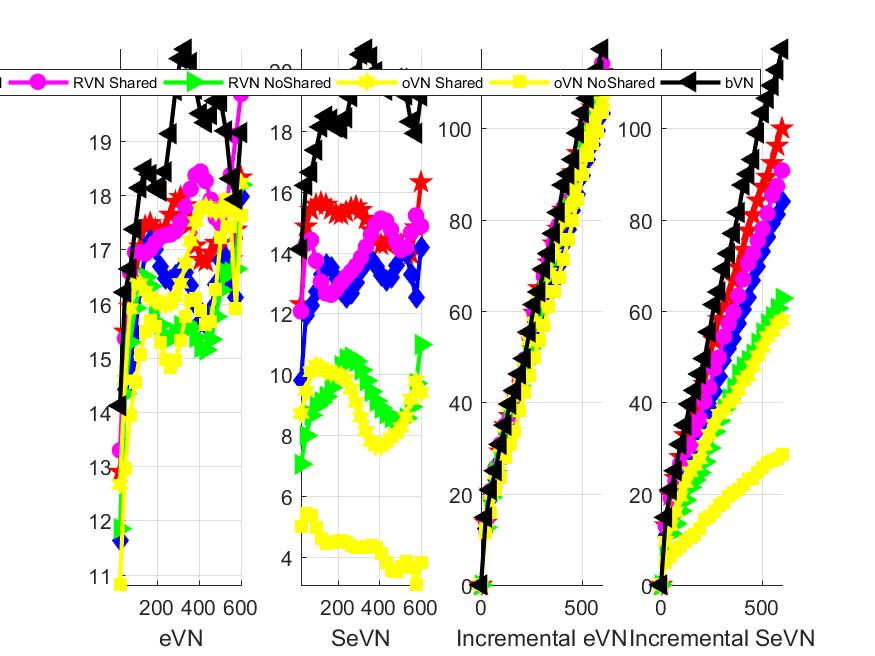
\includegraphics[width=3in]{Fig/VirNetReqSurNetReq}\\
  \caption{Accepted VNRs and Accepted SeVNRs}\label{fig:VirNetReqSurNetReq}
\end{figure}

\begin{itemize}
  \item \textbf{Acceptance Ratio}: Opposite to the concept of Blocking Probability. Ratio of a virtual network request is successful embedded into substrate network denoted as $A_{eVN}/A_{VN}$. Ratio of embedded virtual networks that were successfully augmented for survivable guarantees and embedded into the substrate topology denoted as $A_{SeVN}/A_{VN}$. Ratio of a embedded virtual network is successful survivable when the virtual network had been embedded in substrate network denoted as $A_{SeVN}/A_{eVN}$.
  \item \textbf{Active Node}, represent that number of substrate network booted nodes and number of survivable embedded virtual network request demand nodes. This metric is especially useful in the context of energy efficient VNE algorithms.
  \item \textbf{Path Length}: the path length metric measures the number of links between two interconnected virtual nodes, the number of links between two substrate nodes that are mapped to two interconnected virtual nodes.

  \item \textbf{Cost, Revenue, and Cost/Revenue}: Cost: Sum of node computing ability or link bandwidth resources being used for the embedding. Revenue: Sum of node computing ability or link bandwidth demands realized for the virtual networks. Cost/Revenue: The ratio indicates the virtualization overhead.
  \item \textbf{Stress}: Average number of virtual links/nodes that have been assigned to the substrate links/nodes .
 \item \textbf{Migration Frequency Ratio}: The number of migrations refers to the number of virtual nodes that need to be migrated to new facility nodes in case corresponding substrate nodes fail.
 \item \textbf{Utilization}: Bandwidth utilization or computing utilization of substrate links/nodes, in each SN entity (node or link), the sum of the spent substrate resources due to the mapping of virtual entities divided by the total amount of resources.
 \item \textbf{Backup nodes number}: The number of backups metric counts the number of backup resources that are set up for a virtual entity. Several additional substrate entities can be reserved to serve as a replacement in case the entity hosting the virtual entity fails.
\end{itemize}
%\begin{table*}
%\label{tab:measure}
%  \centering
%  \begin{tabular}{ll}
%    \fbox{Accepted SeVN Ratio} & Ratio of embedded virtual networks that were successfully augmented and embedded into the substrate topology \\
%    \fbox{Stress} & NO Average number of virtual links/nodes that have been assigned to the substrate links/nodes \\
%    \fbox{Utilization}& Bandwidth/CPU utilization of substrate links/nodes.\\
%    \fbox{Cost, Revenue, and Cost/Revenue}& Cost: Sum of CPU and bandwidth resources being used for the embedding. Revenue: Sum of CPU and bandwidth demands realized for the virtual networks. Cost/Revenue: The ratio indicates the virtualization overhead.\\
%    \fbox{Active Nodes} &Number of nodes that need to be active in order to host all the virtual networks. This metric is especially useful in the context of energy efficient VNE algorithms.\\
%    Path Length & NO Length of communication paths assigned to virtual links\\

%    Power Consumption &Power consumption of all Active nodes. Several power consumption models are implemented.\\
%    Runtime & Average runtime of the algorithm.\\
%    Initialization Overhead &Some algorithms come with initialization cost (in terms of runtime), e.g., the distributed algorithm presented in initially partitions the network before embedding VNRs.\\
%    Hidden Hops Ratio& Ratio of hidden hops, e.g., the number of nodes only needed for forwarding packages between other nodes. Especially useful in the context of energy efficient VNE algorithms.\\
%    Communication Overhead &Communication overhead of distributed algorithms (i.e., number of messages sent between substrate nodes).
%  \end{tabular}
%\end{table*}




\subsection{Acceptance Ratio}
In this section, acceptance ratio of the embedded VN's survivable request with respect to $\MyProblemAbrreviation$ problem. Moreover, the acceptance ratio of VN without survivability requirement is presented as a baseline to gauge the impact of additional amount of resources consumed for survivability on the service provisioning capability of SN.

In Fig.\ref{fig:AcceptionRatio}, acceptance ratio drops quickly before 200 time units because there are not sufficient substrate resources for the arrived VN requests. when the amount of running VN requests in system are stable after 400 time units, acceptance ratio would keep consistent. Fig.\ref{fig:AcceptionRatio} also depicts that $\MyAlgorithmMethodAbrreviation$ lead to higher acceptance ratio than $\SecondAlgorithmMethodAbrreviation$ algorithm needless of resources sharing. In particular, comparing with $\SecondAlgorithmMethodAbrreviation$-Shared, $\MyAlgorithmMethodAbrreviation$-Shared approach achieves almost 6\% improvement of acceptance ratio in the long run. Intuitively, it is the result of fact that, for $\MyAlgorithmMethodAbrreviation$-NoShared embedding, the backup node is associated with a lot of resources since it has to emulate every primary node after it fails, and so, embedding of backup node is vulnerable. However, the acceptance ratio suffers at least 6\% losses than $\MyAlgorithmMethodAbrreviation$-Shared caused by redundant resources consumption for survivability purpose.

\begin{figure}[htbp]
  \centering
  % Requires \usepackage{graphicx}
  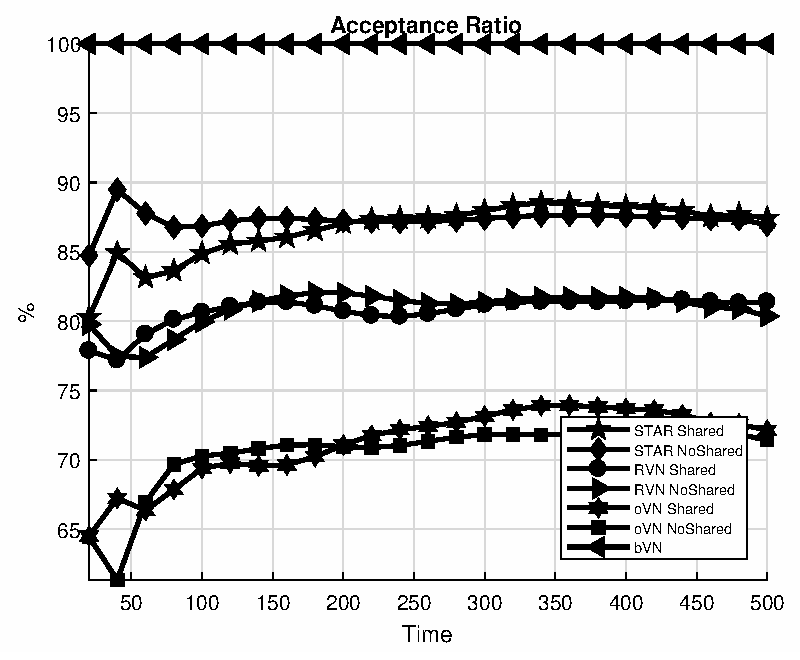
\includegraphics[width=3in]{Fig/AcceptionRatio}\\
  \caption{Acceptance Ratio}\label{fig:AcceptionRatio}
\end{figure}
\subsection{Active Node}
\subsubsection{Virtual Network Active Node}
Number of nodes that need to be active and embedded in order to host all the virtual networks.

Virtual Network Active Node Fig.\ref{fig:ActiveNodeVirtualNetwork}:
\begin{figure}[htbp]
  \centering
  % Requires \usepackage{graphicx}
  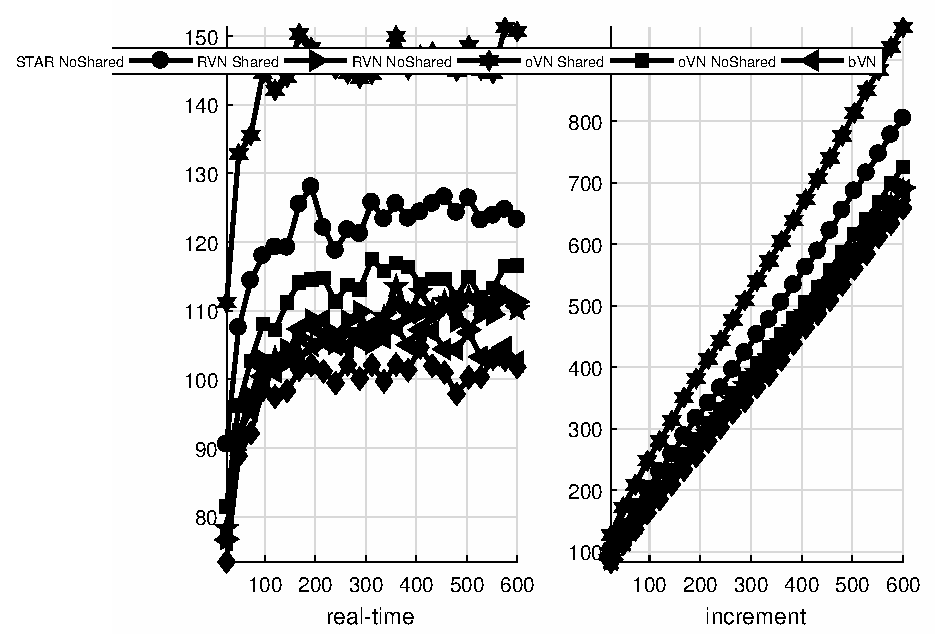
\includegraphics[width=3in]{Fig/ActiveNodeVirtualNetwork}\\
  \caption{Virtual Network Active Node}\label{fig:ActiveNodeVirtualNetwork}
\end{figure}

Virtual Network Average Active Node Fig.\ref{fig:ActiveNodeAverageVirtualNetwork}:
\begin{figure}[htbp]
  \centering
  % Requires \usepackage{graphicx}
  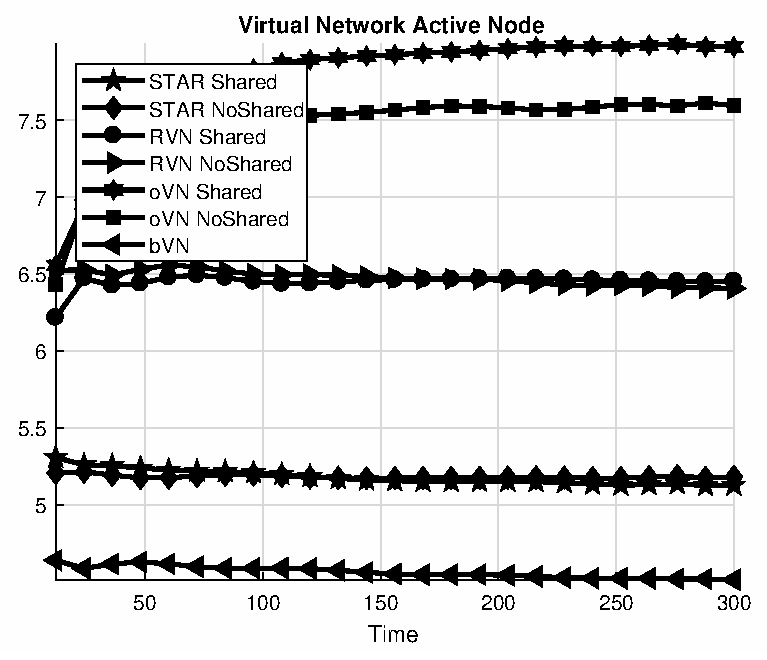
\includegraphics[width=3in]{Fig/ActiveNodeAverageVirtualNetwork}\\
  \caption{Virtual Network Average Active Node}\label{fig:ActiveNodeAverageVirtualNetwork}
\end{figure}

\subsubsection{Substrate Network Active Node}
The number of active substrate nodes is related to the average length of substrate paths, because additional nodes are used to forward communication data between end nodes. Therefore, the probability that previously switched off nodes are selected to forward data rises. Regarding energy efficiency, the number of nodes that need to be turned for an embedding can be a rough estimation of energy consumption.

Substrate Network Active Node Fig.\ref{fig:ActiveNodeSubstrateNetwork}:
\begin{figure}[htbp]
  \centering
  % Requires \usepackage{graphicx}
  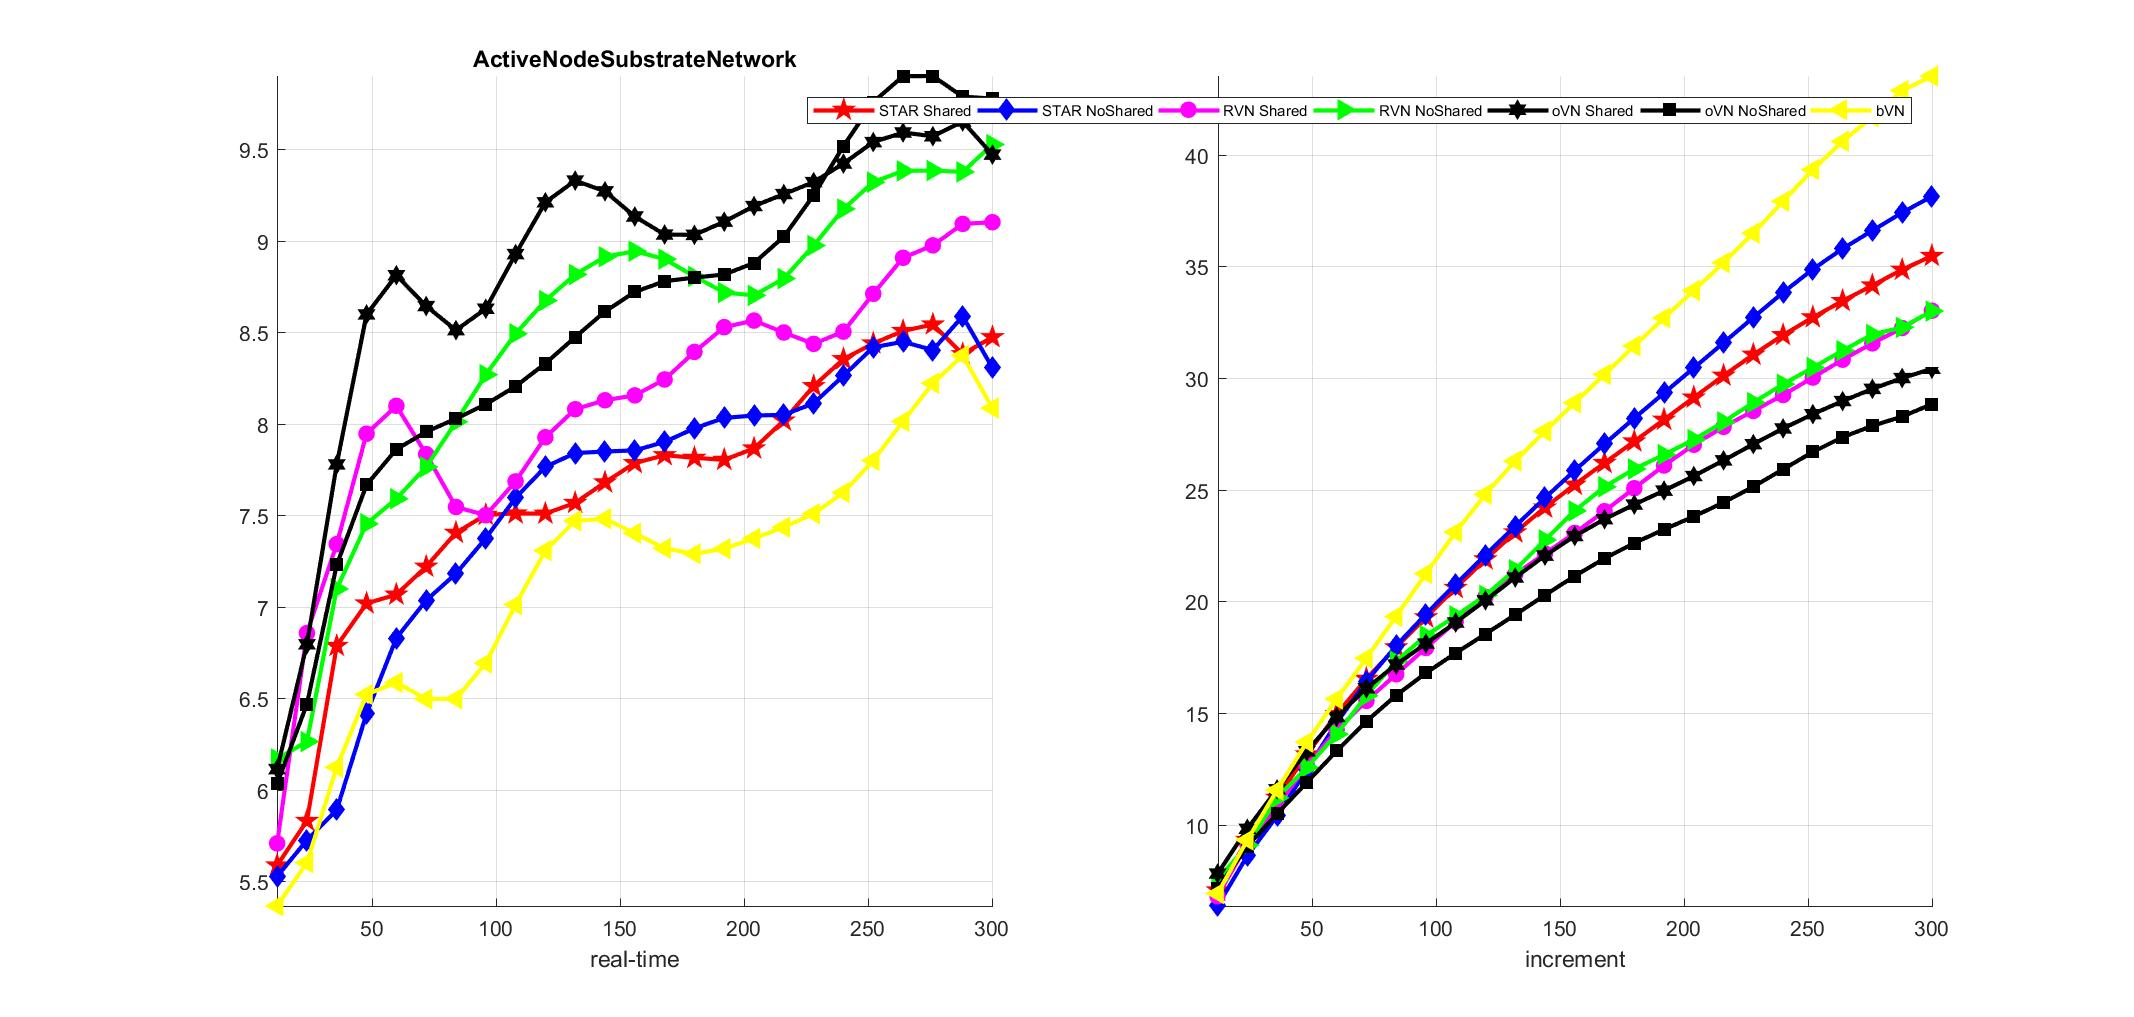
\includegraphics[width=3in]{Fig/ActiveNodeSubstrateNetwork}\\
  \caption{Substrate Network Active Node}\label{fig:ActiveNodeSubstrateNetwork}
\end{figure}


Substrate Network Average Active Node Fig.\ref{fig:ActiveNodeAverageSubstrateNetwork}:
\begin{figure}[htbp]
  \centering
  % Requires \usepackage{graphicx}
  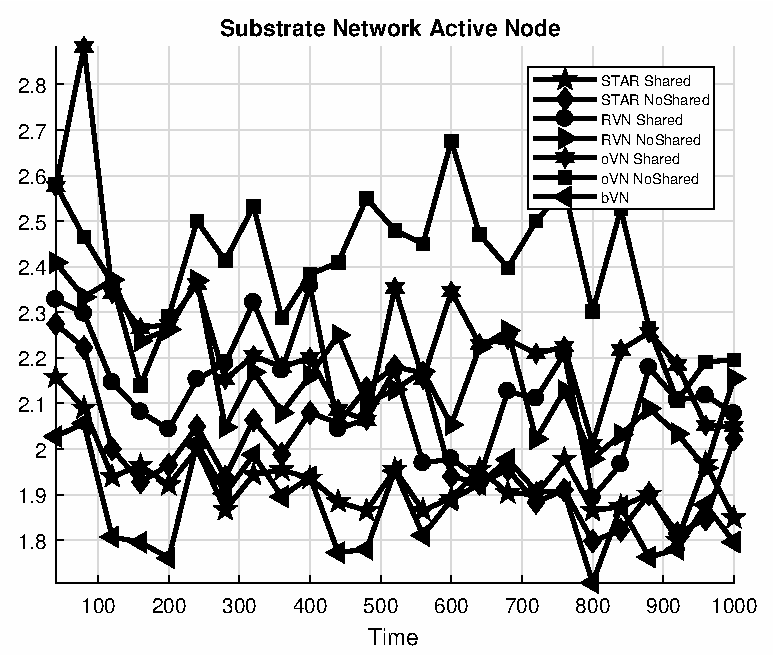
\includegraphics[width=3in]{Fig/ActiveNodeAverageSubstrateNetwork}\\
  \caption{Substrate Network Average Active Node }\label{fig:ActiveNodeAverageSubstrateNetwork}
\end{figure}

\subsubsection{Substrate Network Active Node/ Virtual Network Active Node }
In general, the ratio between running nodes and the total number of substrate nodes should be taken into account.

Substrate Network Active Node/ Virtual Network Active Node Fig.\ref{fig:ActiveNodeSubVir2VirNet}:
\begin{figure}[htbp]
  \centering
  % Requires \usepackage{graphicx}
  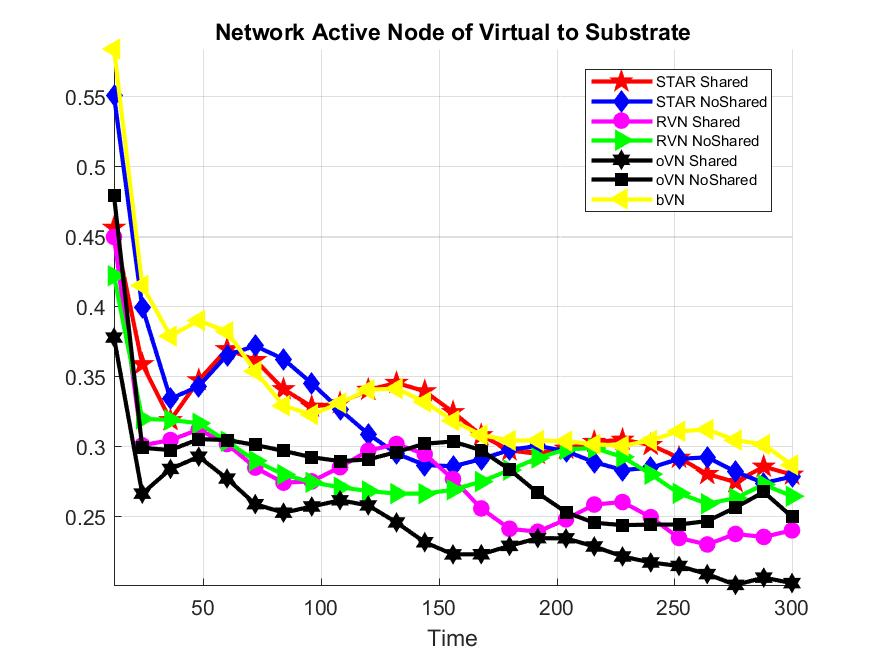
\includegraphics[width=3in]{Fig/ActiveNodeSubVir2VirNet}\\
  \caption{Substrate Network Active Node / Virtual Network Active Node}\label{fig:ActiveNodeSubVir2VirNet}
\end{figure}

\subsection{Path Length}
\subsubsection{Virtual network Path Length}

Virtual Network Path Length Fig.\ref{fig:PathLengthVirtualNetwork}
\begin{figure}[htbp]
  \centering
  % Requires \usepackage{graphicx}
  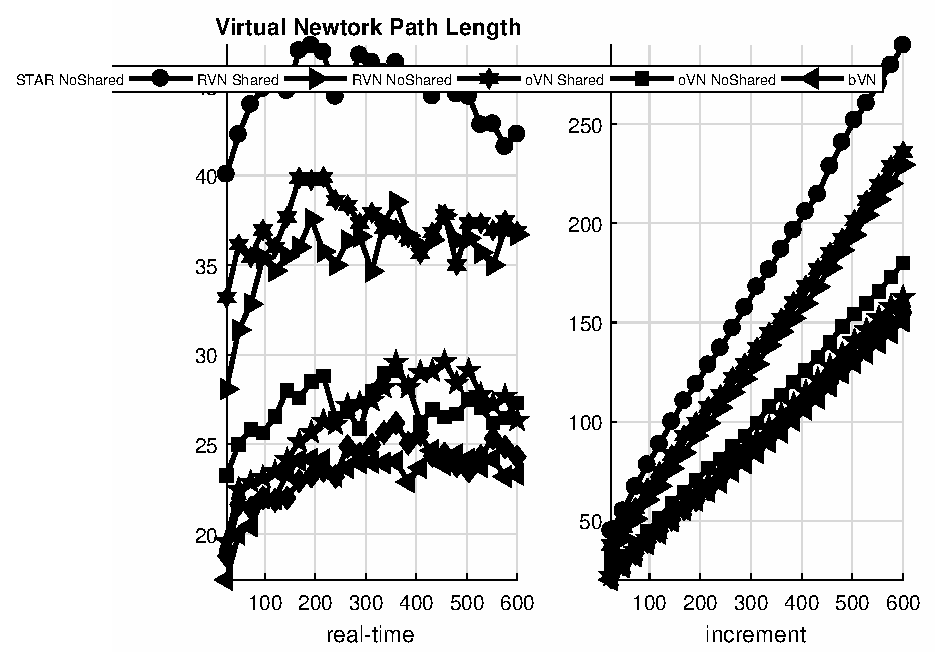
\includegraphics[width=3in]{Fig/PathLengthVirtualNetwork}\\
  \caption{ Virtual Network Path Length}\label{fig:PathLengthVirtualNetwork}
\end{figure}


Virtual Network Average Path Length Fig.\ref{fig:PathLengthAverageVirtualNetwork}:
\begin{figure}[htbp]
  \centering
  % Requires \usepackage{graphicx}
  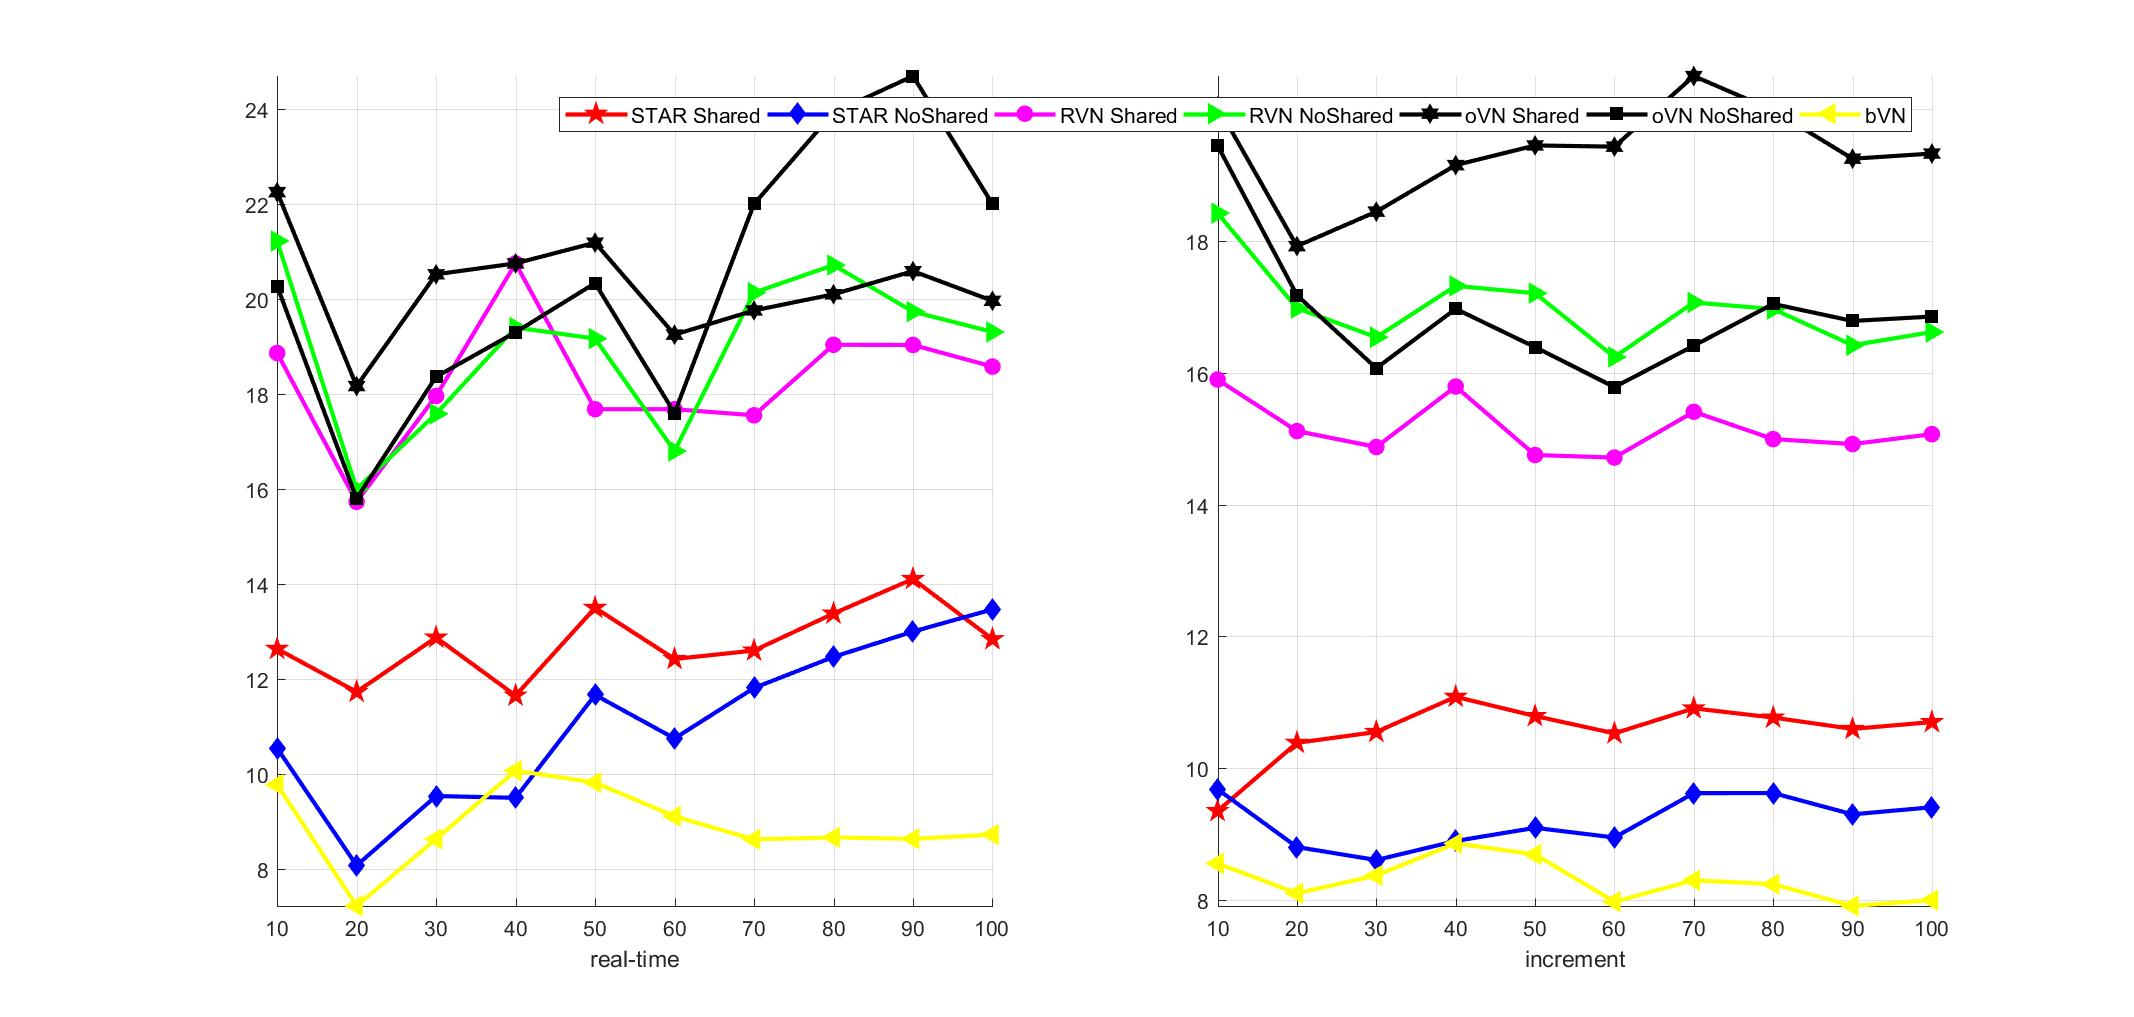
\includegraphics[width=3in]{Fig/PathLengthAverageVirtualNetwork}\\
  \caption{Virtual Network Average Path Length }\label{fig:PathLengthAverageVirtualNetwork}
\end{figure}

\subsubsection{Substrate network Path Length}
The longer a corresponding path, the more resources had to be reserved for the embedding of the virtual link. Since every substrate node (except the receiving node) that is part of a path will take some time to forward packages sent via this path, the quality of service is influenced by the path length. In general, the package delay increases in connection with the length of a path.

Substrate Network Path Length Fig.\ref{fig:PathLengthSubstrateNetwork}.
\begin{figure}[htbp]
  \centering
  % Requires \usepackage{graphicx}
  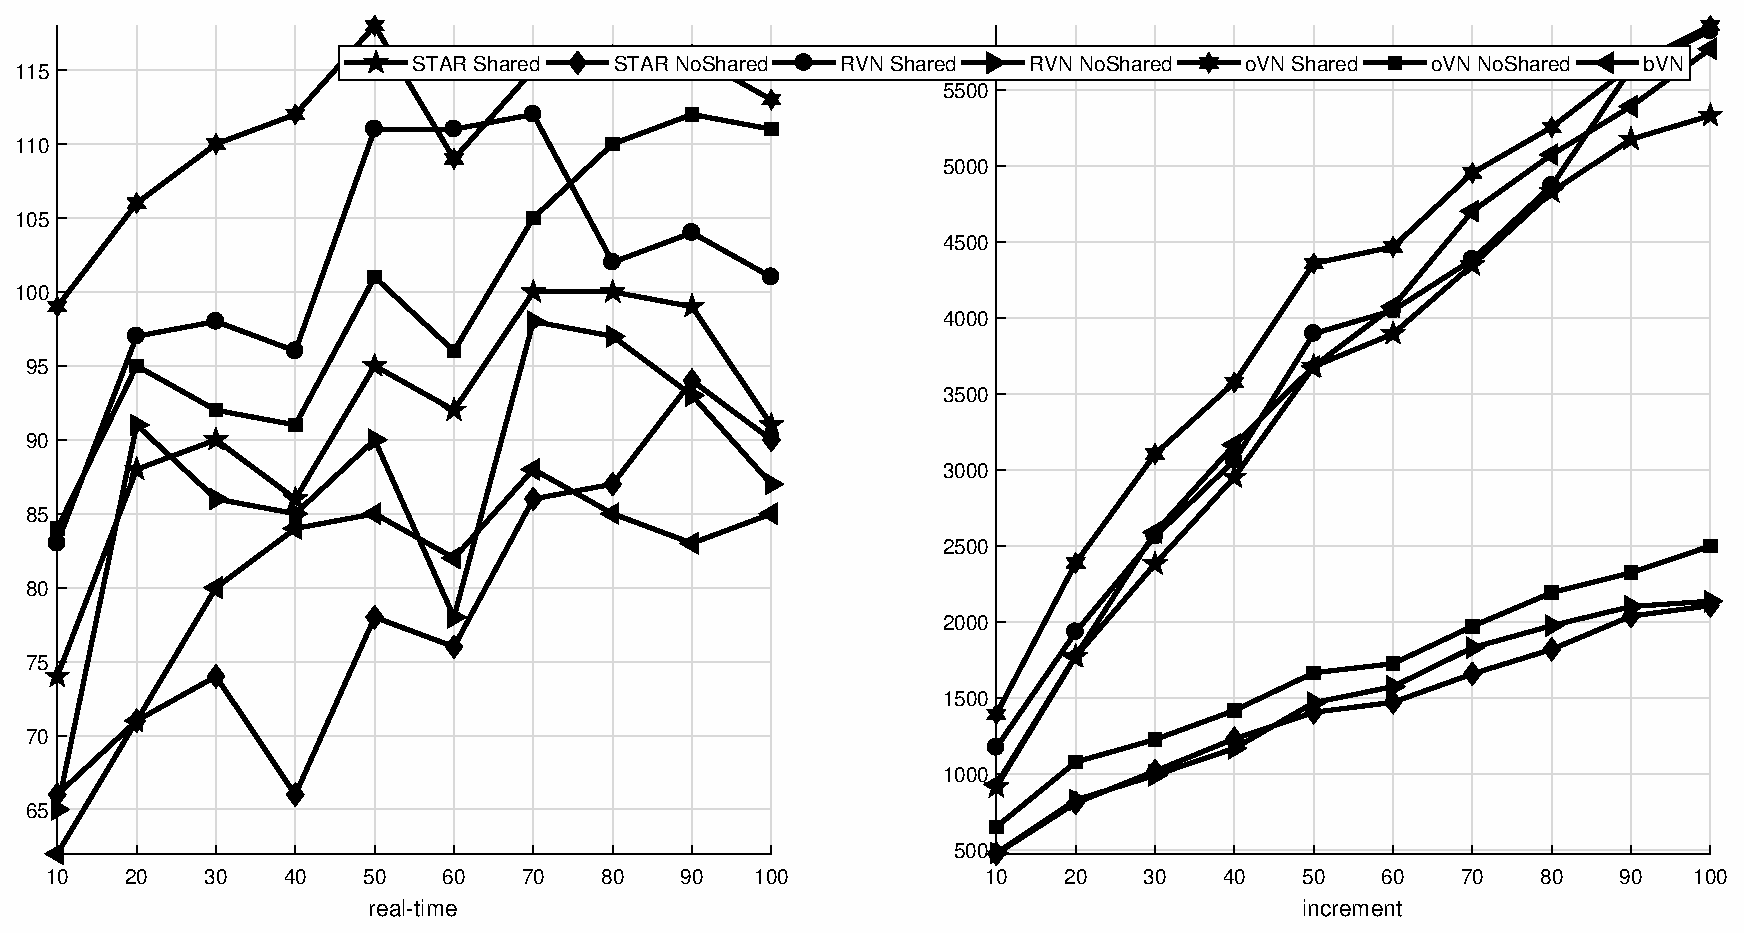
\includegraphics[width=3in]{Fig/PathLengthSubstrateNetwork}\\
  \caption{ Substrate Network Path Length}\label{fig:PathLengthSubstrateNetwork}
\end{figure}

Substrate Network Average Path Length Fig.\ref{fig:PathLengthAverageSubstrateNetwork}.
\begin{figure}[htbp]
  \centering
  % Requires \usepackage{graphicx}
  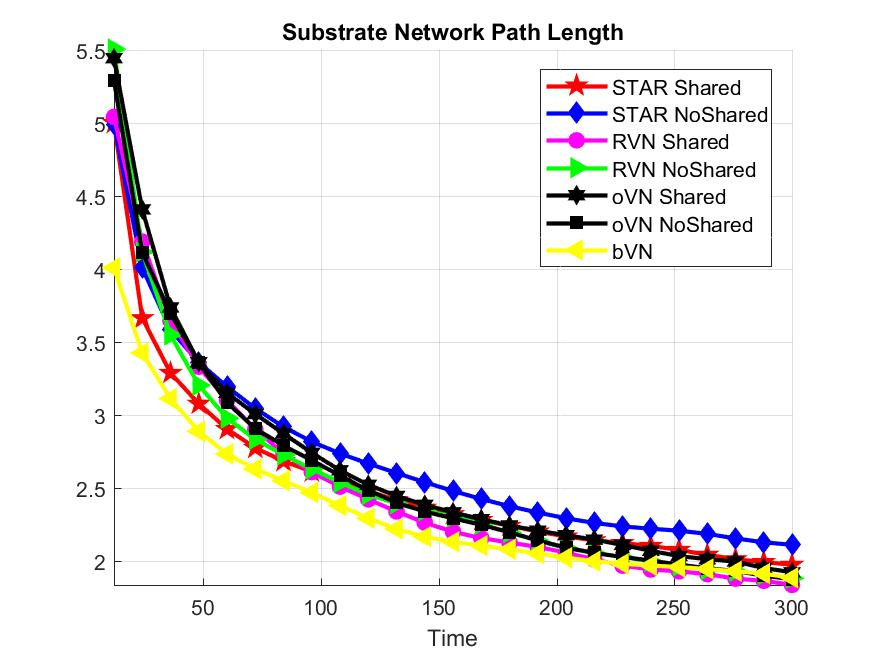
\includegraphics[width=3in]{Fig/PathLengthAverageSubstrateNetwork}\\
  \caption{ Substrate Network Average Path Length }\label{fig:PathLengthAverageSubstrateNetwork}
\end{figure}




\subsubsection{Substrate Network Path Length/ Virtual Network Path Length}


Substrate Network Path Length/ Virtual Network Path Length Fig.\ref{fig:PathLengthSubVir2VirNet}:
\begin{figure}[htbp]
  \centering
  % Requires \usepackage{graphicx}
  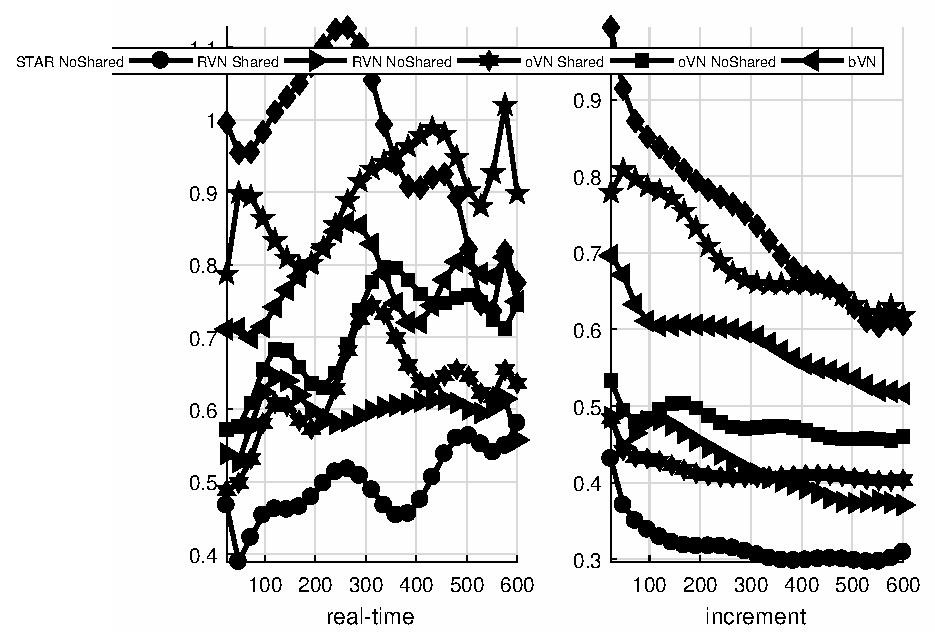
\includegraphics[width=3in]{Fig/PathLengthSubVir2VirNet}\\
  \caption{Substrate Network Path Length/ Virtual Network Path Length }\label{fig:PathLengthSubVir2VirNet}
\end{figure}



\subsection{Cost, Revenue and Cost/Revenue}
\subsubsection{Cost}
In this work, the embedding cost is calculated as the cost of the substrate resources (i.e. cost of node computing ability on all facility nodes, edge bandwidth on all fiber links) consumed to satisfy the $\MyProblemAbrreviation$ resource requirements.

Substrate Network Real-Time Cost Fig.\ref{fig:CostCurrentSubstrateNetwork}:
\begin{figure}[htbp]
  \centering
  % Requires \usepackage{graphicx}
  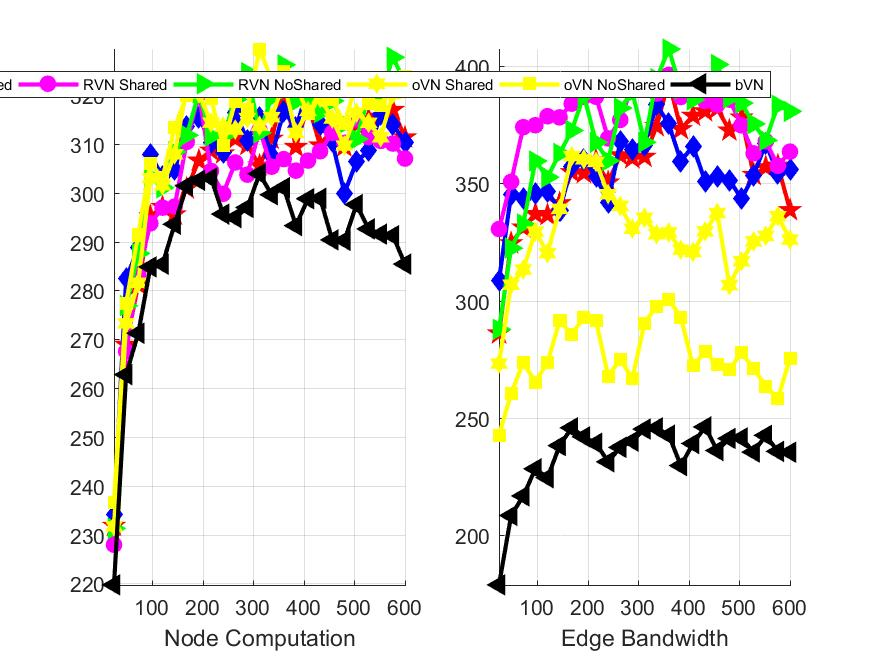
\includegraphics[width=3in]{Fig/CostCurrentSubstrateNetwork}\\
  \caption{Substrate Network Real-Time Cost}\label{fig:CostCurrentSubstrateNetwork}
\end{figure}

Substrate Network Increment Cost Fig.\ref{fig:CostAccumulateSubstrateNetwork}:
\begin{figure}[htbp]
  \centering
  % Requires \usepackage{graphicx}
  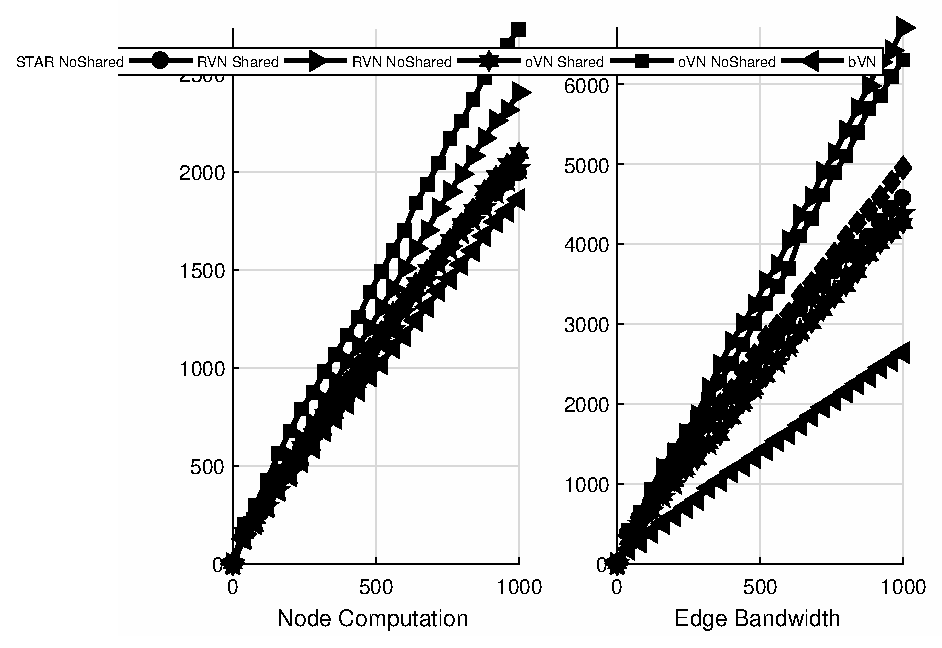
\includegraphics[width=3in]{Fig/CostAccumulateSubstrateNetwork}\\
  \caption{Substrate Network Increment Cost}\label{fig:CostAccumulateSubstrateNetwork}
\end{figure}

Substrate Network Average Real-Time  Cost Fig.\ref{fig:CostCurrentAverageSubstrateNetwork}:
\begin{figure}[htbp]
  \centering
  % Requires \usepackage{graphicx}
  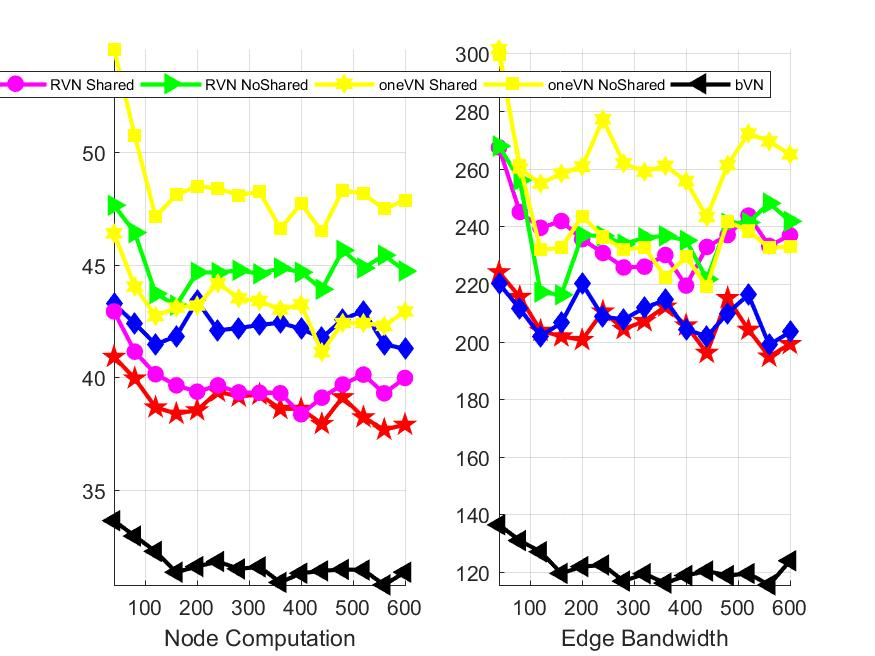
\includegraphics[width=3in]{Fig/CostCurrentAverageSubstrateNetwork}\\
  \caption{Substrate Network Average Real-Time Cost}\label{fig:CostCurrentAverageSubstrateNetwork}
\end{figure}

Substrate Network Increment Average Cost Fig.\ref{fig:CostAccumulateAverageSubstrateNetwork}:
\begin{figure}[htbp]
  \centering
  % Requires \usepackage{graphicx}
  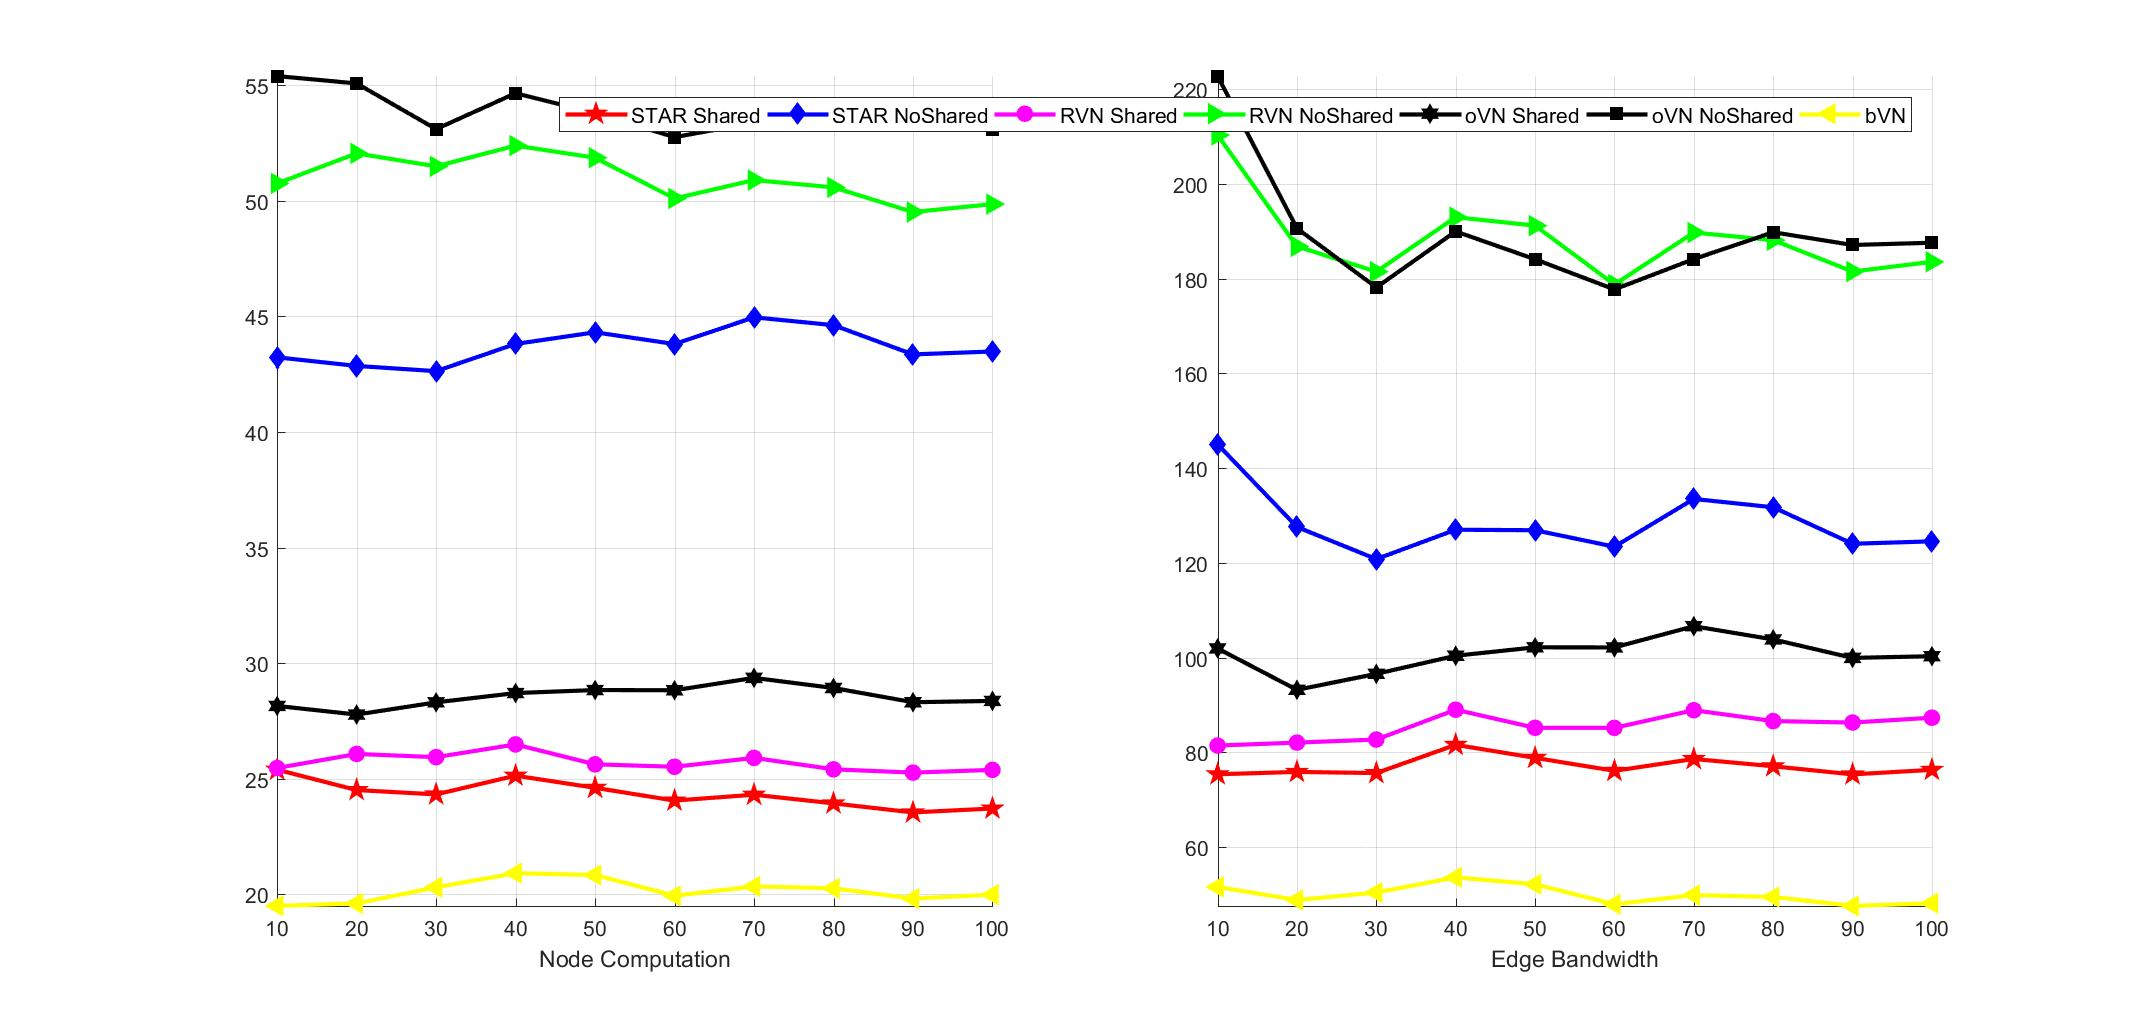
\includegraphics[width=3in]{Fig/CostAccumulateAverageSubstrateNetwork}\\
  \caption{Substrate Network Average Increment Cost }\label{fig:CostAccumulateAverageSubstrateNetwork}
\end{figure}



\subsubsection{Revenue}
Virtual Network Real-Time Revenue Fig.\ref{fig:RevenueCurrentVirtualNetwork}:
\begin{figure}[htbp]
  \centering
  % Requires \usepackage{graphicx}
  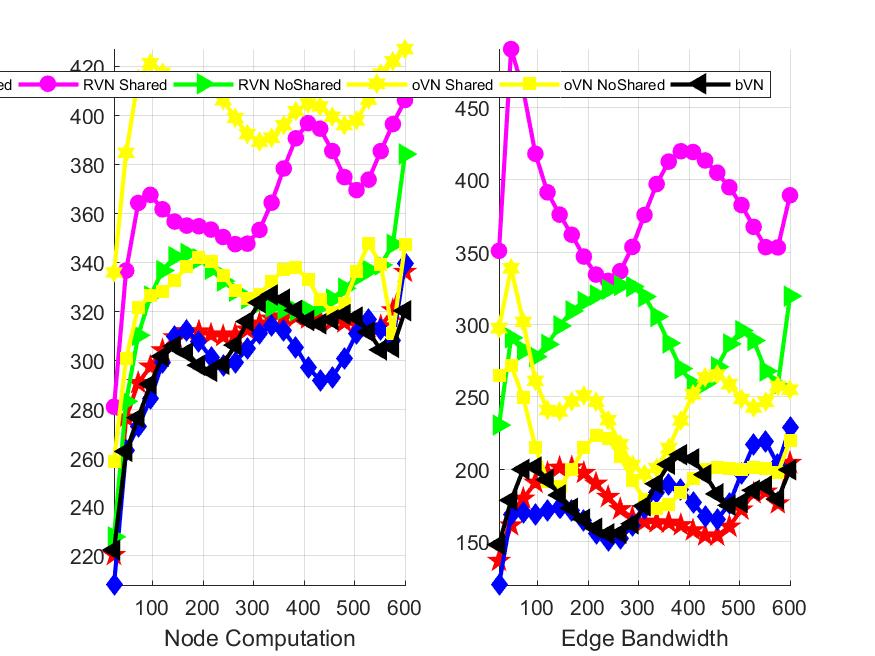
\includegraphics[width=3in]{Fig/RevenueCurrentVirtualNetwork}\\
  \caption{Virtual Network Real-Time Revenue }\label{fig:RevenueCurrentVirtualNetwork}
\end{figure}

Virtual Network Increment Revenue Fig.\ref{fig:RevenueAccumulateVirtualNetwork}:
\begin{figure}[htbp]
  \centering
  % Requires \usepackage{graphicx}
  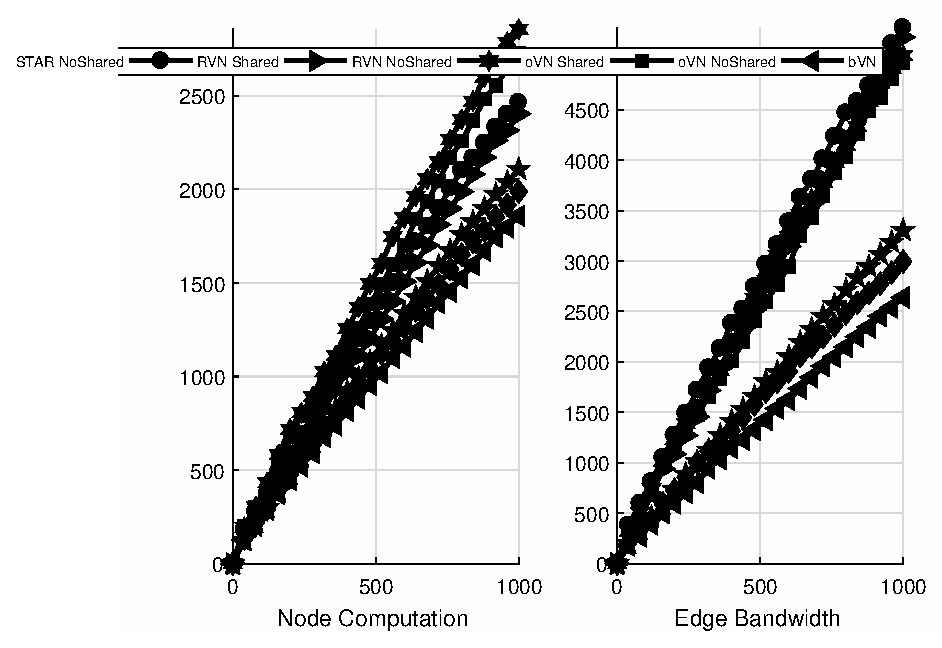
\includegraphics[width=3in]{Fig/RevenueAccumulateVirtualNetwork}\\
  \caption{Virtual Network Increment Revenue }\label{fig:RevenueAccumulateVirtualNetwork}
\end{figure}

Virtual Network Average Real-Time Revenue Fig.\ref{fig:RevenueAverageCurrentVirtualNetwork}:
\begin{figure}[htbp]
  \centering
  % Requires \usepackage{graphicx}
  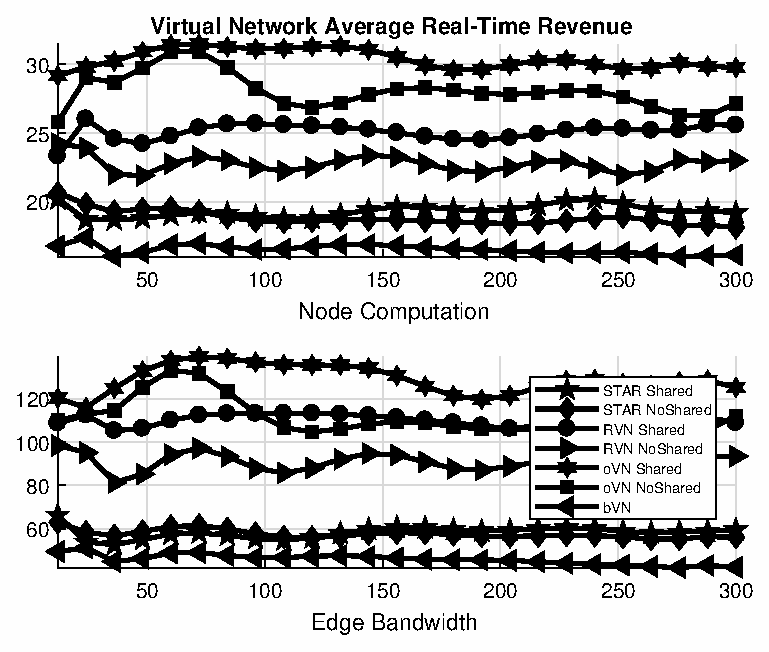
\includegraphics[width=3in]{Fig/RevenueAverageCurrentVirtualNetwork}\\
  \caption{Virtual Network Average Real-Time Revenue}\label{fig:RevenueAverageCurrentVirtualNetwork}
\end{figure}

Virtual Network Average Increment Revenue Fig.\ref{fig:RevenueAccumulateAverageVirtualNetwork}:
\begin{figure}[htbp]
  \centering
  % Requires \usepackage{graphicx}
  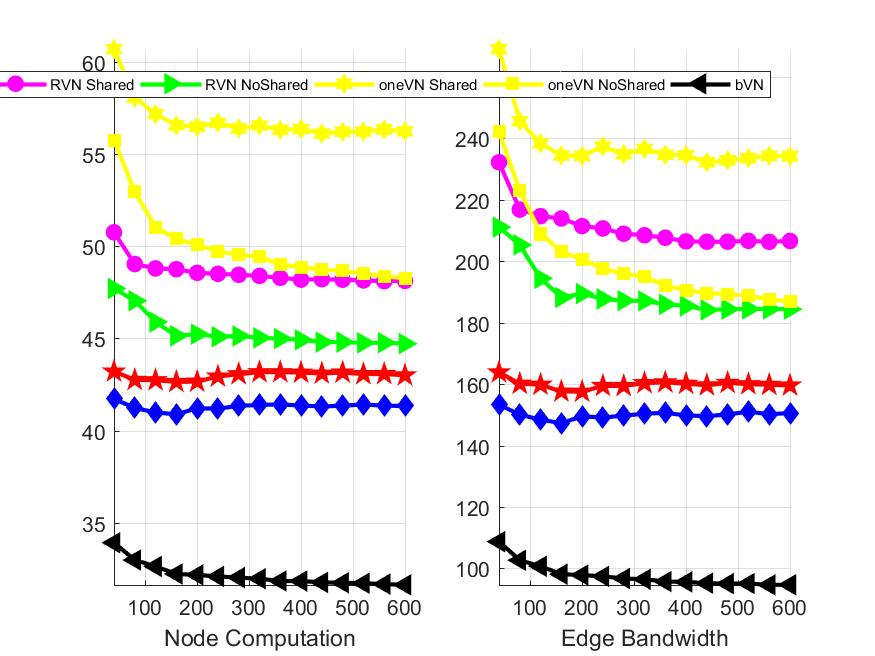
\includegraphics[width=3in]{Fig/RevenueAccumulateAverageVirtualNetwork}\\
  \caption{Virtual Network Average Increment Revenue}\label{fig:RevenueAccumulateAverageVirtualNetwork}
\end{figure}


\subsubsection{Cost/Revenue}
By dividing Cost by Revenue, varying Cost values are balanced. The higher the value, the more resources were needed to embed the SeVNs.

Cost/Revenue Fig.\ref{fig:CostRevenue}:
\begin{figure}[htbp]
  \centering
  % Requires \usepackage{graphicx}
  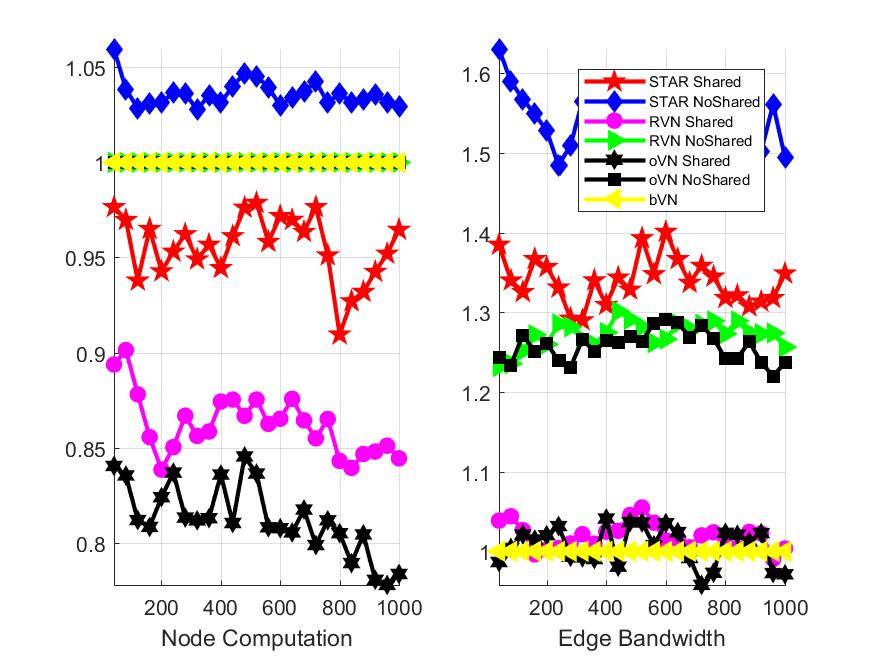
\includegraphics[width=3in]{Fig/CostRevenue}\\
  \caption{Cost/Revenue}\label{fig:CostRevenue}
\end{figure}

Increment Cost to Increment Revenue Fig.\ref{fig:CostRevenueAccumulate}:
\begin{figure}[htbp]
  \centering
  % Requires \usepackage{graphicx}
  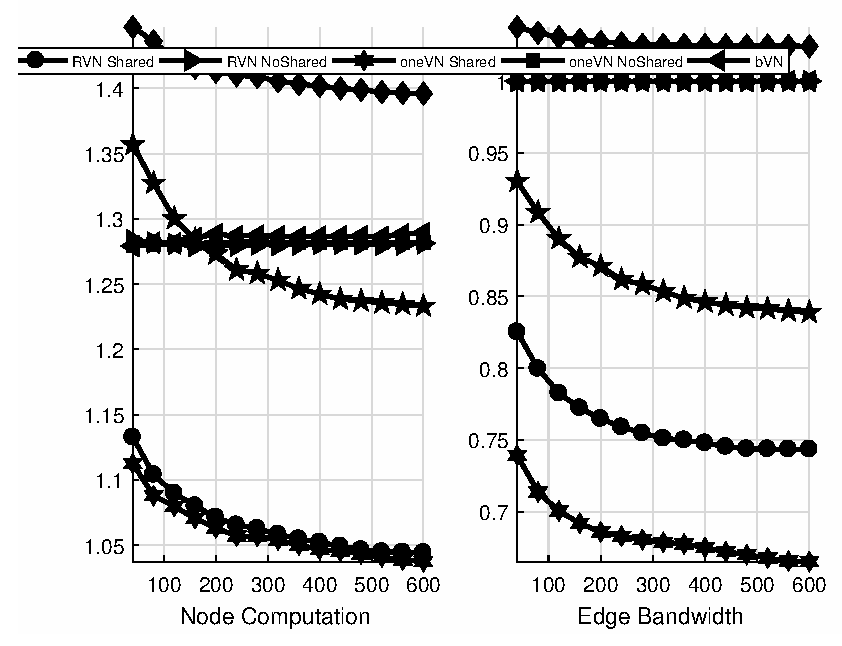
\includegraphics[width=3in]{Fig/CostRevenueAccumulate}\\
  \caption{Increment Cost/Increment Revenue}\label{fig:CostRevenueAccumulate}
\end{figure}



\subsection{Migration Frequency}
Typically, at least the virtual nodes hosted on the failing substrate nodes have to be moved. Other constraints, like maximum path length, might however trigger even more migrations. Since migrations are resource intensive, they should be kept to a minimum.
Fig.\ref{fig:MigrationFrequence}
\begin{figure}[htbp]
  \centering
  % Requires \usepackage{graphicx}
  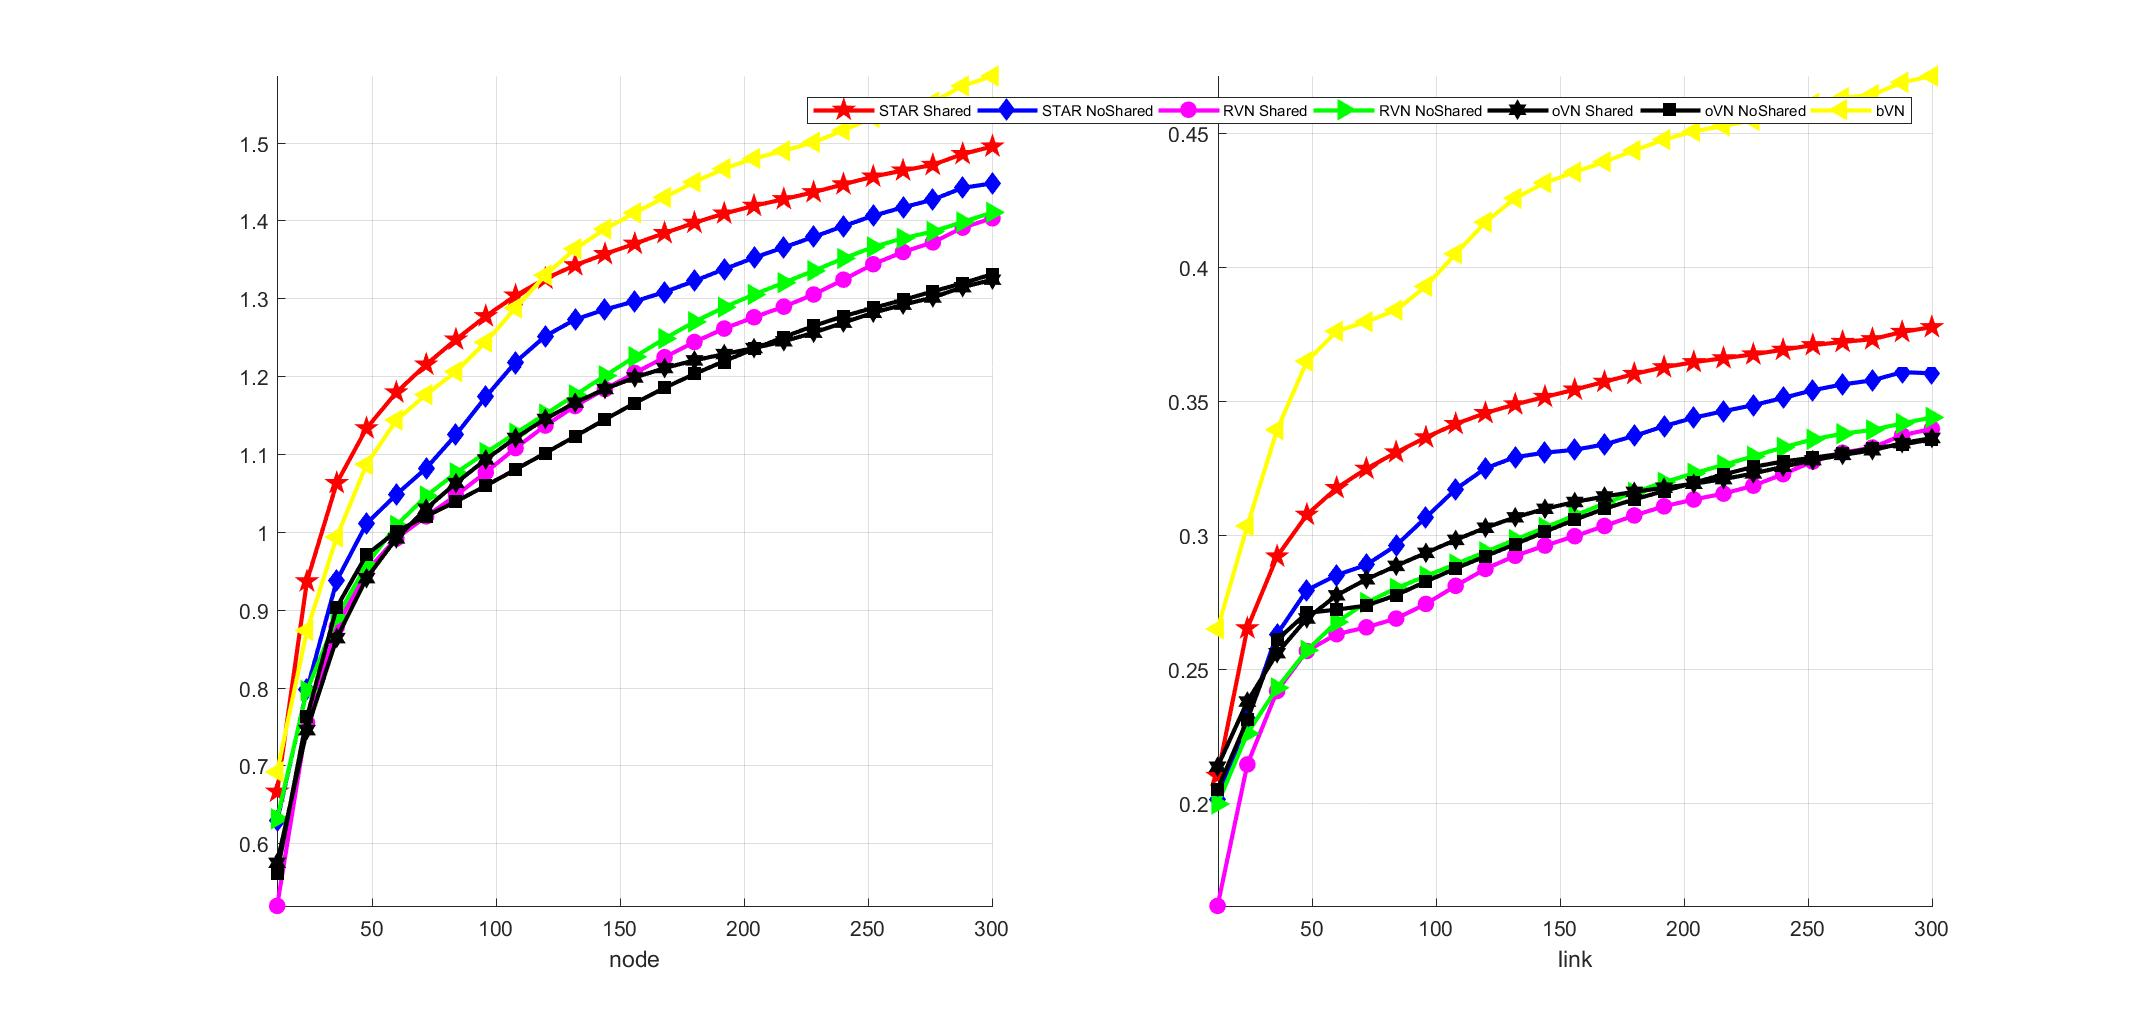
\includegraphics[width=3in]{Fig/MigrationFrequence}\\
  \caption{Migration Frequency Ratio}\label{fig:MigrationFrequence}
\end{figure}
%As mentioned above, FD-EVN algorithms achieve higher acceptance ratio and lower embedding cost at the cost of more node migration after facility node failure, which would cause service interruption and should be examined carefully, especially for the application with SLA constraints. We run our simulation in $\SubstrateNewtorkRunTimeInterval$ time unites, which corresponds to about $\SubStrateFacilityNodeFailDuration$ requests on average in each instance of simulation. The migration frequency
%after random facility node  failure is presented in Fig. 8 in terms of the number of VN nodes.


\subsection{Stress}
The stress level of a substrate entity reflects the number of virtual entities that are mapped onto it. The more virtual enti ties use the same substrate resource, the higher the impact regarding possible side effects. For example, mapping many virtual nodes onto a single substrate node keeps the CPU of the host operating system busy. A high substrate link stress might result in some additional packet delay because the resources of the substrate link and the host interfaces communicating through this link have to be shared
between virtual entities.
The stress of a SN element (node or link)is the number of virtual instances mapped on top of it.
Stress Fig.\ref{fig:Stress}:
\begin{figure}[htbp]
  \centering
  % Requires \usepackage{graphicx}
  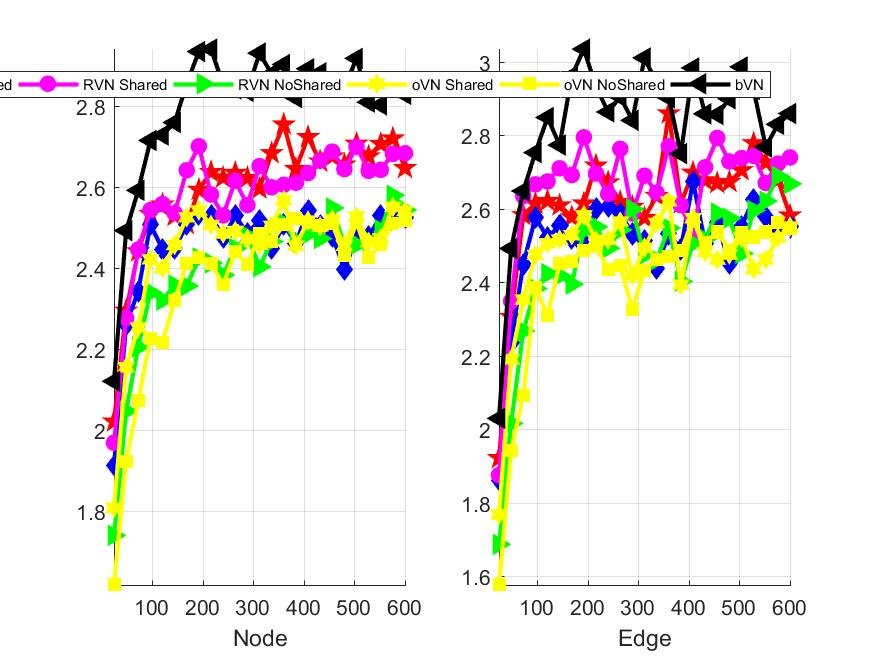
\includegraphics[width=3in]{Fig/Stress}\\
  \caption{Stress}\label{fig:Stress}
\end{figure}


\subsection{Utilization}
Utilization measures, in each SN entity (node or link), the sum of the spent substrate resources due to the mapping of virtual entities divided by the total amount of resources. This metric is a more precise measurement tool than
the stress level metric, because it also takes into account the magnitude of the resource usage instead of simply counting the number of virtual entities that use a resource. For example, to measure the utilization of a substrate node, the sum of mapped computing resources divided by the node computing capacity of the node could be used. The usage of a substrate link could be based on the sum of mapped bandwidth resources divided by the total link bandwidth capacity.

Utilization Fig.\ref{fig:Utilization}:
\begin{figure}[htbp]
  \centering
  % Requires \usepackage{graphicx}
  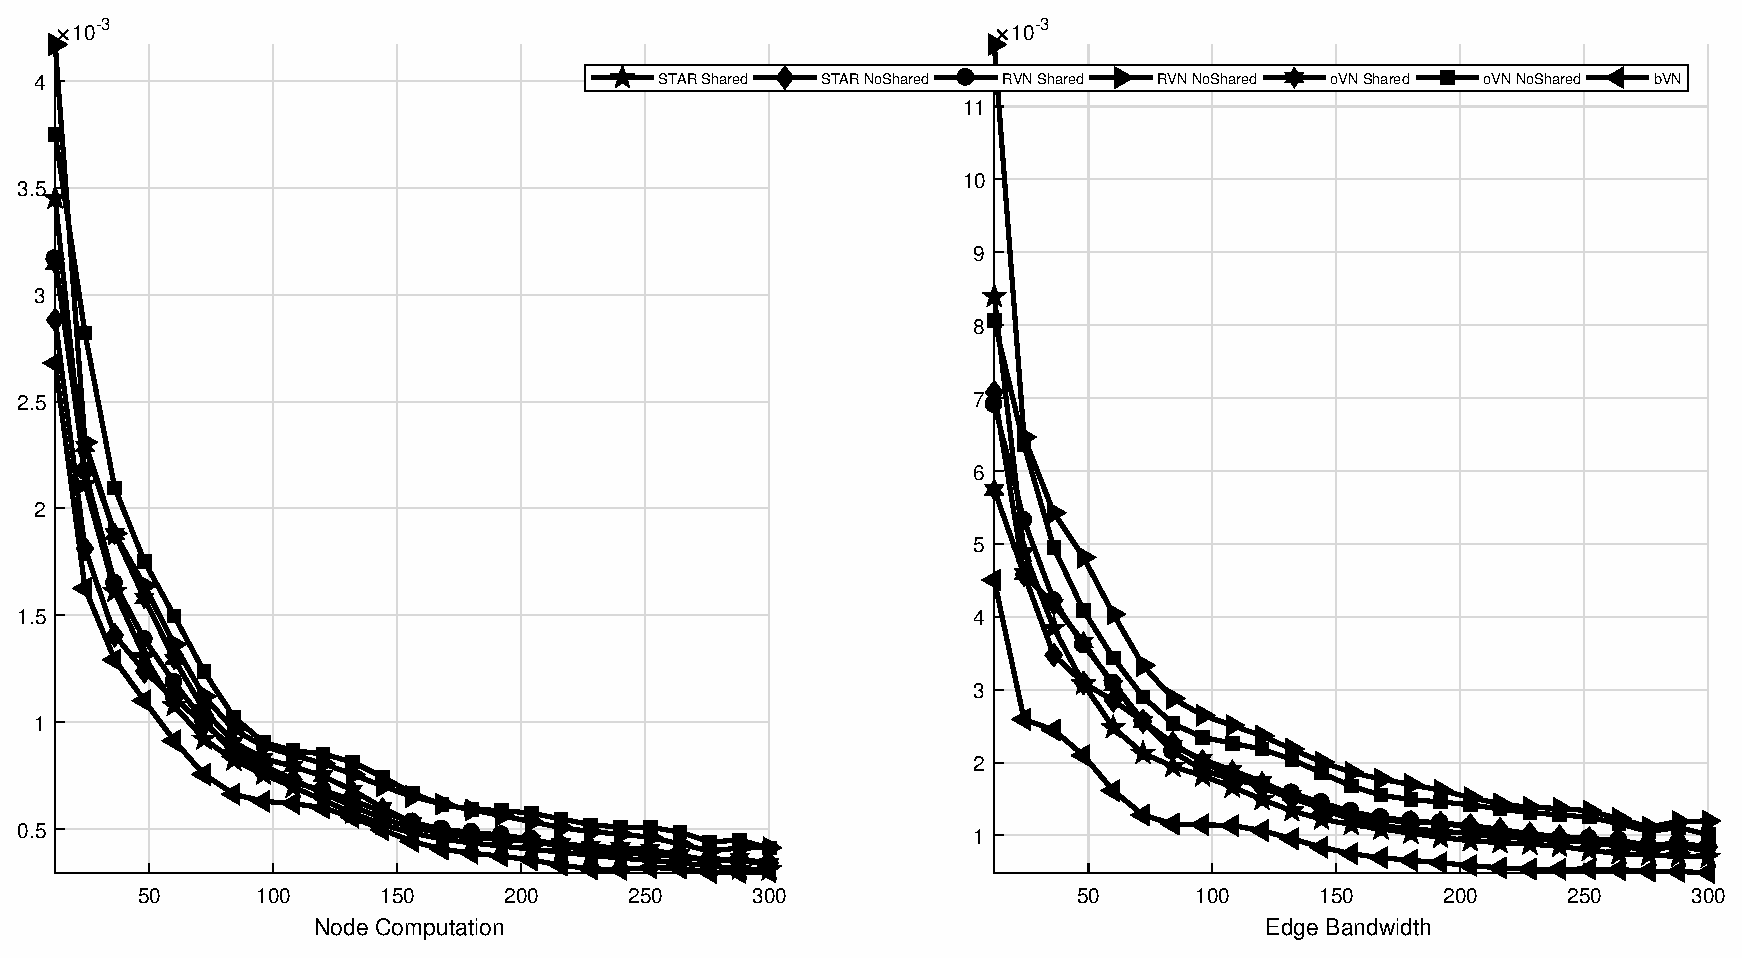
\includegraphics[width=3in]{Fig/Utilization}\\
  \caption{Utilization}\label{fig:Utilization}
\end{figure}


%\begin{figure*}
%  \centering
%  % Requires \usepackage{graphicx}
%
%
%
% \begin{equation*}
%\left[ {\begin{array}{*{20}{c}}
%&C_{P_{2.2}}&C_{P_{2.3}}&C_{P_3}&C_{P_4}&C_{B_{1.1}}&C_{B_{1.2}}&C_{B_{2.1}}&C_{B_{2.4}}&C_{B_{3.2}}&C_{B_{3.2}}\\
%{R_{V_1}}&\infty&\infty&\infty&\infty&\fbox{N+(2)+4+5+3}&\infty&${N+(2)+4+5+3}$&\infty&\infty&\infty\\
%R_{V_2}&\fbox{4}&\infty&\infty&\infty&\infty&${N+(3)+4+6}$&\infty&\infty&${N+(3)+4+6}$&\infty\\
%R_{V_3}&\infty&${M+(2)+5}$&\fbox{5}&\infty&\infty&\infty&\infty&\infty&\infty&${N+(5)+5+6}$\\
%R_{V_4}&\infty&\infty&\infty&\fbox{3}&\infty&\infty&\infty&${N+(6)+3}$&\infty&\infty\\
%\end{array}} \right]
%\end{equation*}
% \begin{equation*}
%\left[ {\begin{array}{*{20}{c}}
%&C_{P_{1}}&C_{P_3}&C_{P_4}&C_{B_{1.1}}&C_{B_{1.2}}&C_{B_{2.1}}&C_{B_{2.4}}&C_{B_{3.2}}&C_{B_{3.2}}\\
%{R_{V_1}}&4&\infty&\infty&${M+4}$&\infty&$N+(2)+4+5+3$&\infty&\infty&\infty\\
%R_{V_2}&\infty&\infty&\infty&\infty&${M+(1)+4+1} $&\infty&\infty&${N+(3)+4+6}$&\infty\\
%R_{V_3}&\infty&6&\infty&\infty&\infty&\infty&\infty&\infty&$N+(5)+5+6$\\
%R_{V_4}&\infty&\infty&0&\infty&\infty&\infty&$N+(6)+3$&\infty&\infty\\
%\end{array}} \right]
%\end{equation*}
%
% \begin{equation*}
%\left[ {\begin{array}{*{20}{c}}
%&C_{P_{1}}&C_{P_{2.2}}&C_{P_{2.3}}&C_{P_4}&C_{B_{1.1}}&C_{B_{1.2}}&C_{B_{2.1}}&C_{B_{2.4}}&C_{B_{3.2}}&C_{B_{3.3}}\\
%R_{V_1}&\fbox{5}&\infty&\infty&\infty&M+5&\infty&${N+(2)+4+5+3}$&\infty&\infty&\infty\\
%R_{V_2}&\infty&\mbox{6}&\infty&\infty&\infty&\fbox{M+6}&\infty&\infty&${N+(3)+4+6}$&\infty\\
%R_{V_3}&\infty&\infty&\fbox{M+(2)+1}&\infty&\infty&\infty&\infty&\infty&\infty&${N+(5)+5+6}$\\
%R_{V_4}&\infty&\infty&\infty&\fbox{0}&\infty&\infty&\infty&${N+(6)+3}$&\infty&\infty\\
%\end{array}} \right]
%\end{equation*}
%\end{figure*}





%\end{CJK*}

%\appendix
%This appendix will try to clarify themain differences between
%the considered heuristics. The network which will be used

\subsection{Conclusion}
In this paper, We propose an efficient algorithm $\MyAlgorithmMethodAbrreviation$ to efficiently solve allocating augmented resources (starting new physical node, link bandwidth or node computation) of the $\MyProblemAbrreviation$  problem in a substrate network for embedded virtual network with survivability guarantees request, which is guaranteed through redundant nodes and links. The resource allocation approach regards whether the redundant nodes are passive or reactive so long as ample resources are available when recovering from failures.

Since a physical infrastructure(substrate network) hosts multiple VNs, it is more resource efficient to share redundant nodes between VN. To reduce the allocated resource for survivability guarantees. We introduced a heuristic method to share these redundancies for both independent and cascading types of failures and do the best to minimum allocated resource based on Star-Constructer decomposition and dynamic programming.

Our algorithm take a novel allocate resource method for reducing new-booting hosts and minimizing resource with limited process time, in addition, Integer Program can not calculate out the optimal solution even the scale of problem is relatively small. The simulation results demonstrate that our algorithm have significant impact in conserving resources, achieving high acceptance rates ,high resource utilization and low number of active node.

\bibliographystyle{ieeetr}
\bibliography{BibNFT}

\end{document}
%\section{EeVSN Formulation}
After designing an EVN, in this section, we also formulate
its embedding problem as an MILP fitting for both FD-EVN
and FI-EVN embedding, since the difference between them in
embedding approach could be reconciled by a general resources
sharing constraint. More details would be elaborated in the following
part.

with respect to the node embedding, we
have the assumption that all the virtual nodes in EVN should be
mapped on physically isolated substrate nodes.

different node failure scenarios.
Thus, rather than solving the link embedding problem based
on the multi-commodity flow LP, we need consider the resource
sharing issues, which is computational intractable. As a result,
heuristic algorithms with acceptable computation complexity.


%\section{EeVSN Design Formulation}



